\documentclass[a4paper,12pt]{thesis}

\usepackage[utf8]{inputenc}

\usepackage{blindtext}

\usepackage{subfig}

\usepackage[onehalfspacing]{setspace}

\usepackage{adjustbox}
\usepackage[ngerman]{babel}
\usepackage[T1]{fontenc}
\usepackage{amsfonts}
\usepackage{amsmath}
\usepackage{mathtools} 
\usepackage{mathabx}
\usepackage{graphicx}
\usepackage[table]{xcolor}
\usepackage{longtable}
\usepackage{csvsimple}
%\usepackage{hyperref}

\usepackage{setspace}

\usepackage{color}
\usepackage{transparent}

\usepackage{tikz}
\usetikzlibrary{positioning}
\usetikzlibrary{arrows,calc}
%\usepackage{pgfplots} % LaTeX
\usepackage{colortbl}
%\usepackage{pgfplotstable}
\usepackage{booktabs, colortbl}

\usepackage{eurosym}


\usepackage{acronym}

\usepackage{listings}
\lstset{
	frame=single,
	language=R,
	keywordstyle=\color{blue},
	commentstyle=\color{green},
	numbers=left,
}

\usepackage[authoryear]{natbib}
%\bibliographystyle{apalike}
\usepackage[hidelinks]{hyperref}
\bibliographystyle{apalike}

\newcommand*{\captionsource}[2]{%
	\caption[{#1}]{%
		#1%
		\\\hspace{\linewidth}%
		\textbf{Quelle:} #2%
	}%
}

\tikzset{
%Define standard arrow tip
>=stealth',
%Define style for different line styles
help lines/.style={dashed, thick},
axis/.style={<->},
important line/.style={thick},
connection/.style={thick, dotted},
}


\begin{document}

%%% TITELSEITE %%%

\begin{center}								% Beginn einer center-Umgebung. Der Text innerhalb der center-Umgebung wird zentriert. Ansonsten wird Blocksatz verwendet
	\begin{LARGE}								% LARGE beschreibt eine Schriftgröße in Latex. Der Standard ist \normalsize. Eine übersicht der Schriftgrößen steht z.B. auf der Seite: https://www.latex-kurs.de/fragen/schriftgroesse.html 
		Räumliche Vorhersage des urbanen Radverkehrs mit Machine Learning					% Text, der nun zentriert und in größerer Schrift geschrieben wird 
	\end{LARGE}								% Die Verwendung der Schriftgröße LARGE wird beendet. Es gilt ab jetzt wieder die normale Schriftgröße.
	
	\vspace{\fill}								% Befehl, der den vertikalen Platz (vspace) "füllt" 
	
	\begin{large}								% Der folgende Text hat nun die Schriftgröße large 
		Maximilian Samuel Weinhold\\					% Durch ein \\ wird eine neue Zeile angefangen. 
		Economics, 7. Semester\\
		505314\\
		mweinhol@uni-muenster.de\\
		
		\vspace{\fill}
		
		Masterarbeit\\
		Wintersemester 2022\\
		Institut für Verkehrswissenschaft\\
		Prof. Dr. Gernot Sieg\\
	\end{large}
	
	\thispagestyle{empty}						% Definiert den Stil für diese Seite. empty bedeutet, dass keine Seitenzahl auf der Seite gedruckt wird. 
	
\end{center}								% Ab nun wird wieder Blocksatz verwendet

\newpage									% Seitenumbruch. Es beginnt eine neue Seite


%\chapter*{Tabellen und Abbildungen}\addchapmark{Tabellen und Abbildungen}
\onehalfspacing	
\thispagestyle{empty}
\setcounter{tocdepth}{1}
\tableofcontents

\begingroup
\let\clearpage\relax
\listoffigures
\listoftables
\endgroup

\section{Abkürzungsverzeichnis}

\begin{acronym}
	\acro{ZIV}{Zweirad-Industrie-Verband}
	\acro{OLS}{Ordinary Least Square}
	\acro{bzw.}{beziehungsweise}
	\acro{z.B.}{zum Beispiel}
	\acro{u.a.}{unter anderem}
\end{acronym}

%ReLU (Rectified-Linear-Unit)
%RMSE (Root Mean Squared Error)

\chapter{Einleitung}

Vielerorts erlebt der Individualverkehr eine Renaissance des Fahrradfahrens. So ist laut \cite{Eisenberger2015} und dem Verband der Zweirad Industrie \cite{ZIV2022} der Bestand an Fahrrädern in Deutschland von 72 Mio. in 2015 auf 81 Mio. in 2021 angestiegen. Der anhaltende Boom hat viele Gründe. Im Vergleich zum Auto ist die bewegungsintensivere Fortbewegung auf dem Fahrrad gesünder, schont die Umwelt und das Portemonnaie.\\
Viele Kommunen entscheiden sich u.a. aus diesen Gründen dafür, ihre Stadt fahrradfreundlicher zu gestalten. So unterstützt das Bundesministerium für Verkehr und digitale Infrastruktur \cite{VerkehrunddigitaleInfrastruktur2020} die Länder und Gemeinden beim Ausbau von Radwegen durch eine direkte Hilfe in Höhe von 660 Mio. Euro bis 2023.\\
Dies, sowie der genaue lokale Bedarf und die Auslastung von Fahrradwegen, muss bei der Planung der Infrastruktur beachtet werden. Motiviert ist diese Arbeit mit dem Wunsch, Antworten auf mögliche Fragen der Infrastrukturplanung bieten zu können. Die Forschungsfrage, die sich daraus ableitet, lautet: Ist es möglich, ein räumliches Modell zu entwickeln, das für ein vollständiges Straßennetz oder für ausgewählte flexible Knotenpunkte zu bestimmten Zeiten Vorhersagen zum Fahrradverkehr machen kann und lassen diese auch zusätzlich die gefährlichsten Stellen für Fahrradunfälle erkennen? Ziel dabei ist es, eine Anleitung zu Erstellung solcher Modelle zu geben.\\
Dazu beginnt diese Masterarbeit mit einem Einblick in die bestehende Literatur, welcher kategorisiert ist nach Daten und Faktoren. Häufig verwendete Methoden werden im Nachgang näher beschrieben. Das erworbene Wissen dient dazu, ein Modell zu entwickeln, dass im Rahmen dieser Abschlussarbeit auch evaluiert wird. Im Anschluss wird analysiert, wie sehr das Radverkehrsaufkommen mit Radverkehrsunfällen räumlich korreliert.

\chapter{Literaturüberblick}

Die Auslastung von Fahrradwegen, bzw. das Aufkommen von Fahrrädern, beruht im Wesentlichen auf der individuellen Entscheidung eines jeden Fahrers, das Fahrrad einer anderen Transportalternative vorzuziehen. Versteht man die Faktoren, aus denen sich diese Entscheidung zusammensetzt, dann kann man leichter eine solche Entscheidung vorhersagen. Mit einer Zusammenfassung der bisherigen Literatur wollen \cite{Heinen2010} diese Faktoren aufzeigen, wobei sie sich hier nur auf Pendler beschränken. Zum einem ist einer dieser Faktoren die bauliche Substanz, die nicht nur die Radwege sondern auch Abstellmöglichkeiten und Ampeln wie auch Verkehrsschilder beinhaltet, zum anderem spielt auch das Wetter eine große Rolle. Einen negativen Effekt hat die Rate der Autobesitzer und natürlich auch die Verfügbarkeit anderer Transportmöglichkeiten.\\

\section{Erforschung des Radverkehrs}

Seitdem erschienen zahlreiche weitere empirische Studien, die das Bild über den Radverkehr konkretisieren. Diese verschiedenen Studien lassen sich nach Datenquellen kategorisieren. Die meisten nutzen drei verschiedene Datengrundlagen zur Modellierung des Fahrradverkehr in Verbindung zu Daten mit anderen Faktoren. Die drei Datenquellen zum Fahrradverkehr stammen von Fahrradzählstation, einer Induktionsschleife die darüber fahrende Räder verifiziert, Daten von Bike-Sharing-Diensten und Daten verschiedener GPS und Handy Applikationen.\\

\subsection{Forschung mit Zählstationen}

In Deutschland findet sich eine weite Verbreitung von Fahrradzählstationen in verschiedenen Städten, deren Daten oft öffentlich einsehbar sind. Deswegen wäre eine Verwendung dieser Datengrundlage überaus naheliegend. Studien, die ähnliche Daten verwenden, stammen z.B. von \cite{Holmgren2017}, \cite{Broucke2019}, \cite{Wessel2020} und \cite{Goldmann2021}. Die Arbeit von \cite{Wessel2020} wird in einem späteren Abschnitt behandelt, in dem es mehr um den kausalen Zusammenhang von Fahrradverkehr und Wetter geht. \cite{Holmgren2017} verwenden tägliche Daten von 2006 bis 2014 aus Malmö und verbinden diese ebenfalls wie später bei \cite{Wessel2020} mit Wetterdaten, Feiertagen und Schulferien. Als Methode zur Auswertung dieser Daten und zur Schätzung des Fahrradaufkommens verwenden sie Random-Forest-Regressionssysteme, Support-Vector-Regression, eine lineare Regression und ein Multy-Layer-Perceptron, also ein neuronales Netz. Im Vergleich dieser Methoden erzielten sie die treffsichersten Resultate mit einem Regressionsbaum und der Support-Vector-Regression, welche auf quadratische und kubische Kernels zurückgreift. Mithilfe des Support-Vector-Regressionssystems kommen sie auf ein Bestimmtheitsmaß R$^2$ von 86,9 \%.\\
Um diese Methoden zu vergleichen nutzen \cite{Holmgren2017} die Cross-Validation. Ähnlich gehen \cite{Broucke2019} vor und verwenden dabei Daten von 12 Zählstationen aus Brüssel. Sie verbinden diese Daten mit temporalen, geographischen und meteorologischen Daten. Ebenfalls verwenden sie eine Support Vector Regression, die auf einer Radial-Basis-Funktion aufbaut, um eines ihrer vier Modelle zu berechnen. Für die anderen drei verwenden sie Random-Forest-Regression, welche auf Zufallsbäume aufbaut, ein Gradient-Boosting-Modell und ein voll verknüpftes neuronales Netzwerk. Letzteres beinhaltet 2 Schichten mit einmal 28 und einmal 14 Knoten, die die ReLU (Rectified-Linear-Unit) Funktion als Aktivierung verwenden. Von allen Modellen mit Wetterdaten erzielt das neuronale Netzwerk hier den niedrigsten RMSE (Root Mean Squared Error) und schneidet somit am besten ab.

\subsection{Forschung mit Bike-Sharing-Diensten}

Die überragende Mehrheit an Studien zur Schätzung und Vorhersage des Fahrradverkehrs verwendet Daten von Bike-Sharing-Diensten, dazu zählen \cite{Kaltenbrunner2010}, \cite{Xu2013}, \cite{Li2015}, \cite{Mitchell2018PredictingBT}, \cite{Colace2020}, \cite{Gao2022} und \cite{Li2022}. Dies ist natürlich immer noch nur eine Auswahl an Studien. Die Literatur zu Bike Sharing Systemen ist sehr ausführlich. Eine weitere Übersicht hierzu findet sich bei \cite{Mitchell2018PredictingBT}.\\
\cite{Kaltenbrunner2010} nutzen z.B. Daten von 400 öffentlichen Rad Ausleihstationen in Barcelona. Ihre Studie hegt die Absicht, die Effizienz des bestehenden Verleihsystems in Barcelona, das zu dem Zeitpunkt um die 180000 Abonnenten hatte, zu verbessern. Hier geht es also eher darum, vorherzusagen, wie viele Fahrräder sich in welcher Ausleihstation zu welchem Zeitpunkt befinden, um den Nutzern detaillierte Informationen zu geben.\\
Eine ähnliche Motivation haben \cite{Xu2013}. Diese verwenden Daten ihren Aussagen zufolge des größten öffentlichen Bike-Sharing-Systems der Welt in Hangzhou in China. Ihr Datensatz beinhaltet die aufgezeichnete Auslastung der Stationen einiger Tage und Wochen zuvor, sowie Daten zum aktuellen und vergangenem Wetter und Informationen über Feiertage. Diesen Datensatz normalisieren und clustern sie mit der k-Means Cluster Methode. Darauf wenden sie Support-Vector-Machines an, um die Gewichte der beschriebenen Estimatoren zu finden. Dieses hybride Modell hat nur noch eine Fehlerrate von 3,57 \% vergleicht man dessen Vorhersagen, mit den tatsächlich eingetretenen Auslastungen.\\
\cite{Li2015} stellen hier ein Paper zur Verfügung das ähnlich funktioniert. Auch sie wollen eine Ausbalancierung der Fahrradbestände an allen Stationen in New York und Washington DC erleichtern. Und genau wie \cite{Xu2013} unterteilen sie die Stationen in Cluster. Für diese Cluster wollen sie Vorhersagen machen, was zu robusteren Ergebnissen führt, als wenn man für jede einzelne Station Vorhersagen bildet. Zusätzlich verwenden \cite{Li2015} Wetter Beobachtungen in ihrem Datensatz. Darauf wird ein Gradient-Boosting-Regression-Tree angewendet. Gradient-Boosting besteht aus kurzläufigen zufälligen Entscheidungsbäumen, die der Reihe nach auf den Fehlerterm des vorherigen Entscheidungsbaumes beruhen und diesen versuchen zu verbessern.\\
Auf Cluster Level Bike-Sharing geht auch \cite{Mitchell2018PredictingBT} ein. Er evaluiert verschiedene Machine-Learning-Methoden miteinander: Random Forests, Fast-Feed-Forward-Neural-Networks, Deep-Residual-Networks und Recurrent-Neural-Networks.  Dabei schlagen sich die Feed-Forward-Neural-Networks am besten.\\
Einen besonderen Ansatz verfolgen \cite{Colace2020}, die Aufnahmen von Überwachungskameras in ihrer Analyse mit aufnehmen.\\
Eine besonders aktuelle Analyse stammte von \cite{Gao2022}. \cite{Gao2022} sind hierbei die Ersten von den bisher genannten, die mehr Informationen als nur Wetterberichte in ihrer Analyse aufnehmen. Aufbauend auf Daten zu 2098 Fahrradstationen aus Seoul nehmen sie in ihr Modell z.B. Feinstaubbelastungen mit auf, was \cite{Hong2022} und \cite{ZHAO2018826} als relevanten Faktor gezeigt haben. Daneben inkludieren sie auch Verkehrsdaten, Corona Fälle und sozioökonomische Daten, Verkehrsunfälle und Saisonalität. Darauf wenden sie lineare Regressionen, k-Nearest-Neighbour (knn), Random Forests und Support-Vector-Machines an. All diese Methoden wurden in der Programmiersprache R angewendet. Diese Modelle vergleichen sie mit einem Validation-Set-Schnitt von 75 \% für das Trainings Set und 25 \% für das Test Set. Damit betreiben \cite{Gao2022} eine Feature Selection, die auf den Boruta Algorithmus zurückgreift. Das Ziel von Feature Selektion hier ist, am Ende ein Modell zu haben, dass nur auf statistisch relevante Variablen zurückgreift. Dazu erstellt der Boruta Algorithmus nach \cite{Kursa2010} verschiedene unabhängige Bagging Samples, zieht daraus Classification-Trees und beurteilt die Features nach Verlust an Akkurarität. Die relevantesten Variablen waren das Wetter und die Anzahl der Corona Fälle. Mit einer 10-fold Cross Validation fanden sie heraus, dass sich die Support-Vector-Machines und die Random Forests am besten geschlagen haben. So lässt sich mit Random Forests ein Test R$^2$-Wert von 93 \% erreichen und mit Support-Vector-Machines ein Test R$^2$-Wert von 90 \%, was beides sehr gute Werte sind. Dabei spielten auch die sozioökonimische Daten eine Rolle, die im Gesamten zwar wenig Relevanz hatten, aber Unterschiede zwischen den Docking Stationen erklären konnten.\\ 
\cite{Li2022} möchten nicht nur den Bestand von Rädern an fixen Fahrradausleihstationen vorhersagen, sondern die generelle Nutzung und das Verkehrsvolumen von Leihrädern in einem Gebiet berechnen. Dieses Ziel geht schon eher in die Richtung der Fragesetllung dieser Masterarbeit, beschränkt sich jedoch auf Leihräder und nicht auf den gesamten Radverkehr. Dazu verwenden sie Daten von festen Fahrradstationen in Chicago und New York und Daten von Ausleihsystemen mit frei stehenden Fahrrädern die GPS Daten speichern in Singapore und New Taipei City. Jede Stadt zerteilen sie in ein Raster und wenden darauf Convolutional-Neural-Networks an, die auch oft für die Bilderkennung verwendet werden. Das Ergebnis dessen ist in der Abbildung \ref{LiBild} zu sehen.\\
\begin{figure}[!ht]
	\centering
	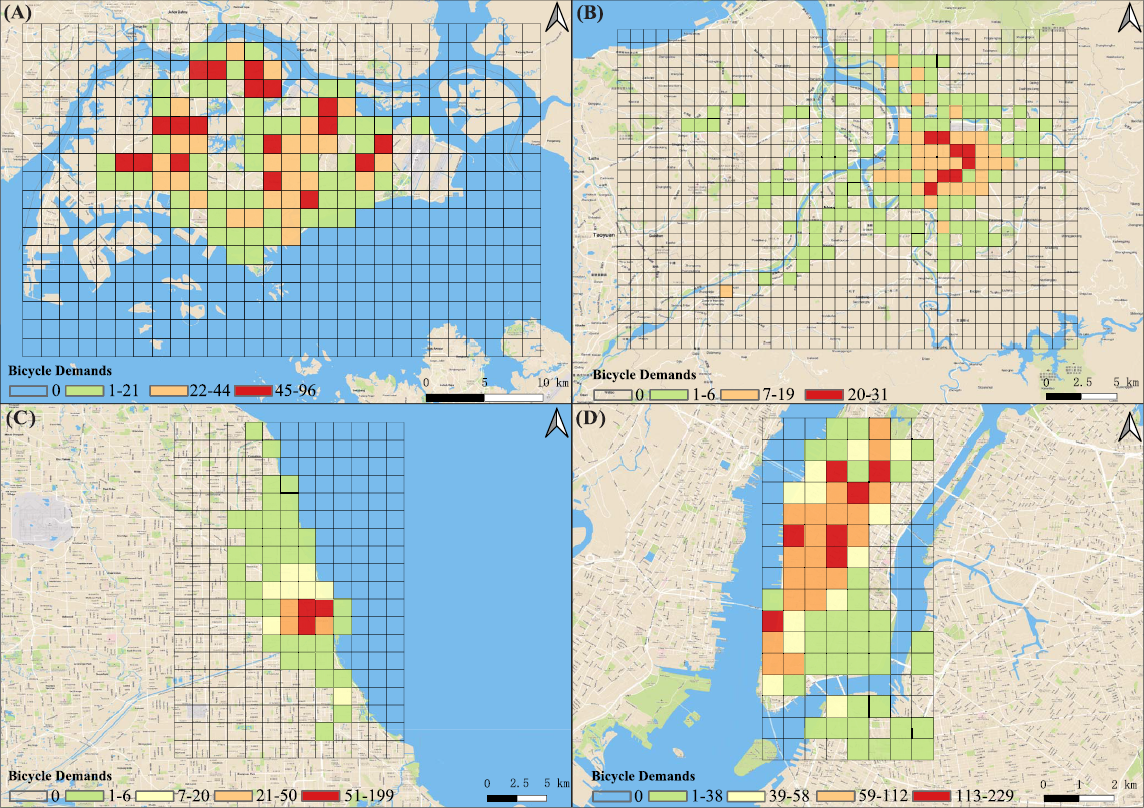
\includegraphics[width=\textwidth]{Plots/Li2022.png}
	\captionsource{Anzahl der Leihräder (A) Singapore zwischen 8-9 Uhr am 25. Juni 2017; (B) New Taipei City zwischen 18-19 Uhr am 1. August 2018; (C) Chicago zwischen 16-18 Uhr am 26. August 2019; (D) New York zwischen 17-18 Uhr am 9. Juni 2014.}{
		\cite{Li2022}
	}
	\label{LiBild}
\end{figure}
Eine Besonderheit dieser Arbeiten, die alle auf Daten von Bike-Sharing-Diensten beruhen, ist, dass sie mehr Datenpunkte in einer Stadt zur Verfügung haben als die Studien, die nur Daten von Zählstationen verwenden, da ein Netz von Leihstation eine höhere Dichte haben muss. So können \cite{Gao2022} z.B. 2098 Stationen in einer Stadt beobachten, während \cite{Broucke2019} z.B. nur 12 Zählstationen in einer Stadt zur Verfügung haben. Deshalb ergibt das Clustering von Bike-Sharing-Daten Sinn, wie es z.B. auch \cite{Xu2013} und \cite{Li2015} vornehmen.\\
Modelle die auf Zählstationen beruhen, können den gesamten Radverkehr an bestimmten Punkten messen und schätzen. Die hier kennen gelernten Modelle, die auf Bike-Sharing-Daten zurückgreifen, können das nicht, sondern ermitteln nur das Verkehrsvolumen, das von diesen Mieträdern kommt. Dafür können diese Modelle aber immer für den vollständige Verkehr dieser Mieträder schätzen. Interessant wäre die Frage, wie Mietradverkehr und Verkehr von Rädern in Privatbesitz miteinander korrelieren. Wer mit dem Fahrrad regulär pendelt, für den ist der Besitz eines Fahrrads langfristig kostengünstiger. So kann es sein, dass Spitzen in beiden Varianten von einander abweichen, weil Mieträder möglicherweise eher touristischen statt utilitaristischen Zwecken dienen. Mietraddaten allein sind also kein ausreichendes Mittel, um den gesamten Fahrrad Verkehr zu modellieren und sind gleichzeitig auch weniger zugänglich als Daten öffentlicher Zählstationen. Möglicherweise gäben aber Handy Daten mehr Aufschluss.

\subsection{Forschung mit GPS- und Handy Daten}\label{chpt:gps}


Schon im vorangegangenen Abschnitt zu den Daten von Bike-Sharing-Systemen haben \cite{Li2022} GPS-Daten von Leihfahrrädern für ihre Analyse genutzt. Doch das ist nicht die einzige Möglichkeit, um an GPS-Daten zu kommen. Ein weiterer Weg sind Handy Applikationen, die beständig GPS-Koordinaten aufzeichnen und damit Bewegungsprofile erstellen. \cite{Romanillos2016} stellen solche Studien vor, die auf GPS-Daten von Fitness und Leisure Applikationen zurückgreifen.\\ 
Eine der ersten Arbeiten wurde von \cite{Harvey2007} mit der Absicht erstellt, durch ihr Modell eine Priorisierung von Fahrradinfrastruktur zu ermöglichen. Dazu verwendeten sie noch GPS-Logging-Ausrüstung bei 51 Teilnehmern in einem Zeitraum von 3 Wochen in South Minneapolis, um favorisierte Radstrecken aufzuzeichnen. Neben der niedrigen Stichprobenmenge war diese Studie noch mit dem Problem des GPS-Cleanings konfrontiert, das zu Positionsabweichungen führen kann. Diese Probleme wurden von Folgestudien wie von \cite{Menghini2010} erstmals behoben, die in Zürich Daten von 2400 Teilnehmern hatten und mit einem verbessertem Detection Algorithmus auch Probleme des GPS-Post-Processing behoben haben.\\ 
Das Prinzip der GPS-Aufzeichnung entwickelte sich weiter und \cite{Reddy2010} verwendeten erstmals Handys als GPS-Logging-Geräte. Dazu verwenden sie Daten der App Biketastic. Das Problem bei Bike-Logging-Apps ist, dass hier eher Fahrrad Routen aufgezeichnet werden, die der Erholung dienen und nicht unbedingt dem alltäglichen utilitaristischen Stadtverkehr, da es sich oftmals um Apps handelt, die der sportlichen Aktivität dienen. Die Nutzung dieser Daten gibt also nicht Aufschluss über den gesamten Fahrradverkehr. Bei der hier genutzten Applikation Biketastic ist das jedoch anders, denn Biketastic wird speziell von Pendlern genutzt, um nicht nur GPS Daten aufzuzeichnen, sondern auch Fotos und Audioaufnahmen der Handys, um Straßen mit signifikant hohen Lärm ausfindig zu machen und so lauten Straßenverkehr in das Modell aufzunehmen. Bei der Evaluation stellte man schnell fest, dass Nutzer der App dazu tendierten, diese nur für lange Strecken zu nutzen, und sich nicht die Mühe machen, die App auf dem Handy zu betätigen, wenn man eine Strecke von unter einer Meile zurück legen wollte.\\
Eine weitere Studie stammte von \cite{Broach2012}, aber auch hier ist die Anzahl der Studienteilnehmer mit knapp über 164 gering. Weitere Studien in dem Bereich stammen von \cite{Musakwa2016}, \cite{Pritchard2018}, \cite{Lee2020} und \cite{Alattar2021}. Eine der aktuelleren Studien ist von \cite{Alattar2021}. Sie verwenden Daten, die durch die Fitness App Strava in Glasgow 2017 bis 2018 gewonnen wurden, um den Einfluss des Straßenlayouts auf die Routenwahl der Fahrer zu untersuchen. Dabei bauen sie auf ein räumliches Modell, das an bestimmten Straßenknotenpunkten stündliche durchgehende Fahrradfahrten nach Straße, Abfahrtsort und Zielort betrachtet. Um zu testen, wie gut die Strava Daten den tatsächlichen Radverkehr abbilden, wurde mit insgesamt 36 temporären Zählstation das Radverkehrsvolumen über zwei Tage stichprobenartig verglichen. Neben den Daten von Strava nutzten die Autoren das Python Paket OSMnx, dass direkten Zugang zu Open-Street-Map bietet. Open-Street-Map bietet umfassende Information über Glasgows Straßennetz und so können die Knotenpunkte mit dem Straßennetz verglichen werden. Das daraus resultierende Ergebnis ist in Abbildung \ref{Alattar_2021} zu sehen.
\begin{figure}[!ht]
	\centering
	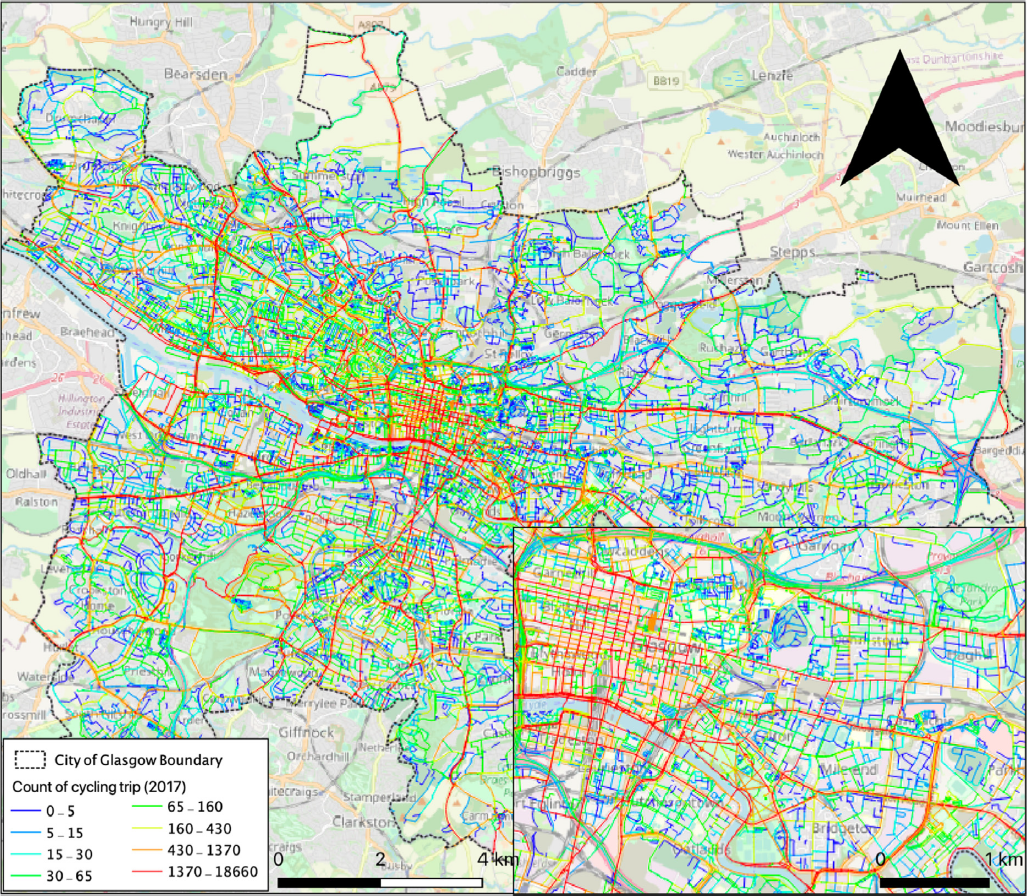
\includegraphics[width=\textwidth]{Plots/Alattar2021.png}
	\captionsource{Fahrradaufkommen für Glasgow 2017}{
		\cite{Alattar2021}
	}
	\label{Alattar_2021}
\end{figure}
Auf diese Daten kann nun eine Regression angewendet werden, deren erklärende Variablen logarithmerte Indikatoren der Zentralität innerhalb des Knotennetzwerkes sind, die die Anzahl der Fahrradtrips erklären sollen. Bei diesem Regressionsmodell kommt ein Erklärungswert R$^2$ von 42 \% zustande, was im Vergleich zu vorherigen Werten gering ist. Ein interessanter Forschungspunkt den \cite{Alattar2021} hätten hier noch verfolgen können, wäre wie sich die Vorhersagekraft ändert, wenn man Wetter, Feier und Ferientage in das Modell mit aufnimmt.\\
Die Studie von \cite{Alattar2021} geht mit der Räumlichkeit ihres Modells schon sehr in die Richtung der Forschungsfrage dieser Masterarbeit. Die Nutzung von Daten aus Open-Street-Map kann eine wesentliche Datenquelle sein. Das Ergebnis des Erklärungswertes von 42 \% im Modell von \cite{Alattar2021} sollte mindestens auch erzielt werden.\\
Im Überblick zeigen sich häufige Schwächen von Studien, die Handy Applikationsdaten nutzen wie den Strava-Datensatz. Zunächst unterliegen solche Apps häufig einer Selbstauswahl der Probanden. So sind z.B. in dem Datensatz von \cite{Alattar2021} Frauen unterrepräsentiert. Häufig dienen diese Apps der sportlichen Betätigung und nicht der Anfahrt zum Arbeitsplatz. Zudem sind ihre Daten schwer zugänglich.


\section{Faktoren des Radverkehrs}

Die Daten, die bisher am zugänglichsten waren, sind die Daten von Leihstationen. Mit ihnen lässt sich der Fahrradverkehr gut messen. Doch zielt die Forschungsfrage nicht darauf ab, den Radverkehr allein zu messen, sondern ihn vorherzusagen. Dazu benötigt es Daten, die im Zusammenhang mit dem Radverkehr stehen und einen wesentlichen Faktor bilden. Solche Faktoren können als Prädikator genutzt werden. Die Prädikatoren eines Modells spielen eine große Rolle, denn mit der Auswahl der richtigen Prädikatoren steht und fällt die Validität des Modells. Deswegen klärt ein gesonderter Literaturüberblick die Tragweite einzelner Variablen, die möglicherweise das Aufkommen an urbanen Fahrradverkehr erklären können. Wichtiges Attribut eines Prädikators ist zudem die Datenverfügbarkeit. 

\subsection{Faktor Wetter}

Der vorausgehende Abschnitt, der einen Blick auf die bestehende Literatur nahm, erwähnte oftmals Wetterdaten, die in verschiedenen Modellen genutzt worden, so z.B. bei \cite{Holmgren2017}, \cite{Broucke2019}, \cite{Li2015}. Literatur, die sich speziell mit diesem Zusammenhang beschäftigt, findet sich bei \cite{Wessel2020}. Dabei hat er sich z.B. im Gegensatz zu \cite{Nankervis1999}, der sich auch mit dem Zusammenhang von Wetter und Fahrrad Aufkommen beschäftigt, gezielt mit dem Zusammenhang von Wettervorhersagen beschäftigt. Auch \cite{Meng2016} untersucht diesen Zusammenhang.\\
Jedoch während \cite{Meng2016} Daten einer Umfrage von 553 Fahrradfahrern in Singapore verwendet, stützt sich \cite{Wessel2020} auf umfangreichere Daten von 188 Fahrradzählstationen in 37 deutschen Städten, die stündlich zählen. Daten zum aktuellen Wetter stammen vom Deutschen Wetterdienst. Daten über Wettervorhersagen stammen aus der ARD Mediathek, der abendlichen Tagesschau um acht Uhr. Die Aufzeichnungen der Wettervorhersagen worden dabei manuell ausgewertet, wobei der deutsche Raum in sechs Hemisphäre Nordwest, Nordost, mittlerer Westen und mittlerer Osten so wie Südwest und Südost unterteilt wurden und die Städte in die korrespondierende Hemisphäre eingeteilt worden sind nach folgenden Wetter Klassifikationen: klarer Himmel, leichte Bewölkung, schwere Bewölkung, Regen, Schneefall, Gewitter und zusätzlich Wind, Rutschgefahr, Vereisungen, Überflutung und generelle Warnungen. Neben dieser manuellen Einschätzung der Bewölkung wurde zusätzlich eine digitale automatisierte Einschätzung verwendet, die sich auf die Dunkelheit der Pixel des Kartenmaterials bezieht.\\
Aufbauend auf diesen Daten nutzt \cite{Wessel2020} ein log-lineares Regressionsmodell und ein negativ binomiales Regressions Modell. Das letztere Modell geht auf \cite{Hausman1984} zurück und ist im Besonderen für ganzzahlige Regressoren nützlich, wie es hier der Fall ist. Der Bestimmtheitswert dieser verschiedenen Modelle R$^2$, die teils abweichende Variablen verwenden, liegt zwischen 75,9 \% und 78,5 \%. Gerade der Schritt mehrere Städte in ein Modell zu bringen ist interessant. \cite{Saha2018} hat zwar eine Betrachtung für einen ganzen Bundestaat angefertigt, hat Vorhersagen jedoch nur auf Makro Ebene getroffen. Das Modell von \cite{Wessel2020} findet hingegen auf der Mikro Ebene der einzelnen Zählstationen statt, und zeigt, dass doch trotz Unterschiede in der städtischen Infrastruktur und Fahrkultur präzise Vorhersagen machbar sind, denn der Einfluss des Wetters ist einer der wesentlichen Prädikatoren und gehört auf jeden Fall in ein Modell, dass das Fahrradverkehrsvolumen vorhersagen möchte. Außerdem verwendet sein Modell auch Schul- und Semesterferien, sowie Feiertage als Prädikator, die ebenfalls stark ins Gewicht fallen.\\
Auch wenn das Modell von \cite{Wessel2020} zu guten Vorhersagen das Radverkehrs führt, muss diese Masterarbeit darauf verzichten, Information der Wettervorhersagen händisch in Variablen zu übersetzen, da dies mit einem enormen Arbeitsaufwand verbunden wäre. Es ist bedeutend einfach Daten des Deutschen Wetterdienstes zu nutzen, die sicherlich ähnlich gute Vorhersagen liefern, denn der Unterschied zwischen beiden Varianten ist auch bei \cite{Wessel2020} nicht allzu groß.\\
Zusätzlich beschäftigen sich \cite{Goldmann2021} mit der sogenannten Wetterelastizität des Radverkehrs. Diese beschreibt die Reaktion von Radfahrern auf Wettereignisse und unterscheidet sich in unterschiedlichen Städten. Ist der Radverkehr in einer Stadt inelastisch, so bedeutet das, dass selbst bei Regen noch relativ viele Radfahrer auf den Straßen unterwegs sind, wo in elastischen Städten unter selben Bedingungen bedeutend weniger Radfahrer unterwegs wären. Ein Beispiel für eine wetter inelastische Stadt ist z.B. Münster.


\subsection{Faktor Feinstaubbelastung}

Die Feinstaubbelastung ist ein weiterer möglicher Prädikator, das zeigen \cite{ZHAO2018826}, \cite{Gao2022} und \cite{Hong2022}. Im Speziellen setzt sich \cite{Hong2022} mit der Nutzung von Bike Sharing Systemen in Seoul unter der Aussetzung von Feinstaubbelastung auseinander. Er argumentiert, dass durch die Corona Krise, mehr Menschen vom öffentlichen Verkehr auf Fahrräder umgestiegen sind, um Menschenmassen in U-Bahnen aus dem Weg zu gehen, dabei aber einer höheren Feinstaubbelastung ausgesetzt waren. Ob Fahrradfahrer der Feinstaubbelastung aus dem Weg gehen untersucht er mit einer linearen Regression, in der das PM$_{2.5}$ Level als Maßstab der Feinstaubbelastung herangezogen wird. Daneben berücksichtigt er Wochentage, Jahreszeiten und Wetterdaten wie Wind, Bewölkung und Temperatur. Demnach hat das PM$_{2.5}$ Level einen negativen Effekt auf die gesamte Dauer aller Fahrrad Touren auf einem Signifikanz Level von $0.05$.\\
Grundsätzlich sind Daten zur Feinstaubbelastung in Deutschland an vielen Stellen erhältlich durch die Seite \url{https://opensensemap.org} zugänglich, doch ist zu bezweifeln, dass hier der Aufwand im Verhältnis zum Nutzen stünde, denn in den allermeisten deutschen Städten dürften grundsätzlich andere Verhältnisse vorherrschen als in Seoul. So lag nach OECD Daten (\url{https://data.oecd.org/air/air-pollution-exposure.htm}) die durchschnittliche Feinstaubbelastung PM$_{2.5}$ 2019 in Südkorea bei $45.2$ und in Deutschland bei $11.9$ Mikrogramm per m$^3$. Zusätzlich ist zu bedenken, dass ohne öffentliche Smog Warnungen Fahrradfahrer keine Möglichkeit haben, auf gestiegene Feinstaubbelastungen zu reagieren, oder diese bei Auswahl ihrer Fahrradrouten zu berücksichtigen. Demnach dürfte die Feinstaubbelastung als Faktor zur Vorhersage des Fahrrads Verkehrsaufkommen in Deutschland irrelevant sein.

\subsection{Faktor Corona Maßnahmen}

Es ist vorstellbar, dass Corona Lockdowns zu einer Verzerrung des allgemeinen Verkehrs geführt hat, was ebenso für Fahrräder gelten wird. Diese Effekte untersuchen \cite{Moellers2021} mittels Daten von Zählstation 10 deutschen Städten. Während Lockdowns zu einer Reduzierung von Fußgängern führte, ist der Effekte auf Fahrradfahrer uneindeutig. Bei dieser Betrachtung konzentrierten sie sich auf die erste Welle. Für ihr Modell verwenden sie Daten des RKI, dass tägliche Daten über neue Fälle zur Verfügung stellt pro Region. Zusätzlich kontrollieren sie auch die örtlichen Maßnahmen durch die Öffnungszeiten örtlicher Geschäfte und Schulen. Ihre Analyse zeigt, dass die Anzahl der Fahrradfahrer unter der Woche abgenommen hat, aber an Wochenenden zu genommen hat.

\subsection{Faktor der städtischen Unterschiede}\label{Faktor_Stadt}

Die Studien von \cite{Wessel2020}, \cite{Moellers2021} und \cite{Goldmann2021} zeigten bereits, dass die Verwendungen von Daten aus verschiedenen Städten immer noch zu guten Vorhersagen führen, selbst wenn Unterschiede in der Höhe des Fahrradverkehrs in diesen Städten existieren. Dieser Punkt spielt für diese Hausarbeit eine große Rolle, denn die Daten von verschiedenen Städten zu vereinen, wäre ein hilfreicher Weg, um mehr Stichproben zu erhalten.\\
Damit die Aussagekraft des Modells jedoch in den Unterschieden der Städte nicht untergeht, empfiehlt es sich, Variablen in das Modell mit aufzunehmen, die diese Unterschiede erklären können. \cite{Goldmann2021} machen dies vor. Sie versuchen Unterschiede der Städte in der Wetterelastizität des Radverkehrs zu begründen. Dazu nutzen sie nicht nur Wetterdaten und Daten zu Feier- und Ferientagen sondern auch Daten zur demographischen Bevölkerungsstruktur der jeweiligen Stadt, Daten zum Autobesitz, die Unfallrate, die Verkehrsdichte, Radwegdichte und die Dichte des öffentlichen Nahverkehrs. Diese Auswahl ergibt einen guten Anhaltspunkt dafür, welche Variablen der Datensatz dieser Hausarbeit mit aufnehmen sollte. Weitere Angaben und Ergebnisse hierzu finden sich im Kapitel \ref{Daten_Stadt}.

\subsection{Faktor Radverkehrsunfälle}

Da diese Arbeit beabsichtigt die Auslastung von Fahrradwegen und das allgemeine Verkehrsaufkommen von Fahrrädern hervorsagen zu können, haben sich die vorherigen drei Abschnitte auf Literatur konzentriert, die Ähnliches versuchte mit unterschiedlichen Datengrundlagen. Interessant wäre es, die Erkenntnisse aus diesen Daten mit dem Aufkommen von Fahrradunfällen zu verbinden, um z.B. kritische Stellen im Stadtbild als potentielle Verkehrsunfallorte ausfindig zu machen. Um in Erfahrung zu bringen, ob man durch statistische Methoden eine Antwort auf diese Nebenfrage finden kann, ist es wichtig, Literatur zu betrachten, die Unfallstatistiken als Datengrundlage verwendet.\\
Eine solche Studie stammte z.B. von \cite{Vandenbulcke2014}, die der Frage nachgehen, wie Infrastruktur Unfälle hervorruft. Dazu verfolgen sie einen räumlichen bayesianischen Modellierungsentwurf mit Daten aus Brüssel. Ergebnisse dieser Studie sind zB, dass das Gefahrenpotential für Fahrradfahrer steigt, wenn sich Straßenbahnschienen auf der Fahrspur befinden, Brücken ohne separate Fahrradwege, komplizierte Kreuzungen, die Nähe zu Einkaufszentren oder Garagen und ein erhöhtes Bus Aufkommen.\\
\cite{PRATI201744} verwenden ebenfalls einen bayesianischen Anssatz. Zum einem verwenden sie eine bayesianische Netzwerk Analyse und einen Chi-squared Automatic Interaction Detection (CHAID) Entscheidungsbaum, um die Schwere von Fahrradunfällen anhand von Charakteristiken wie Geschlecht und Alter der Fahrradfahrer, Art des Fahrzeuges des Unfallpartners, Art des Straßenabschnitts etc. vorherzusagen. Vorteil der CHAID Analyse ist es, dass die Verästelungen des Entscheidungsbaums Gabelungen mit mehr als zwei Pfaden zulässt. Als Datengrundlage verwenden \cite{PRATI201744} italienische landesweite Unfallstatistiken von 2011 bis 2013. Das erlaubt den Vorteil einer großen Stichprobengröße mit 49621 Unfällen, bei denen mindestens ein Fahrradfahrer verletzt worden ist. Ein Validation Set Ansatz mit einem 70:30 Split vergleicht beide statistischen Modelle. Im Ergebnis zeigt sich, dass die wichtigsten Faktoren für die Schwäre eines Unfalls der Straßentyp, der Unfalltyp, das Alter des Radfahrers, die Straßenbeschilderung, das Geschlecht des Radfahrers, der Typ des gegnerischen Fahrzeugs und der Monat sind. Wobei das CHAID Modell im Test Set zu 98 \% akkurat war.\\
Auch \cite{Kondo2018} verfolgen einen bayesianischen Ansatz, entwickeln aber ein räumliches Modell. Sie untersuchen wie Fahrradstreifen das Unfallrisiko senken können. So führen getrennte Fahrradstreifen zu einem 48 \% geringeren Risiko an einer Viererkreuzung und zu einem 43 \% geringeren Risiko auf Straßen mit hohem Verkehr. Zu diesen Erkenntnissen kommen sie auf Grundlage eines Datensatzes aus Philadelphia mit über 37000 beobachteten Unfällen zwischen 2011 und 2014 mit Charakteristiken der Straßenbeschaffenheit. Dazu verwendeten sie ein bayesianisches konditionelles autoregressives Logit Modell. Als unabhängige Variablen verwenden sie Straßen Charakteristiken, Charakteristiken von Kreuzungen und einen Traffic Indikator. Zu den Charakteristiken zählen z.B. die Anzahl der Keuzungszugänge, Stoppzeichen oder auch Fußgängerüberwege. Mithilfe dieser Daten ergibt sich ein Bild wie in Abbildung \ref{kondor} zu finden:
\begin{figure}[!ht]
	\centering
	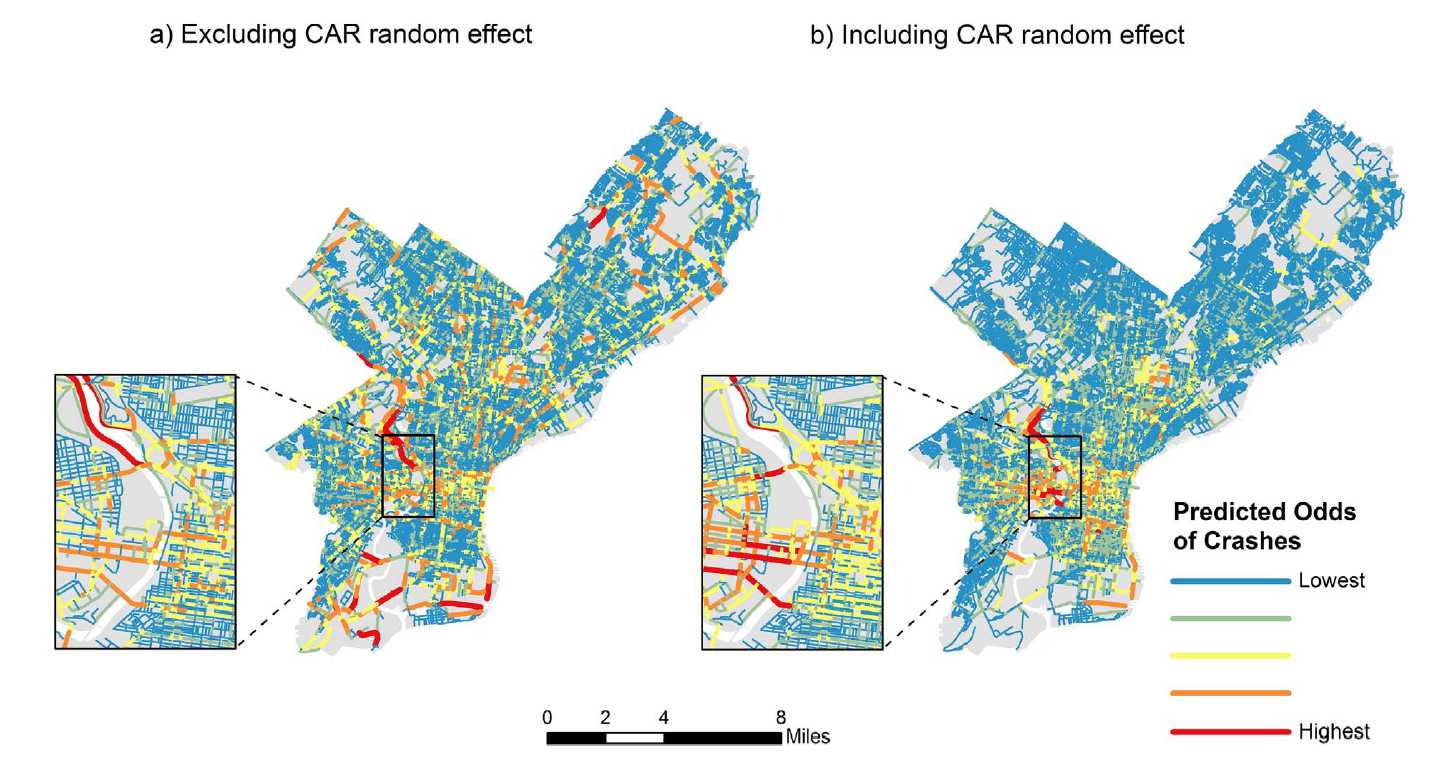
\includegraphics[width=\textwidth]{Plots/Kondor.png}
	\captionsource{(a und b). Berechnete Wahrscheinlichkeiten für Radunfälle in Philadelphia}{
		\cite{Kondo2018}
	}
	\label{kondor}
\end{figure}
Wie viele der bisher genannten Studien konzentrierte sich \cite{Kondo2018} auf eine Stadt, was ein nicht unwesentliches Problem darstellen kann, denn unterscheidet sich der Straßenverkehr von Stadt zu Stadt, wie auch \cite{Goldmann2021} zeigen. Gerade die Ergebnisse aus Philadelphia, einer der fahrradfreundlichsten Städte der USA, lassen sich eventuell nicht eins zu eins auf andere Städte der USA übertragen, da Autofahrer in Philadelphia durch den höheren Verkehr von Fahrrädern an die Rücksichtname gewöhnt sein könnten, die Autofahrer aus Erfahrung walten lassen. Deswegen wäre es ein interessanter Schritt, diese Beobachtungen auf einer Makro Ebene zu tätigen, um zu sehen, welche Faktoren Städte übergreifend für Fahrrad Sicherheit sorgen.\\
Genau dies machen \cite{Saha2018}, in dem Sie eine Analyse Floridas auf Zensus Block Größe vornehmen. Bei dieser Analyse stellen sie eine räumliche Konzentration und keine Gleichverteilung von Unfällen fest. Um dies zu erklären nutzen die Autoren ein bedingtes autoregressives Modell mit bedingten Variablen der Demographie, sozioökonimischen Daten, Straßen Infrastruktur und Radverkehr Charakteristiken. Davon wurden 21 Variablen als einflussreich identifiziert z.B. Bevölkerung, Alterskohorten, Autobesitz von Haushalten, Straßennetz Dichte oder Fahrradtour Intensität. Für das Modell worden Zensus Daten von 2011 bis 2014 verwendet, zu sehen auch in der Abbildung \ref{SAHA}.  
\begin{figure}[!ht]
	\centering
	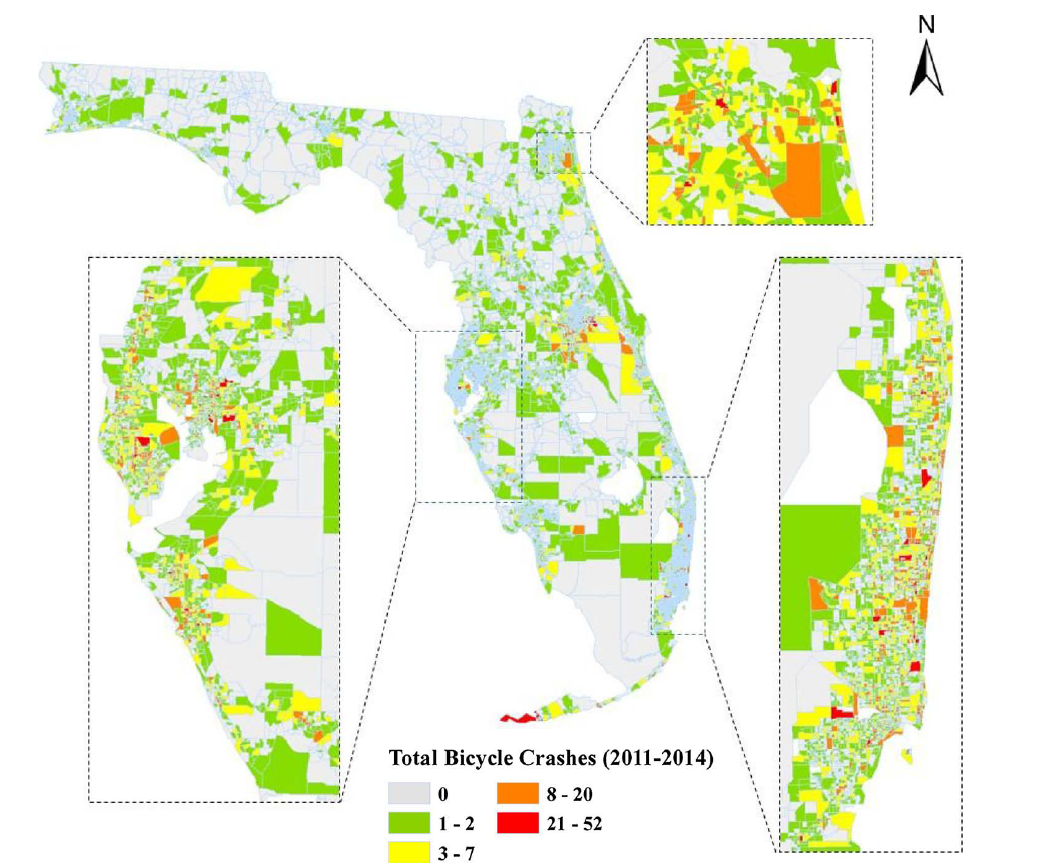
\includegraphics[width=\textwidth]{Plots/saha.png}
	\captionsource{Räumliche Verteilung aller Fahrradunfälle (2011–2014) nach Zensus Blöcken in Florida.}{
		\cite{Saha2018}
	}
	\label{SAHA}
\end{figure}
Gerade die letzten zwei Studien zeigen, wie interessant die räumliche Verteilung von Fahrradunfällen ist und \cite{Kondo2018} zeigen auch das Verkehrsvolumen als Faktor der Unfallwahrscheinlichkeit.\\
Neben all dem ist interessant, dass \cite{Kondo2018} darauf verweisen, dass Unfallsicherheit ein starker Prädikator sei für den Fahrradverkehr laut \cite{Pucher2010}, \cite{Thomas2013} und \cite{Winters2010}. Dies ist eine gute Überleitung auf das nächste Thema. Die bisherige Betrachtung beschäftigte sich mit den Daten, die man verwenden kann für die abhängige Variable des Modells, dass am Ende dieses Projekts entstehen soll. Doch für eine zuverlässige Vorhersage braucht es Prädikatoren. Diese sind in der Literatur zu finden.


\subsection{Sonstige Faktoren}

Eine weitere interessante Datenquelle, die wir z.B. schon bei \cite{Alattar2021} kennen gelernt haben, ist Open Street Map. Dies ist ein 2004 gegründetes gemeinnütziges Projekt, dass das Ziel verfolgt Kartenmaterial zu sammeln und online allen frei zur Verfügung zu stellen. Hier sind Daten über Straßen, Eisenbahnen, Flüsse, Wälder, Häuser und vielem weiteren zu finden. Auch \cite{Carl2015} nutzt die frei verfügbaren Daten zu Höhenmetern des Geländes von Open Street Map, um die Planung von mehrtägigen Fahrradtouren zu erleichtern, die der Erholung dienen. Deswegen ist dieses Paper für die Frage dieser Hausarbeit weniger interessant, die Idee, diese Art von Daten zu verwenden, aber könnte hilfreich sein. Dass aber die Topographie eine Rolle auch für den Pendler Verkehr spielt, zeigt \cite{Rietveld2004}.

\section{Forschungslücken und Anknüpfungspunkte}

Was die meisten der hier gezeigten Studien hier gemein haben, ist dass sie sich auf eine reine Zeitreihenanalyse beschränkt, jedoch die Daten nicht dazu nutzen die räumliche Verteilung der Daten zu untersuchen. Es gibt eine wenige Beispiele die das zwar tuen (Namen nennen), jedoch nie für den ganzen Verkehr, sondern nur für den Teil des Verkehrs, der im Rahmen von Leihradsystemen geschieht. Auch die Kontrolle der Routenwahl durch GPS Tracking, stellt immer nur einen verzerrten Teil des gesamten Verkehrs da, entweder durch zu geringe Stichprobengößen oder durch die Selbstselektion der Studienteilnehmer.\\
Das lässt nur die Forschung übrig, die mit Daten von Zählstationen rechnet. Diese verfolgt aber meist das Ziel kausale Einflüsse auf den Radverkehr zu untersuchen wie bei (...). Andere Studien treffen zwar Vorhersagen, aber eben nicht in eine räumliche Dimension hinein, wie bei (Holmgren). Die Forschungsfrage dieser Masterarbeit erfordert aber eine räumliche Interpolation, um Vorhersagen für ein gesamtes Stadtgebiet zu treffen und nicht über einzelne Stationen, die vorher so beobachtet worden. Eine kausale Interpretation ist hierfür nicht zwangsläufig notwendig, wenn auch interessant. Außerdem würde eine kausale Interpretation die Verwendung von neuronalen Netzwerken ausschließen.\\
Nur wenige Studien untersuchen die Daten mehr als einer Stadt, mit ausnahme von (...). Aber die Verwendung von mehreren Städten wäre zwingend notwendig. Denn wie man im Vergleich sieht, bieten Studien mit Radzählstellen oft weniger Beobachtungspunkte pro Stadt, als z.B. Studien die GPS Tracking Daten verwenden oder Daten von Leihsystemen. Um diesen Nachteil auszugleichen, ist es ratsam, Daten mehrere Städte zu verwenden. Die Studie von ... zeigte, wie man die Unterschiede zwischen Städten hervor heben kann ist. So ist es ratsam demographische und soziale Daten über die Stadtstrukturen in einen Datensatz mit aufzunehmen. Bei ... zeigten diese Daten Unterschiede in der Wetterelastizität des Fahrradverkehrs auf. In dieser Studie würden die stadtbezogenen Daten Unterschiede im Radverkehr selbst kenntlich machen.\\
Zueletzt erfordert die Forschungsfrage Stationsbasierte Daten, möchte man Unterschiede im Radverkehrsaufkommen innerhalb der selben Stadt erkennen und auch vorhersagen können. Nur daraus ergeben sich räumliche Unterschiede im Stadtbild. Eine Studie, dient hier zB als Vorbild, in dem sie Daten von POIs in Google Streetview verwendet. ... Verwenden hierbei Bilderkennung. Soweit würde diese Masterarbeit nicht gehen. Allerdings könnte man Entfernung von Zählstationen und einigen POIs im Stadtbild mit in das Modell aufnehmen. Dies allgemein gibt einen guten Ausblick auf das kommende Kapitel im Allgemeinen. Anhand der bestehenden Literatur ließ sich festmachen, welche Datenstruktur notwendig ist, um die Forschungsfrage zu beantworten. Das kommende Kapitel gibt einen Einblick in den endgültigen Datensatz.

\chapter{Zusammensetzung des Datensatz}\label{Datensatz}

Das vorherige Kapital zeigte den aktuellen Stand der Forschung zum Aufkommen des Fahrradverkehrs und endete mit einer Einschätzung, an welchen Studien sich diese Masterarbeit orientieren muss, um die gestellte Forschungsfrage zu beantworten. Darauf baute auch die Beschaffung von Daten für das Modell dieser Arbeit auf, angefangen über die Daten der Fahrradzähler, Daten zum Wetter, demographischen Daten und Daten der vorhandenen Infrastruktur erhoben durch Open Street Map und dazu gehörigen Points of Interest. Einen tieferen Einblick über die Datenbeschaffung und die Verteilung von Daten mit zugehörigen Abbildung beinhaltet dieses Kapitel.\\
Die Datenbeschaffung an sich beschränkt sich allein auf Deutschland aus Gründen der Einfachheit. Bestimmte Daten wie Daten zum Wetter und zur Demographie lassen sich so allein von einer Datenquelle beschaffen in diesem Fall dem Deutschen Wetter Dienst und dem statistischen Bumdesamt DESTATIS. Der Nachteil davon ist, dass wiederum alle Aussagen des Modells allein für Deutschland gültig sind, da dieser Rahmen die Evaluierung für andere Regionen der Welt nicht zu lässt.

\section{Fahrradzähler}

Notwendige Grundlage der Forschung sind Daten von Fahrradzählstationen. Dankbarerweise stellen diese Daten viele Kommunen öffentlich zur Verfügung oder teilen diese auf Nachfrage. In welchen Städten sich Fahrradzähler finden ließen, die in das Modell aufgenommen werden konnten, zeigt die Abbildung \ref{Deutschlandkarte}. Alle Fahrraddaten sind stündlich aufgelöst. D.h. die Anzahl der Fahrradfahrer, die eine Zählstation passierten, wurde innerhalb einer vollen Stunde aufsummiert.
\begin{figure}[!ht]
	\centering
	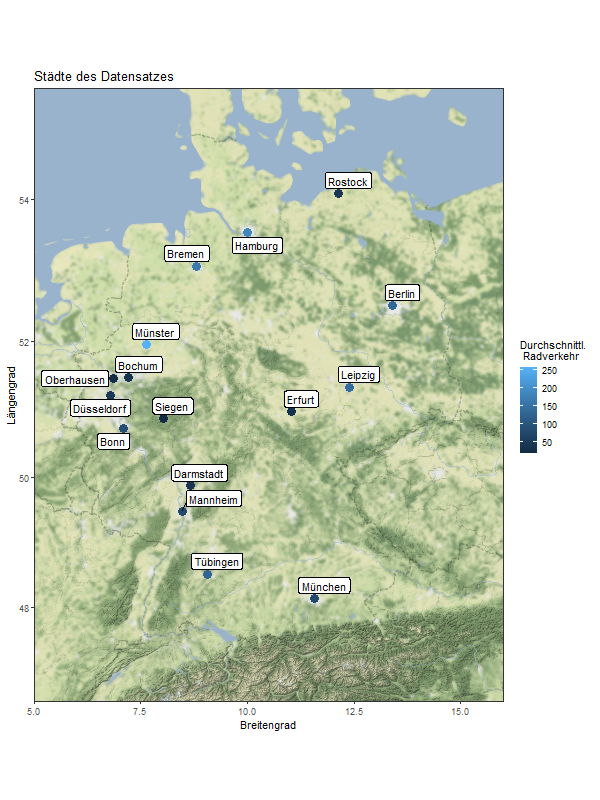
\includegraphics[width=\textwidth]{Plots/plot22.png}
	\caption{Städte die im Datensatz vertreten sind.}
	\label{Deutschlandkarte}
\end{figure}

Ein grundsätzliches Problem des Datensatzes, dass sich so leicht auch nicht beheben lässt, dass zum einem Großstädte mehr Fahrradzähler errichten, zum anderem ihre Daten oft auch leichter zugänglich machen. Die Abbildung \ref{Einwohnergroese} zeigt deutlich, dass Großstädte mit mehr als 300 Tsd Einwohnern im Datensatz überrepräsentiert sind. Deshalb sollte man bei Vorhersagen für Städte mit weniger als 300 Tsd Einwohnern vorsichtig in der Interpretation sein.

\begin{figure}[!ht]
	\centering
	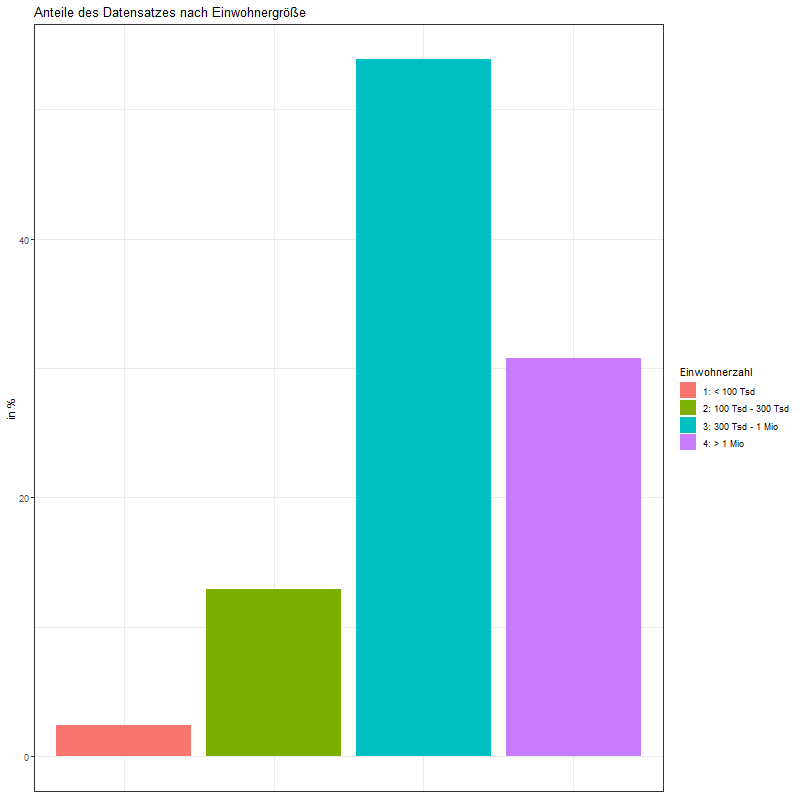
\includegraphics[width=\textwidth]{Plots/plot10.png}
	\caption{Verteilung der Beobachtung nach Einwohnergröße der Städte}
	\label{Einwohnergroese}
\end{figure}

Die Datenquelle sind die Kommunen selbst. Eine Veröffentlichung aller Daten ist dabei nicht möglich, weil die Kommunen unterschiedliche Bedingungen für die Verwendung der Daten gestellt haben. Der Betrachtungszeitraum der Daten reicht von 2012 bis 2022 in einigen Fällen. Einige wenige Zählstellen in Hamburg und Siegen wurden erst 2022 aufgestellt. In allen anderen Städten reichen die Beobachtungen aber nur bis 2021. Die Abbildungen \ref{Jahre} zeigt wie sich die Daten über die Zeit verteilen. Dabei ist festzustellen, dass je weiter wir in die Vergangenheit gehen, desto weniger Daten finden wir, da nur wenige Zählstationen seit 2012 im Betrieb sind. (An dieser Stelle könnte man noch über die Fahrradzähler in Hamburg schreiben)

\begin{figure}[!ht]
	\centering
	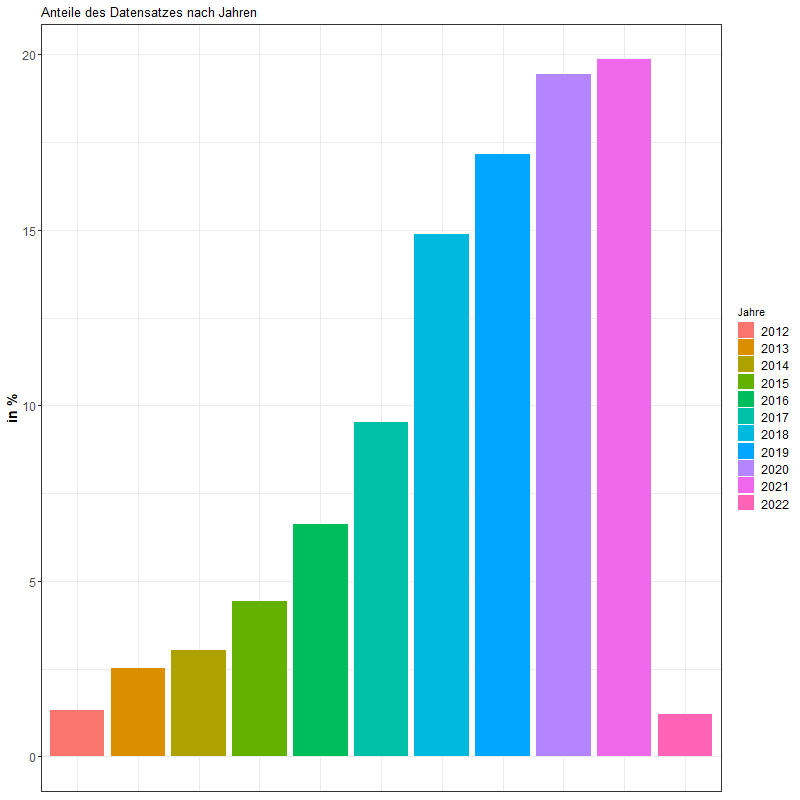
\includegraphics[width=\textwidth]{Plots/plot28.png}
	\caption{Verteilung der Beobachtung nach Jahren}
	\label{Jahre}
\end{figure}

\section{Wetterdaten}

Daten zum Wetter stammen einheitlich vom Deutschen Wetterdienst. Dabei wurden die Fahrraddaten einer Stadt immer mit den Wetterdaten der nächstgelegenen Stadt verwendet. Nur Mannheim und Heidelberg teilen sich die Daten einer Wetterstation, da beide Städte sehr nah beieinander liegen. Insgesamt wurden Daten in den Datensatz mit aufgenommen zum Niederschlag in mm, zur Lufttemperatur in 2 m Höhe in Grad Celsius, zur Wolkenbedeckung in Achteln, zur relativen Feuchte in \% und zur durchschnittlichen Windgeschwindigkeit. Genau wie die Fahrraddaten sind die Wetterdaten stündlich aufgelöst. Einen jährlichen Durchschnittsverlauf über alle Daten zeigt Abbildung \ref{fig:TempNied}a. Weiterhin zeigt die Abbildung \ref{fig:TempNied}b den Zusammenhang zwischen Radfahrer und Monatstemperaturen.

\begin{figure}%
	\centering
	\subfloat[\centering Temperatur und Niederschlag]{{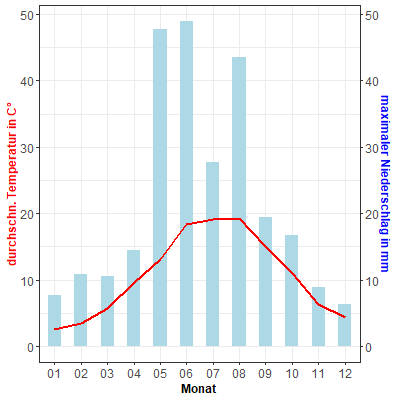
\includegraphics[width=6cm]{Plots/plot23.png} }}%
	\qquad
	\subfloat[\centering Temperatur und Radfahrer]{{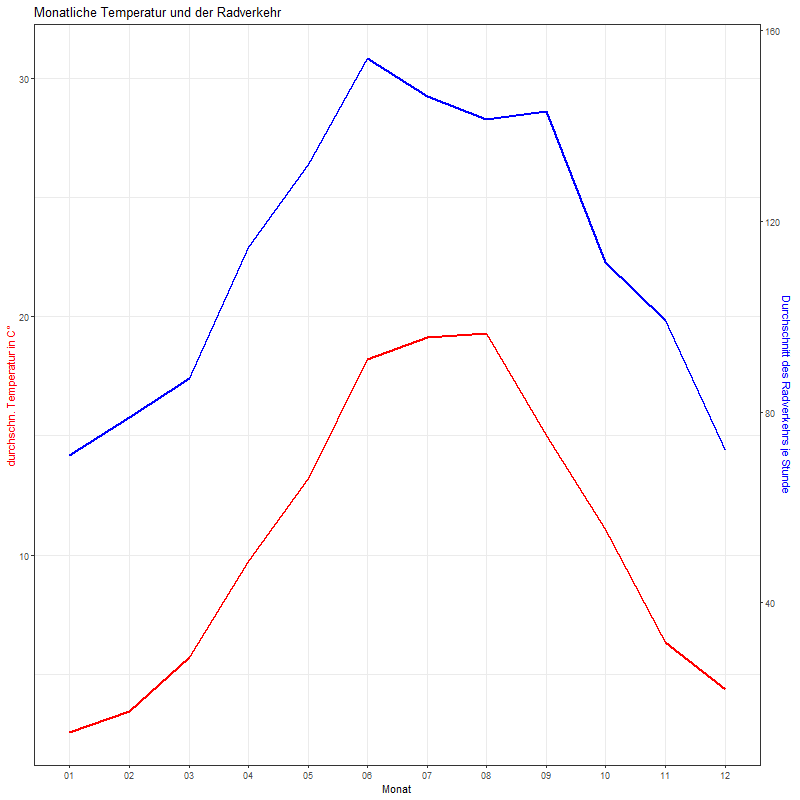
\includegraphics[width=6cm]{Plots/plot24.png} }}%
	\caption{Wettterdaten im Überblick}%
	\label{fig:TempNied}%
\end{figure}


\section{Demographische und soziale Statistiken}\label{Daten_Stadt}

In diesem Abschnitt sammeln sich verschiedene Daten, die Unterschiede in den Städten in ihrer sozialen und demographischen Struktur in ihrer Bevölkerung hervorheben. Daten dafür stammen aus zwei Quellen. Die meisten Variablen nutzen als Datenquelle das statistische Bundesamt. Eine Variable bezieht sich auf den ADFC Fahrradklimaindex. Für beide Quellen gilt, dass Daten für das Jahr 2022 noch nicht vorhanden waren, da das Jahr zum Zeitpunkt der Recherche noch nicht abgeschlossen war. Für die wenigen Beobachtungen aus Hamburg z.B., die aus dem Jahr 2022 in den Datensatz mit aufgenommen worden sind, gilt, dass für diese Beobachtungen angenommen wurde, dass Variablen, die nicht erneuert werden konnten, konstant blieben. Das betrifft insgesamt jedoch nur wenige Beobachtungen, wie auch Abbildung \ref{Jahre} zeigt.

\subsection{Statistisches Bundesamt}

Das statistische Bundesamt, stellt verschiedene Tabellen zur Verfügung, die wertvolle Einblicke in die Unterschiede der Gemeinden geben, in denen sich die verschiedenen Fahrradzählstationen befinden.\\

\begin{figure}%
	\centering
	\subfloat[\centering Radverkehr nach Bevölkerungsgröße]{{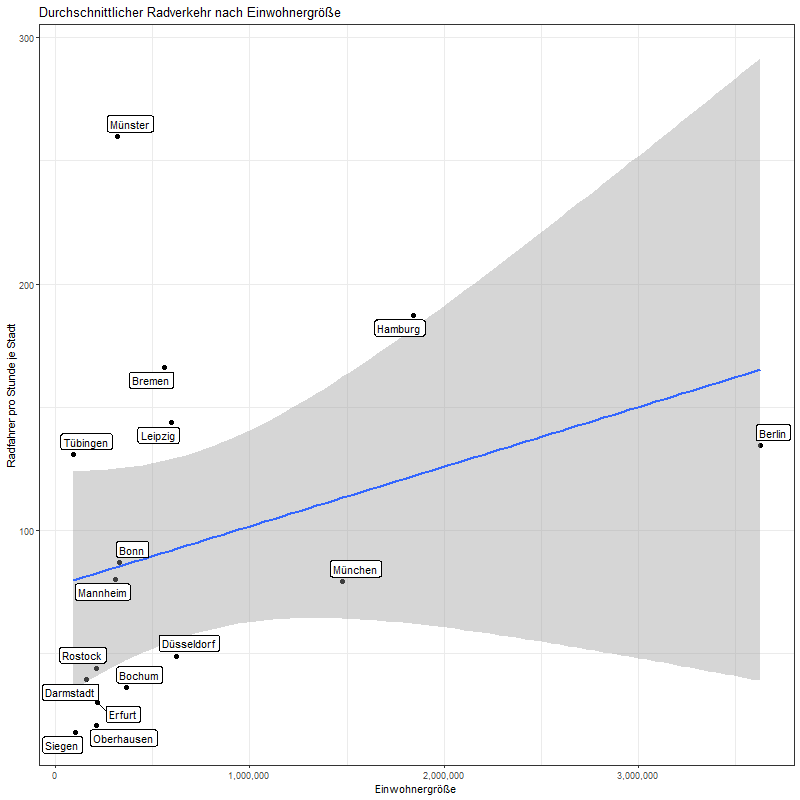
\includegraphics[width=6cm]{Plots/plot01.png} }}%
	\qquad
	\subfloat[\centering Radverkehr nach Anteil der männl. Bev.]{{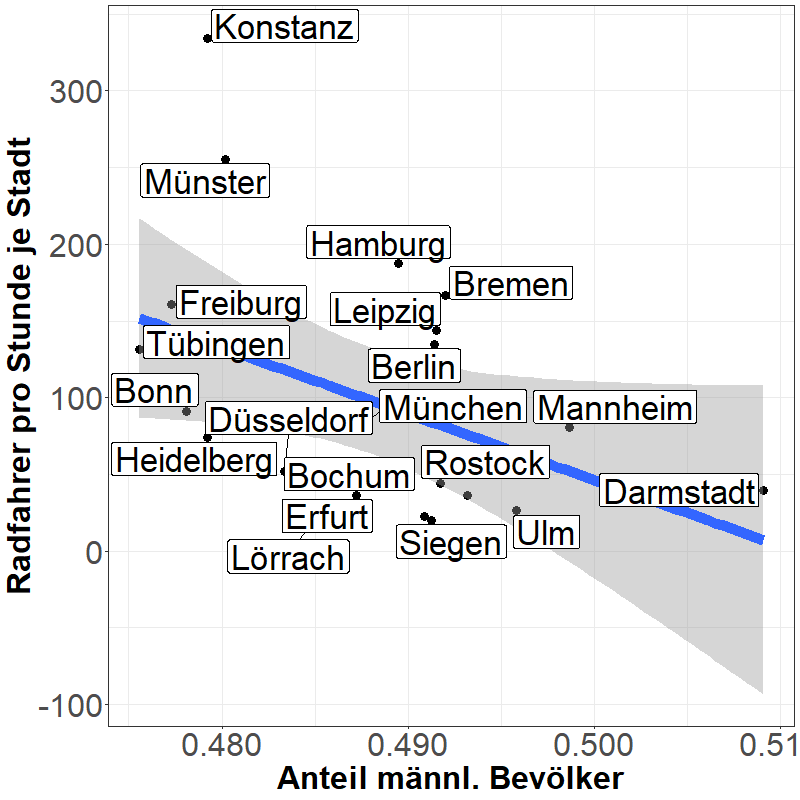
\includegraphics[width=6cm]{Plots/plot02.png} }}%
	\caption{Verhältnis von Bevölkerung und Fahrradaufkommen}%
	\label{fig:Gemeindevz}%
\end{figure}

Eine wichtige grundlegende Quelle ist das Gemeindeverzeichnis für alle politisch selbständigen Gemeinden (mit Gemeindeverband) in Deutschland, das jedes Jahr veröffentlicht wird. Dieses Verzeichnis beinhaltet nicht nur Landkreise und kreisfreie Städte, sondern hält auch Zahlen zu jeder Gemeinde bereit. Dabei sind Daten zur Fläche in km², zur Einwohneranzahl, sowohl männlich, weiblich wie auch insgesamt vorhanden. Diese fanden auch ihren Weg ins Modell. Wie sich Einwohnergröße und der Anteil an Männern in der Bevölkerung zum Aufkommen an Fahrradfahrern verhalten, kann man in der Abbildung \ref{fig:Gemeindevz} sehen. Außerdem verwendet das Modell die angegebenen Längen- und Breitengrade, aus denen der jeweilige Abstand der Farradzählstation zum Stadtzentrum berechnet wird, auch dargestellt in Abbildung \ref{Stadtzentrum}. Das Modell greift dabei auf das Gemeindeverzeichnis von 2012 bis 2021 zurück.\\

\begin{figure}[!ht]
	\centering
	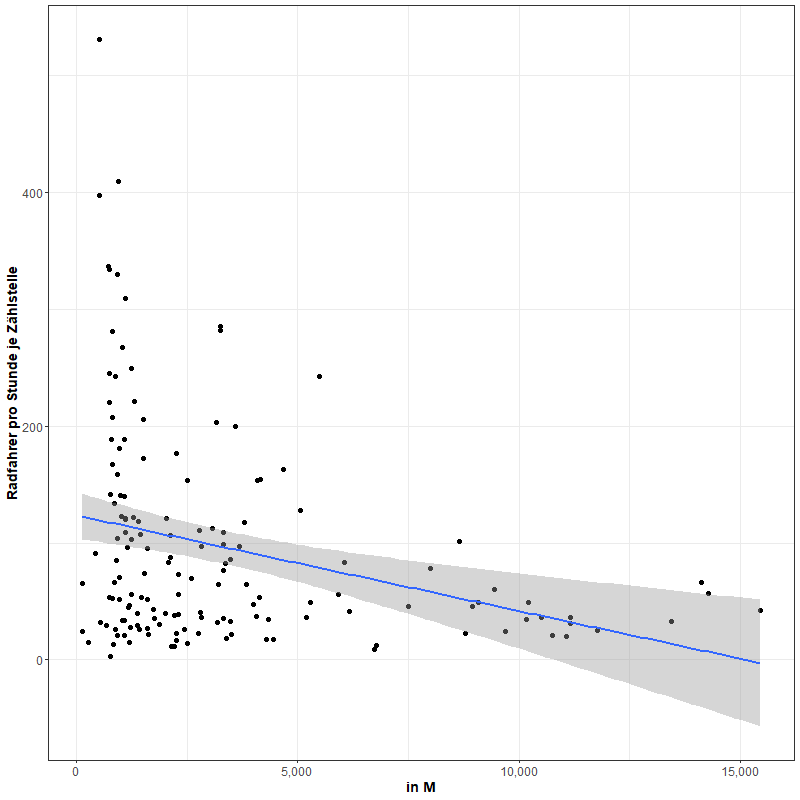
\includegraphics[width=\textwidth]{Plots/plot11.png}
	\caption{Verteilung des Fahrradaufkommens in Entfernung zum Stadtzentrum}
	\label{Stadtzentrum}
\end{figure}

Weitere Daten zur demographischen Verteilund der Bevölkerung in den jeweils betroffenen Landkreisen und kreisfreien Städten stammen aus der Tabelle 12411-0017 zur Bevölkerung nach Kreisen, Stichtag, Altersgruppen von \cite{Destatis2022_a}. Mit diesen Daten ließ sich der Anteil der Bevölkerung berechnen, der jünger als 18, 25, 30 und älter als 40 und 60 ist. Wie sich das Radverkehrsaufkommen zum Anteil der Bevölkerung unter 30 verhält nach Städten zeigt auch die Abbildung \ref{Alter} im Anhang.

Auch eine wertvolle Statistik bietet die Tabelle 46251-0020 über den Kraftfahrzeugbestand nach Kreisen, Stichtag, Kraftfahrzeugarten von \cite{Destatis2022b}. Mithilfe der Einwohneranzahl je Kreis ließ sich die Quote an Kraftfahrzeugen je Person berechnen. Außerdem zeigt die Tabelle 12521-0040 über die Anzahl der Ausländer nach Kreisen, Stichtag und Geschlecht von \cite{Destatis2022c} ebenfalls wichtige Einblicke zu sehen in Abbildung \ref{fig:PKSundAusl}.

\begin{figure}[!ht]%
	\centering
	\subfloat[\centering Radverkehr nach PKWs je Person]{{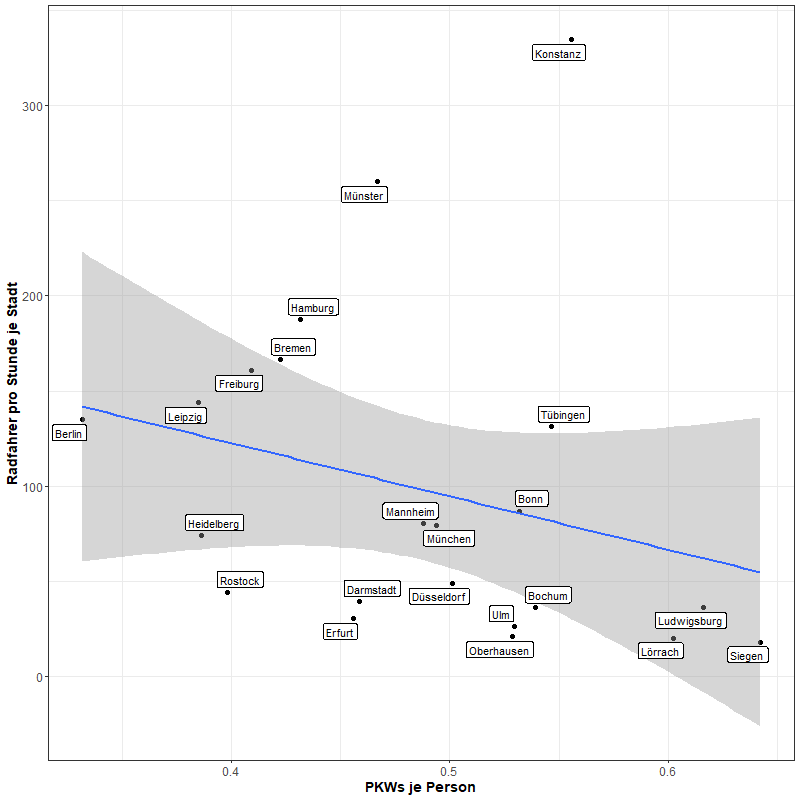
\includegraphics[width=6cm]{Plots/plot06.png} }}%
	\qquad
	\subfloat[\centering Radverkehr nach Immigrantenanteil]{{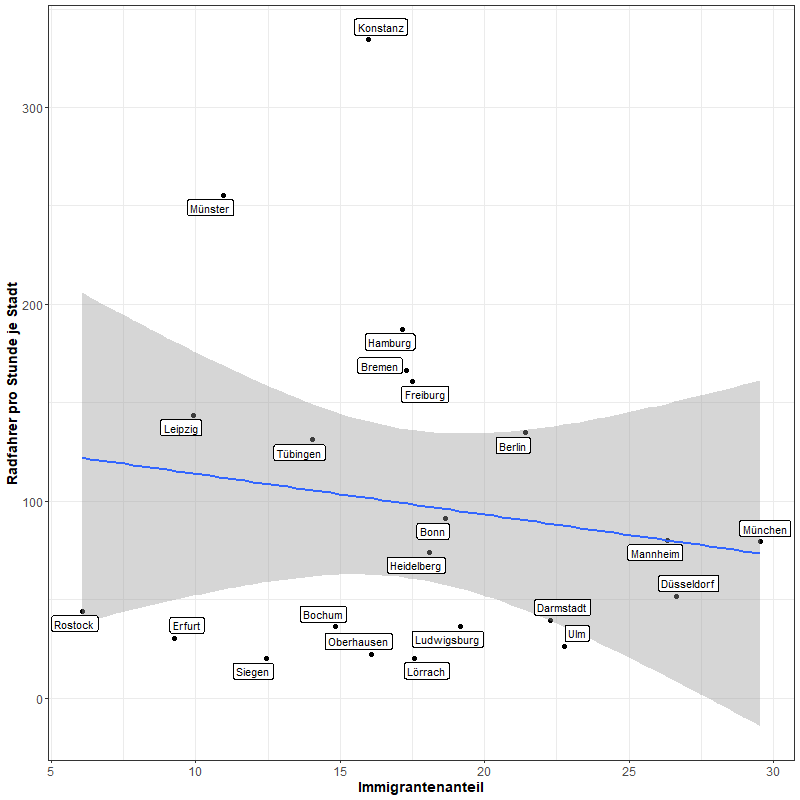
\includegraphics[width=6cm]{Plots/plot07.png} }}%
	\caption{Verhältnis von Bevölkerung und Fahrradaufkommen}%
	\label{fig:PKSundAusl}%
\end{figure}

\subsection{ADFC Fahrradindex}

Neben den stadtspezifischen Daten, die von den Quellen des statistischen Bundesamtes stammen, nutzt der Datensatz die Daten zum ADFC Fahrradklimaindex. Der Allgemeiner Deutscher Fahrrad-Club ist ein eingetragener Verein mit Sitz in Berlin und Bremen, der sich für die Interessen von Fahrradfahrern einsetzt und stand 2022 220.000 Mitglieder in Deutschland zählt. Im Zweijahresrhytmus veröffentlicht der ADFC den per Umfrage ermittelten Fahrradklimaindex. 2022 wurden z.B. 238 Tsd Menschen befragt aus verschiedenen Städten. Neben Fragen zum persönlichen Fahrradfahren enthält der Fragebogen zum Fahrradklima Index Fragen betreffend des Fahrradklimas, dem Stellenwert des Radverkehrs in der jeweiligen Stadt, der Sicherheit, dem Komfort und der Infrastruktur sowie der Radverkehrsnetze. All diese Antworten fließen in eine Endnote, die sich zwischen 1 und 5 befindet, wobei 1 am Besten und 5 am schlechtesten ist. Wie sich das Fahrradklima ins Verhältnis zum aufgezeichneten Radverkehr ins Verhältnis nach Städten setzt, zeigt die Abbildung \ref{Fahrradklima} im Anhang.

\section{Corona Daten}

Wie \cite{Moellers2021} bereits zeigten, hatten die Corona Maßnahmen unterschiedliche und nicht ganz eindeutige Auswirkungen auf den urbanen Radverkehr. Dennoch ist es ratsam, Variablen in das Modell mitaufzunehmen, die Ausprägung von Corona Maßnahmen berücksichtigen. Wie bei \cite{Moellers2021} ließen sich dafür die Corona Inzidenzzahlen verwenden, oder aber eine Dummy Variable für Lockdowns.\\
Bei beiden Ansätzen stellen sich Probleme ein. War die Corona Inzidenz zu Beginn recht klein, waren die Auswirkungen für den Verkehr dennoch drastisch. Die Abbildung \ref{CoronaInzidenz} gibt darüber einen Überblick. Deswegen beinhaltet der Datensatz zusätzlich eine Dummy Variable für die zwei bundsweiten Corona Lockdowns vom 22.3.2020 bis zum 4.5.2020 und vom 2.11.2020 bis zum 14.2.2020. In diese Zeitphasnen fallen verschiedene Maßnahmen zur Kontaktbeschränkung, die jeweils bundesweit stattgefunden haben. Dabei kann es regional zu Abweichungen kommen, die sich im Nachhinein nicht ohne immensen Aufwand nachvollziehen lassen.

\begin{figure}[!ht]
	\centering
	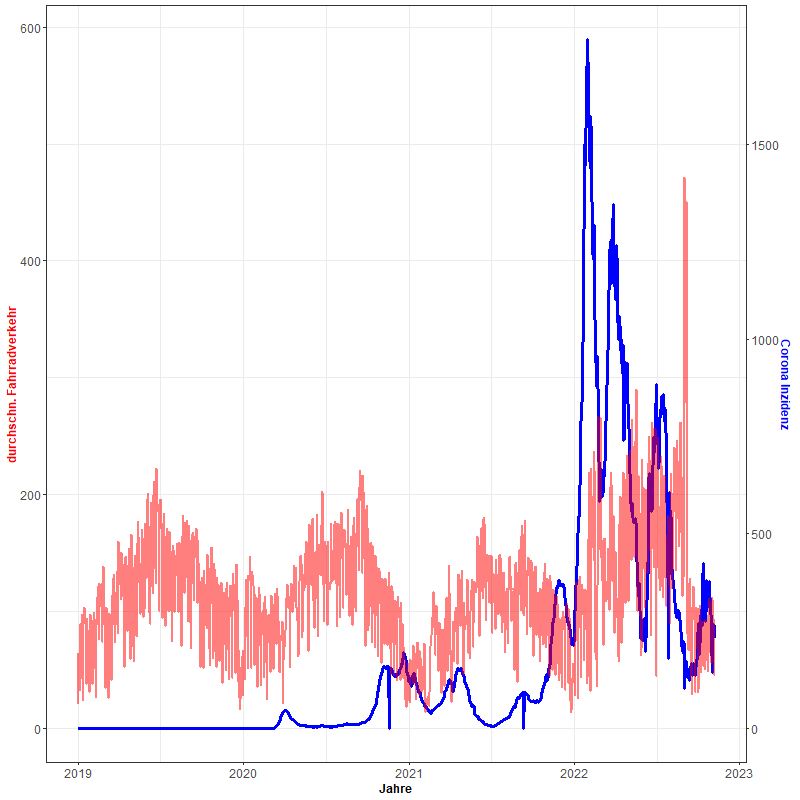
\includegraphics[width=\textwidth]{Plots/plot62.png}
	\caption{Verlauf der Corona Inzidenz und des Radverkehrs}
	\label{CoronaInzidenz}
\end{figure}

Diese Schwäche sollen die Daten zur Corona Inzidenz ausgleichen, die lokal mit Maßnahmen zur Kontaktbeschränkung korrelieren. Die Daten dazu stammen vom Robert Koch Institut (Quelle: \url{https://www.rki.de/DE/Content/InfAZ/N/Neuartiges_Coronavirus/Daten/Inzidenz-Tabellen.html?nn=2386228}). Leider reichen die Daten des RKIs nicht für alle einzelnen Kommunen bis zum Beginn der Pandemie zurück. Im Zeitraum 10.3.2020 bis zum 6.5.2020 sind die im Datensatz enthaltenen Daten zur Corona Inzidenz bundesweit. Danach und bis zum 18.11.2020 verwendetet der Datensatz die Inzidenzen der jeweiligen Bundesländer. Erst danach sind die Inzidenzen der jeweiligen Landkreise und die der kreisfreien Städte verfügbar.\\
Bei der ersten Erstellung des Datensatz, waren die Corona Daten leider noch nicht mit inbegriffen und erste Modelle wurden ohne diese Daten berechnet. Daraufhin wurde ein zweiter Datensatz erstellt, der nicht nur die Corona Daten zusätzlich berücksichtigte, sondern auch neuere Daten zu Straßen anlegte, dazu mehr im Detail im folgenden Abschnitt. Im weiteren Verlauf des Textes wird kenntlich gemacht, mit welcher Version des Datensatzes Berechnungen gemacht wird, ob mit der alten ohne Corona Daten oder der neuen mit Corona Daten.\\

\begin{figure}[!ht]
	\centering
	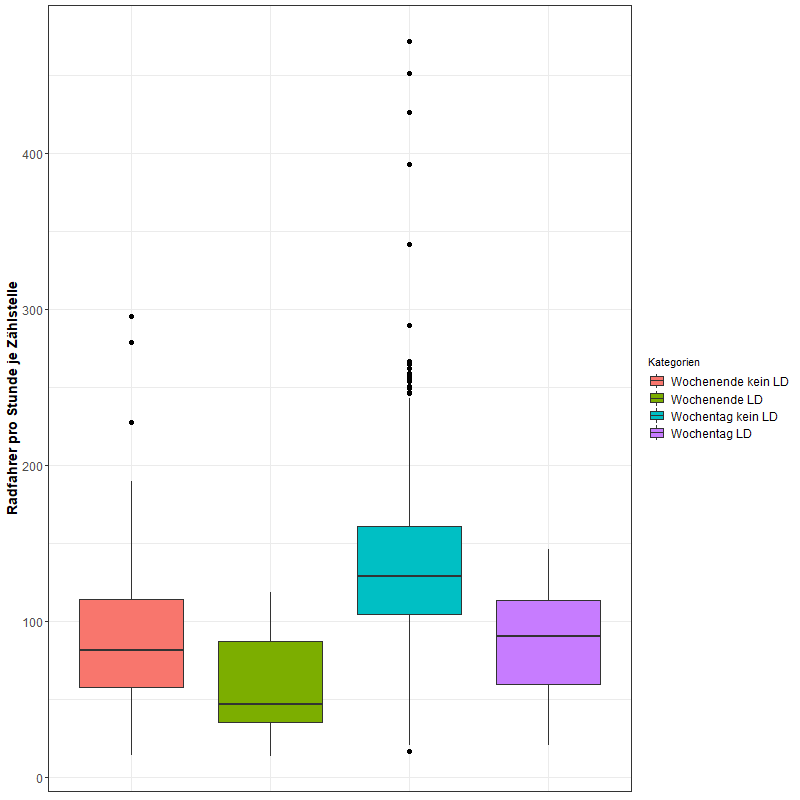
\includegraphics[width=\textwidth]{Plots/plot63.png}
	\caption{Radverkehr im Lockdown}
	\label{CoronaandBiking}
\end{figure}

Anders als bei \cite{Moellers2021} gibt es in dem neuen Datensatz kein zwiespältigen Effekt, wie die Abbildung \ref{CoronaandBiking} zeigt. Sowohl am Wochenende, als auch unter der Woche ist das Aufkommen des städtischen Radverkehrs gesunken.



\section{Open Street Map Daten}\label{OMSDATA}

Im vorherigen Abschnitt wurden die Datenquellen zu stadtspezifischen Daten erläutert. Variablen zur demographie oder dem Autobesitz nach Städten sind wertvoll, um die Unterschiede im Radverkehr zwischen den Städten einschätzen zu können. Dies hilft jedoch nicht bei der räumlichen Unterscheidung. Verwendet man keine räumlichen Merkmale, so erhält man eine einheitliche Vorhersage je Stadt. Die räumliche Verteilung des Radverkehrs innerhalb jeder Stadt, ließe sich so nicht abbilden. Die einzige räumliche Variable, die bisher erhoben wurde, ist die Entfernung zum Stadtzentrum, beruhend auf den Daten des Gemeindeverzeichnis von 2012 bis 2021. Doch selbst mit dieser Variablen, gingen Abweichungen durch lokale Anlaufpunkte wie bei Bahnhöfen verloren.\\
Der daraus resultierende Schluss ist, Koordinaten zu solchen Anlaufpunkten oder auch Points of Interest (PoIs) dazu zu nutzen, Entfernungen zu den Radzählstationen zu berechnen, und die Anzahl nach Radius und Entfernung zum nächstgelegenen PoI mit in das Modell aufzunehmen. Die beste Datenquelle hierfür bietet Open Street Map (OMS). Wie schon im Kapitel \ref{Faktor_Stadt} beschrieben, handelt es sich bein Open Street Map um ein internationales Projekt, das in gemeinsamer Freiwilligenarbeit geographische Daten sammelt und öffentlich zur Verfügung stellt.\\

\begin{lstlisting}[caption={OSM Daten Abfrage},label=code:osmdata_query]
q <- getbb(toString(rawData$Town[1])) %>%
opq() %>%
add_osm_feature("amenity", "cinema")
	
cinema <- osmdata_sf(q)
\end{lstlisting}

Der Zugriff auf die OSM Daten funktioniert mit dem R-Paket \glqq osmdata\grqq von \cite{Padgham2017}. Dieses Paket bietet die Möglichkeit Daten verschiedener OSM Kategorien abzufragen über den Code \ref{code:osmdata_query}. Dabei bezeichnet \lstinline|rawData$Town[1]| den ersten Eintrag in der Variable \lstinline|Town| für den Grunddatensatz \lstinline|rawData|. Da jede Stadt ihr eigenes Skript hat, ist dies jeweils die relevante Stadt. Für diese Stadt wird eine Anfrage gestellt, die bestimmte Features erfüllen muss. Im Code Beispiel werden Kinos gesucht. Mithilfe des R-Pakets \glqq sf\grqq von \cite{Pebesma2018} werden die Daten der Anfrage in ein simple Feature Format gespeichert in \lstinline|cinema|. Dieses Format beinhaltet Koordinatenpunkten, mit jeweiliger ID und teils Namen und Adressen der verschiedenen Einrichtungen. Darüber hinaus aber auch Koordinaten der Linien, falls es sich z.B. um Straßennetze handelt, oder Koordinaten der jeweiligen Polygone der Gebäudegrundrisse.


\subsection{Ausgewählte PoIs}

Dieser öffentliche Zugang zu kategographischen Daten beinhaltet nicht nur Straßenverläufe, sondern auch Lageparameter zur öffentlichen Einrichtungen, Geschäften, Verkehrsknotenpunkten von Bus und Bahn, Ampeln und Straßenübergängen und vielem mehr. Es gibt also eine große Auswahl an Kategorien, die sich in das Modell aufnehmen ließen. Die Auswahl begrenzte sich dabei auf Kinos, Schulen, Universitätsgebäuden, Supermärkten, Kleidungsgeschäften und Fahrradwerkstätten. Die Auswahl dessen fand rein intuitiv statt. Schüler und Studenten sind häufiger Fahrradfahrer als der Rest der Bevölkerung. Kleidungsgeschäfte sind oft räumlich stark konzentriert im Stadtzentrum und bildern hierfür einen guten Indikator. Hat eine Stadt ein hohes Angebot an Fahrradwerkstätten, ist dies ein guter Hinweis darauf, dass hier ein hoher Radverkehr zu finden ist. Die Auswahl von Kinos und Supermärkten ist rein zufällig.\\

Noch empfehlenswert wäre es den Datensatz um noch mehr Kategorien zu erweitern und genau zu evaluieren, welche Kategorien die Performance des Modells erhöhen. Jedoch hätte dies den Arbeitsumfang dieser Masterarbeit nochmals drastisch erhöht. In Abwägung des zeitlichen Aufwands und dem Nutzen für das Modell, beschränkt sich deswegen der Datensatz auf die erwähnten PoI's.\\
In jeder Kategorie wurde jeweils die Entfernung der jeweiligen Radzählstation zum jeweiligen PoI berechnet. Darüber hinaus wurden in jeder Kategorie die Anzahl an Einreichtungen in zwei verschiedenen Radien berechnet. Für Kinos und Fahrradwerkstätten wurde ein ein Kilometer und ein drei Kilometer Radius gewählt. Für Schulen, Universitätsgebäude und Kleidungsgeschäfte wurde ein 500 Meter und ein zwei Kilometer Radius gewählt. Für Supermärkte wurde ein 500 Meter und ein ein Kilometer Radius genutzt. Die Auswahl dieser Berechnungsgrenzen sind wiederum rein zufällig. Eine genaue Evaluation dieser Auswahl fand nicht statt. Zu Universitätgebäuden, Supermärkten und Kleidungsgeschäften finden sich die Abbildungen \ref{UniBuild}, \ref{SuperMarket} und \ref{ClothesShop} im Anhang. Für Städte, die über keine Universität verfügen, wurde angenommen, dass die nächste Universität mindestens 50 km weit entfernt sei.

\begin{lstlisting}[caption={Speichere die OSM Koordinaten},label=code:matrix]
cinmat=matrix(1:3*length(cinema$osm_polygons$osm_id), 
	nrow = length(cinema$osm_polygons$osm_id), 
	ncol = 3)
	
for(i in 1:length(cinema$osm_points$name)){
   	cinmat[i,1]=cinema$osm_polygons$osm_id[i]
	cinmat[i,2]=as.data.frame(
		cinema$osm_polygons$
		geometry[[i]][1])[1,1]
	cinmat[i,3]=as.data.frame(
		cinema$osm_polygons$
		geometry[[i]][1])[1,2]
}
\end{lstlisting}

Der Code \ref{code:matrix} zeigt die Umwandlung der Daten. Von Interesse sind nur die ersten Koordinatenpunkte der jeweiligen Polygone der Kinogebäude. Dazu wird die Matrix \lstinline|cinmat| erstellt, die 3 Spalten hat und deren Reihenanzahl der Anzahl an ID's sind \lstinline|length(cinema$osm_polygons$osm_id)| entspricht, damit in diesem Fall alle Kinos berücksichtigt werden. Mittels einem \lstinline|for|-Loop werden alle Daten eingespeichert, so der Längengrad und Breitengrad in \lstinline|cinema$osm_polygons$geometry[[i]][1])[1,]|, der  und die jeweilige ID in \lstinline|cinema$osm_polygons$osm_id[i]|. Diese Matrix wird danach in ein Dataframe umgewandelt, um damit einfacher arbeiten zu können.\\

Nun muss nur noch für jede einzelne Zählstation die jeweilige Distanz zu den verschiedenen Kinos berechnet werden. Dazu bietet das R-Paket \glqq geosphere\grqq von \cite{Hijmans2021} die Funktion \lstinline|distm|, mit deren Hilfe man mit zwei Koordination die Entfernung in Metern berechnen lassen kann. Pro Zählstation wird der \lstinline|For|-Loop im Code \ref{code:distc} ausgeführt. Im code sind zwei Indexnummern zu finden, dabei steht i für die jeweilige Zählstation und j für das jeweilige Kino. Im dataframe d sind die Koordinaten der jeweiligen Zählstationen gespeichert. Zusammen mit den Koordinaten der Kino im cinmat Datenframe kann die Funktion distm die Entfernung beider Koordinaten zueinander berechnen. Diese Entfernung wird dann im Vector distc gespeichert.

\begin{lstlisting}[caption={Berechnung der Entfernung},label=code:distc]
for (j in 1:length(cinmat$id)) {
	cindist=distm(c(d$Lon[i],d$Lat[i]),
		c(cinmat$lon[j],cinmat$lat[j]), 
		fun=distGeo)
	distc[j]=cindist
}
\end{lstlisting}

Nun ist ein Vector vorhanden der alle Entfernungen gespeichert hat. Dieser kann nun dazu genutzt werden die benötigten Variablen zu berechnen. Zusammen mit dem Namen der aktuellen Station, der im Subset Datensatz \lstinline|d[1,1]| zu finden ist wird die jeweilige Variable gespeichert. Dabei lässt sich mit der Funktion \lstinline|min(distc)| die Entfernung zum nächstgelegenen Kino finden. Die Anzahl an Kinos in einem 1 km Radius findet sich mit der Funktion \lstinline|sum(distc < 1000)|.

\begin{lstlisting}[caption={Berechnung der Entfernungsvariablen},label=code:dist_variables]
distmat_closest[i,1]=d[1,1]
distmat_closest[i,2]=min(distc)

distmat_1kmradius[i,1]=d[1,1]
distmat_1kmradius[i,2]=sum(distc < 1000)
\end{lstlisting}

Die so berechnet Variablen lassen sich einfach verbinden mit dem Befehl \lstinline|merge|.

\begin{lstlisting}[caption={Füge neue Variablen dem Datensatz hinzu},label=code:dist_variables2]
rawData = merge(x = rawData,y = distmat_closest,
by = c("Station"),
all = FALSE)

rawData = merge(x = rawData,y = distmat_1kmradius,
by = c("Station"),
all = FALSE)
\end{lstlisting}

\subsection{Ausgestaltung des öffentlichen Verkehrs}

Neben PoI's, die als Anlaufstellen des Radverkehrs dienen, ist der öffentliche Nahverkehr ein weiterer Faktor, der den Radverkehr beeinflussen sollte mit verschiedenen Effekten. Zum einem ist ein substitueller Effekt, dass je besser der öffentliche Nahverkehr ausgebaut wäre, desto mehr Fahrradfahrer weichen auf den Nahverkehr aus. Eine weitere interessante Variable hierfür wären auch Preistarife des Nahverkehrs. Darüber hinaus gibt es auch komplementäre Effekte vor allem zwischen Bahnhöfen und Fahrrädern.\\
Im Datensatz vertreten sind Busstationen, Straßenbahnstationen, U-Bahn Stationen und Bahnhöfe. Darüber hinaus sind Daten zu Ampeln und Straßenübergänge ohne Ampeln im Datensatz vorhanden. Zu allen Daten ist wieder die nächstgelegende Entfernung angegeben, sowie die jeweilige Anzahl in zwei verschieden Radien. Für Ampeln, Straßenübergängen ohne Ampeln, Busstationen, Straßenbahnstationen und U-Bahn Stationen betragen die Radien jeweils 250 Meter und 1 km. Für Bahnhöfe betragen die Radien 1 und 3 km. Bei den Bahnhöfen wurden nur diejenigen ausgewählt, deren Betreiber die DB Netz AG ist. Im Anhang finden sich zu Busstationen, Ampeln, Straßenbahnstationen und Bahnhöfen die Abbildungen \ref{BusStops}, \ref{Signals}, \ref{Trams} und \ref{Train}. Für Städte, die nicht über Straßenbahnen oder U-Bahnen verfügen wurde angenommen, dass die nächsten Stationen jeweils mindestens 50 km weit entfernt seien.\\
Im Code hier besteht kein großer Unterschied, außer dass nun einzelne OSM Punkte relevant sind und keine Polygone z.B. für die Ampeln.

\subsection{Straßentypen}

Neben Informationen zu Gebäuden, Einrichtungen und einzelnen Punkten wie Ampeln, bietet Open Street Map auch Daten zu Straßennetzen. Der Datensatz, der zur Berechnung der Vorhersagen genutzt werden soll, sollte Informationen zum jeweiligen Straßennetz berücksichtigen. Primär gehört dazu die Information zum Straßentyp, wobei es zahlreiche Kategorien gibt. Eine begrenzte Auswahl an Straßentypen wird im ersten Datensatz berücksichtigt. Dazu zählen Radwege, Pfade, Wohngebietsstraßen, Straßen in einem verkehrsberuhigten Bereich oder auch Spielstraßen, sekundäre und primäre Hauptstraßen. Die Aufteilung von Straßentypen nach Stationen im Datensatz sieht man auch in der Abbildung \ref{Straßentypen} links, wobei festzustellen ist, dass einige Stationen doppelt zugeteilt worden sind, durch sich kreuzende Straßen und Brücken. Auch Brücken wurden im Datensatz berücksichtigt und getestet, wie weit die nächstgelegene Brücke zur Zählstation entfernt ist. Eine Darstellung des Zusammenhangs zwischen dem Radverkehr und Brücken findet sich im Anhang in der Abbildung \ref{Bridge}.\\

Ob eine Zählstation zu einem Straßentyp gehört oder nicht, wurde getestet, indem berechnet wurde, inwieweit eine Zählstation von einer Straße des betroffenen Straßentyp entfernt ist. Ist diese Entfernung geringer als 5 Meter, wurde angenommen, dass die Zählstation sich auf oder an einer solchen Straße befände. 

\begin{lstlisting}[caption={Teste den Straßentyp},label=code:streettype_a]
for(i in 1:nlevels(as.factor(rawData$Station))){
	dist_mat$cycleways[i] =
		min(st_distance(DT2$geometry, 
			DT3cycleways))
			
	if(dist_mat$cycleways[i]<5){
		bool_mat$cycleways[i]=1
	}
}
\end{lstlisting}

\begin{figure}[!ht]%
	\centering
	\subfloat[\centering alte Aufstellung]{{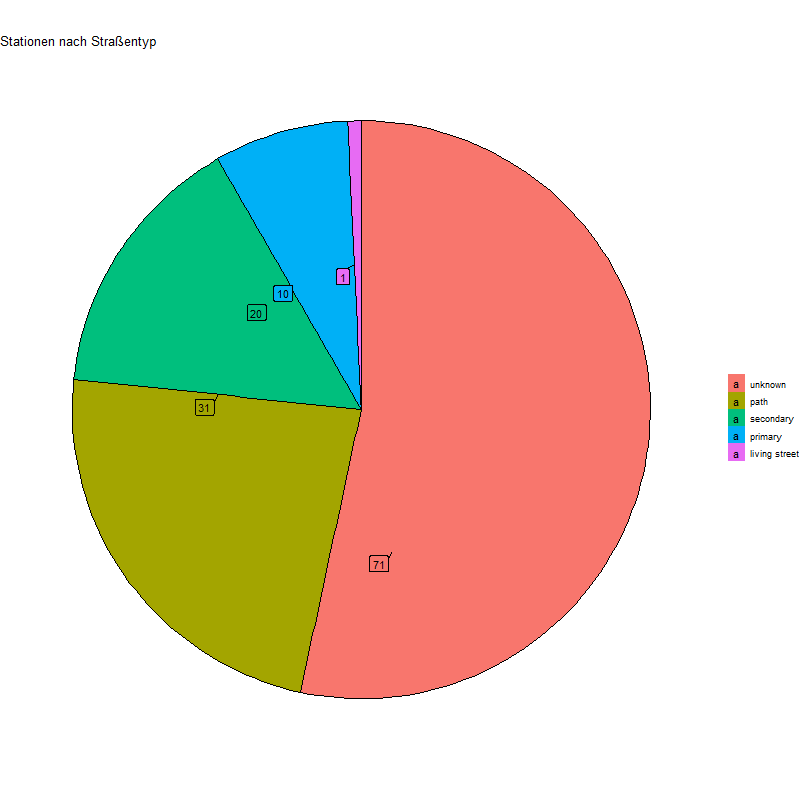
\includegraphics[width=6cm]{Plots/plot20.png} }}%
	\qquad
	\subfloat[\centering neue Aufstellung]{{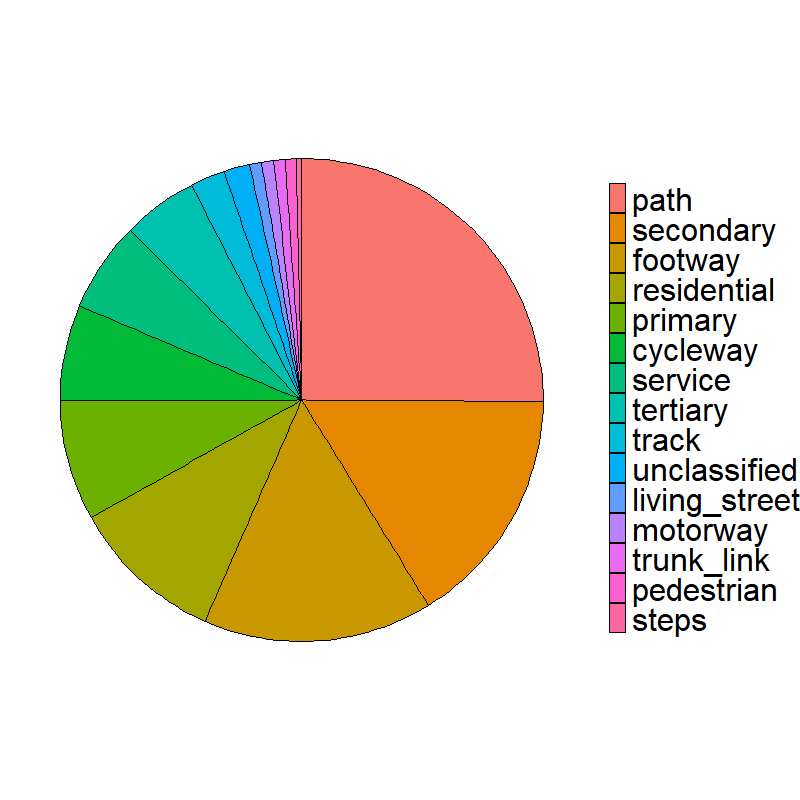
\includegraphics[width=6cm]{Plots/plot52.png} }}%
	\caption{Verteilung von Straßentypen im Datensatz nach der alten Ermittlung}
	\label{Straßentypen}%
\end{figure}

Dazu muss die jeweils kürzeste Entfernung zwischen einem Punkt und einer Linie berechnet werden. Dies funktioniert mithilfe der \lstinline|st_distance| Funktion. Diese Funktion benutzt die Liste aller Koordinaten aller Straßenabschnitte des jeweiligen Straßentyps \lstinline|DT3cycleways| und der Koordinate der Zählstation \lstinline|DT2$geometry|, um daraus die Entfernung eines jedes Straßenabschnitts zum Punkt der Zählstation zu berechnen. Davon ist allein das Minimum interessant. Ist das Minimum geringer als 5 Meter, ist klar, dass die Zählstation nahe des jeweiligen Straßentyps liegt.\\

Im zweiten Datensatz, der erstmals auch Corona Daten inkludierte, wurde dieses Problem anders gelöst, dargestellt in der Abbildung \ref{Straßencheck}. In einem For Loop wurden alle Zählstationen betrachtet. Dabei wurden alle Straßen, die ein kleines Viereck (in der Abbildung \ref{Straßencheck} rot) um die Zählstation (blauer Punkt) herum berührten betrachtet. Die Zählstation wurde jeweils der nächstliegenden Straße (blaue Linie) zu geordnet. Das in der Abbildung gewählte Beispiel stammte von einer Zählstation in Hamburg. Auf diese Weise können aber nicht nur Daten zum Straßentyp festgestellt werden, sondern auch zur Straßenlänge, zum Straßenbelag, zur geltenden Höchstgeschwindigkeit und die Anzahl der Straßenspuren.\\

Genauer beschrieben wird auch wie in \ref{code:street_variables} zu sehen in jedem Loop Durchgang der Datensatz gefiltert nach Zählstationen und die Beobachtungen einer Station landen im Dataframe \lstinline|d|. Für jede Station muss das rote Rechteck wie in der Abbildung \ref{Straßencheck} berechnet werden. Dies geschieht wie in \ref{code:street_variables} mittels der Variable \lstinline|radius| und den Koordinaten aus \lstinline|d|, also den Koordinaten der jeweiligen Zählstation. Die Koordinaten des Vierecks sind so in \lstinline|myLocation| gespeichert.

\begin{lstlisting}[caption={Berechnung der Straßenvariablen},label=code:street_variables]
d=BikeData[BikeData$Station %in% 
	toString(levels(as.factor(
	BikeData$Station))[i]),]

radius = 0.0012
myLocation <- c(d$Lon[1]-radius,d$Lat[1]-radius/1.8,   
	d$Lon[1]+radius,d$Lat[1]+radius/1.8)
\end{lstlisting}

\begin{figure}[!ht]
	\centering
	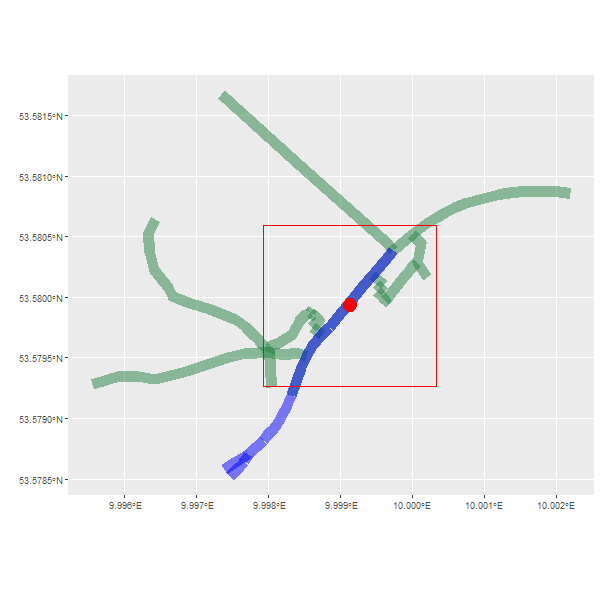
\includegraphics[width=\textwidth]{Plots/Station_5564_1.png}
	\caption{Beispiel der Straßentypanalyse}
	\label{Straßencheck}
\end{figure}

Mit diesen Koordinaten kann nun eine Abfrage von Open Street Map Daten zu der Klasse "highway" gestellt werden. Wie eine solche Abfrage gestellt wird, ist auch im Code \ref{code:osmdata_query} zu sehen. Darauf hin muss die Zählstation der nächstegelegnsten Straße zugeordnet werden. Dies passiert im Code \ref{code:street_variables2}. Dieser besteht aus zwei kürzeren For Schleifen. Die erste wandelt alle Koordinaten der Straßen in ein passendes GPS Format um und ermittelt die jeweils kürzeste Distanz der Straße zu den Koordinaten der Zählstation gespeichert in \lstinline|count_point$geometry|. Für den Fall, dass mehrere Straßen auf der selben Position liegen, ermittelt die Funktion \lstinline|which(dist==mind(dist))| welche dieser Straßen dies sind und wählt von diesen dann diejenige aus, bei der ein Straßenname angegeben ist.

\begin{lstlisting}[caption={Zuordnung zur nächsten Straße},label=code:street_variables2]
j=1
for(j in 1:nrow(streets$osm_lines)){
	street_Points = st_transform(
		streets$osm_lines$geometry[j],4269)
	dist[j] = min(st_distance(
		count_point$geometry, street_Points))
}
	
for(j in which(dist==min(dist))){
	if(length(streets$osm_lines$name[j])>0){
		if(!is.na(streets$osm_lines$name[j])){
			nearest=j
		}
	}
}
\end{lstlisting}

Die Variable \lstinline|nearest| gibt nun an, welche Straße die nächstgelegenste zur Zählstation ist und mit diesen Informationen lassen sich die weiteren notwendigen Variablen berechnen, wie auch in Code \ref{code:street_variables3} beschrieben wird. Wie sich die Straßentypen unter der Anzahl der Zählstationen verteilen, zeigt die Abbildung \ref{Straßentypen} links. Weiter zeigt die Abbildung \ref{VerkehrnachTypen} die Aufteilung des Radverkehrsaufkommens nach der jeweiligen Straßenbeschaffenheit nach Straßenbelag und Straßentyp, wobei die Beschreibungen dem englischen Original der Open Street Map Beschreibung entspricht, denen teils spezifische Definitionen zu Grunde liegen.

\begin{lstlisting}[caption={Berechnung der Straßenvariablen},label=code:street_variables3]
street_type = streets$osm_lines$highway[nearest]
surface = streets$osm_lines$surface[nearest]
lanes = streets$osm_lines$lanes[nearest]
maxspeed = streets$osm_lines$maxspeed[nearest]
streetlengths = st_length(street_Points[nearest])
\end{lstlisting}


\begin{figure}[!ht]%
	\centering
	\subfloat[\centering nach Straßentypen]{{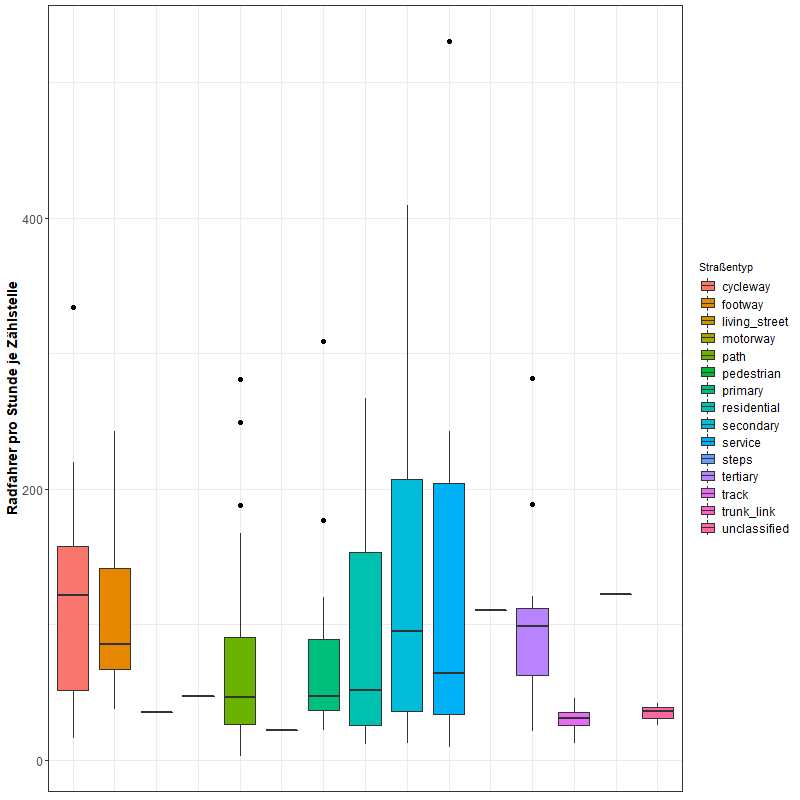
\includegraphics[width=6cm]{Plots/plot60.png} }}%
	\qquad
	\subfloat[\centering nach Straßenbelag]{{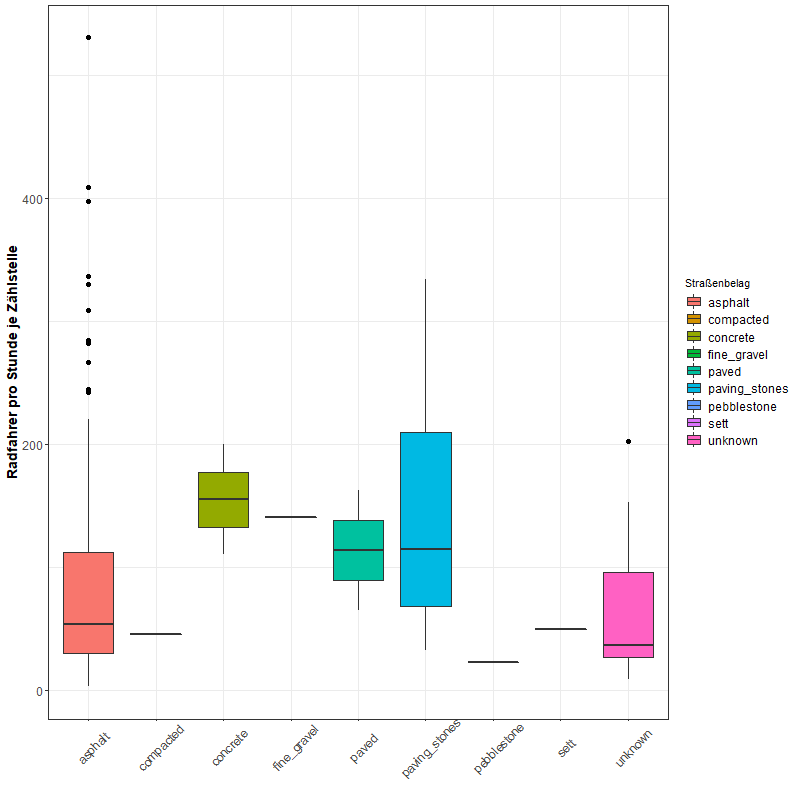
\includegraphics[width=6cm]{Plots/plot61.png} }}%
	\caption{Radverkehr nach Straßenbeschaffenheit}
	\label{VerkehrnachTypen}%
\end{figure}

\subsection{Sonstige}

Weitere wichtige Variablen sind Feier und Ferientage. Dazu wurde eine Liste dieser Tage händisch für alle Bundesländer angelegt und diese automatisch in den Datensatz übertragen. Informationen zu den Ferien- und Feiertagen seit 2012 nach den jeweiligen Bundesländern stammen von der Seite \url{www.kalenderpedia.de}.

\chapter{Verwendete Methoden}

Das vorangegangene Kapitel gab einen genauen Überblick über die bestehende Literatur, die sich mit der Vorhersage des Aufkommens von Fahrrädern in urbanen Zentren beschäftigt. Immer häufiger wurden dabei Machine Learning Methoden zur Schätzung eines Modells verwendet. Um die Übersichtlichkeit der Arbeit zu gewährleisten, wurden Erläuterungen, über die verschiedenen verwendeten Methoden, bis zu diesem Zeitpunkt aufgespart, um einen gegliederten Überblick zu ermöglichen.\\
Im Folgendem wird die Funktionsweise von Regressionssystemen, Support Vector Systemen, Entscheidungsbaum Varianten und neuronalen Netzwerken erklärt. Die Auswahl dieser Schwerpunkte beruht auf der Verwendung in der bisher dargestellten Literatur. Hat man ein geeignetes Modell ausgewählt, lässt sich dessen Effizienz mit dem richtigen Validierungsverfahren noch weiter steigern. Deswegen beinhaltet dieses Kapitell ebenfalls eine kurze Erläuterung der Cross Validation.

\section{Problem zur Autokorrelation}

Vorab muss das Problem der Autokorrelation erwähnt werden. Autokorrelation bezeichnet wie der Name fast sagt, die Korrelation innerhalb einer Variable und nicht wie sonst die Korrelation zweier verschiedener Variablen. Diese Autokorrelation kann räumlich und zeitlich auftreten. Bei der zeitlichen Autokorrelation ähneln sich Werte, die zeitlich nah bei einander liegen. Bei der räumlichen Autokorrelation ähneln sich Werte, die räumlich nah bei einander liegen.\\ 
Dies kann zu Problemen führen. So beschreiben \cite{LiuAutocorrelation2022}, dass räumliche Autokorrelation die Annahme von unabhängig und identisch verteilte Zufallsvariablen verletzt. Dies kann zu Overfitting oder einem Bias der Vorhersagen führen. Im Fall von OLS Regressionen ist der Standardfehler nicht mehr konsistent, was Aussagen über die Signifikanz des Modells wertlos macht. So beschreibt es auch Stock and Watson \cite{Stock2015b}. Da das Ziel dieser Masterarbeit jedoch nur die Vorhersage ist, ist die Signifikanz nicht entscheiden. Um gute Vorhersagen zu treffen, ist es jedoch notwendig, das Risiko von Overfitting oder einer Verzerrung zu minimieren. Dazu gibt es drei Lösungsansätze. Diese wären die Verwendung von Lagged Variablen, Feature Engienering und Resampling.\\

\subsection{Lagged Variablen}

Der Begriff Lagged Variable bezeichnet die Aufnahme einer versetzten Beobachtung, die als zusätzliche Variable mit in das Modell aufgenommen wird. Im Bereich von Zeitreihendaten wird also eine zeitlich vorhergehende Beobachtung der eigentlich abhängigen Variable in das Modell aufgenommen. Im Fall der Regression nennt man ein solches Vorgehen Autoregression. Dies beschreiben z.B. \cite{Stock2015a}. Die mathematische Formulierung einer allgemeinen Autoregression lautet:

\begin{equation}
	\label{SVM:Autoregression}
	y_t = \beta_0 + \beta_1 * y_{t-1} + \beta_2 * y_{t-2} + ... + \beta_p * y_{t-p} + u_t
\end{equation}

Diese Formulierung kann natürlich nicht nur in OLS Regressionen angewendet werden, sondern auch bei allen weiteren Machine Learning Algorithmen, über die hier noch beschrieben werden. Eine weiter Entwicklung dieses Ansatz ist die ARIMA-Modellierung, was die Abkürzung für Auto Regressive-Moving Average ist.\\
Problem an diesem Ansatz ist, dass er für die Vorhersage an unbekannten out of sample Orten nicht anwendbar ist, weil an unbekannten Orten auch vorhergehende Beobachtungen unbekannt sind, die man in das Modell zur Vorhersage mit aufnehmen müsste. Deswegen ist die Aufnahme von Lagged Variablen nicht geeignet für diese Masterarbeit.

\subsection{Erklärende Variablen}

Eine weitere Möglichkeit Autokorrelation zu vermeiden ist es, Variablen in das Modell aufzunehmen, die die Autokorrelation erklären können. Nimmt man in einem zeitlichen Modell z.B. die Stunden als Variable auf, die erklären können, dass in der Mittagszeit viele Fahrradfahrer auf den Straßen sind und Nachts nur sehr wenige, dann erklärt das auch, warum zu zwei Zeitpunkten, die nah beieinander z.B. um die Mittagszeit herum, ähnlich hohe Werte aufzeigen. Dies funktioniert ähnlich auch für räumliche Autokorrelation. Nimmt man als Variable die Entfernung zum Stadtzentrum auf, dann erklärt dies nicht nur, dass nahe des Stadtzentrums viele Radfahrer unterwegs sind und dafür weniger Radfahrer außerhalb des Stadtzentrums, es ekrlärt auch, wieso sich zwei nahe beieinander liegende Punkte ähneln, weil beide weit weg vom Stadtzentrum liegen.\\
Diesen Ansatz verfolgt auch die Studie von \cite{LiuAutocorrelation2022}, automatisiert jedoch diesen Prozess. Sie schlagen für Random Forest z.B. vor, Probleme mit Autokorrelation zu vermeiden, in dem gewichtete räumliche Variablen durch das LASSO Regressionsverfahren selektiert werden. Diese räumliche Variablen übernehmen die vorher besprochene Rolle. Die LASSO Regression ist neben der RIDGE Regression eines von zwei Regularisierungsverfahren. Dabei wird eine Regression aufgesetzt, in deren Optimierungsproblem nicht nur die quadrierte Summe der Fehlerterme steht, sondern dazu addiert die quadrierte (RIDGE) oder absolute (LASSO) Summe der Estimatoren selbst. Ziel einer solchen Optimierung ist es, die Estimatoren zu schrumpfen, wobei bei LASSO sogar Estimatoren auf null setzen kann und somit Feature Selection betreiben kann.\\
Ein solches Modell aufzusetzen, übersteigt jedoch den Arbeitsumfang dieser Arbeit. Was die zeitliche Autokorrelation angeht, können die Variablen zur Stunde und zum jeweiligen Monat Auschluss geben. Was die räumliche Autokorrelation angeht, stehen so viele Variablen zur Auswahl, dass es hier durchaus Sinn machen könnte, eine genauere Feature Selektion zu betreiben. Ein solches Verfahren jedoch erfordert leistungsfähigere Hardware, würde aber gleichzeitig die Performance des Modells nicht drastisch erhöhen.

\subsection{Resampling}

Resampling bezeichnet eine Neuanordnung von Beobachtung eines Datensatzes, sodass dabei ein neuer Datensatz entsteht. Beispiele hierfür ist das Bootstraping, bei dem eine Mehrfachziehung zufällig ausgewählter Beobachtungen erlaubt ist. Daneben ist Resampling auch ohne Mehrfachziehung von Beobachtungen nötig. Diese führt dazu, dass man weniger Beobachtungsdaten zieht, als im Datensatz vorhanden sind. Dabei handelt es sich um Undersampling.\\
Undersampling kann auch dabei helfen, Autokorrelation zu vermeiden, denn verringert man die Dichte an Beobachtungen, spielt die zeitliche oder räumliche Nähe einzelner Beobachtungen zu einander einer geringere Rolle. Der große Nachteil dieser Methode, ist dass durch ein Verzicht dieser Daten auch Informationen verloren gehen und das Modell durch die kleinere Sample Size eine schlechtere Performance vorweißt. Im Fall dieser Arbeit steht ein Datensatz zur Verfügung, der mehr als groß genung ist, um Undersampling zuzulassen. Zudem kommt hinzu, dass der der technische Flaschenhals im Arbeitsspeicher es notwendig machen wird, die Sample Size des Datensatzes zu verkleinern.

\section{OLS Regression}

Einer der einfachsten und geläufigsten Methoden ist die Regressionsanalyse. So nutzen \cite{Holmgren2017}, \cite{Alattar2021} und \cite{Gao2022} z.B. ein lineares Regressionssystem und \cite{Wessel2020} ein log-lineares sowie ein negativ binomiales Regressionssystem.\\
Das Prinzip einer einfachen OLS (Ordinary Least Square) Regression besteht darin, den Zusammenhang zwischen zwei Variablen zu finden, der die Summe der quadrierten Fehlerterme, also die Abweichung tatsächlicher Beobachtungen zur Regressionsgerade, minimiert. Als Maß zur Validierung eines solchen Modells ließe sich z.B. das Bestimmtheitsmaß R$^2$ nutzen, also der Anteil der Streuung, der durch die Regression erklärt werden kann, aber auch z.B. die Wurzel der summierten quadratischen Fehler (RMSE). Ein solches Fehlermaß oder Bestimmtheitsmaß, dass die Performance des Modells bewertet ist nützlich, einen Vergleich zu ziehen, verwendet man mehrere Modelle, wie es zB \cite{Holmgren2017}, \cite{Broucke2019} oder \cite{Gao2022} machen.

\section{Support Vector Regression}


In der bisher betrachteten Literatur haben \cite{Holmgren2017}, \cite{Broucke2019}, \cite{Xu2013} und \cite{Gao2022} Support Vector Machines bzw Support Vector Regressionen verwendet. \cite{Pisner2020} schildern Support Vector Machines als eine supervised Calssification Methode, die eine Hyperebene nutzt, um Daten nach unterschiedlichen Ausprägungsmustern zu trennen und so den jeweiligen Klassen zu zuordnen. Diese Vorgehensweise ist auch dargestellt in Abbildung \ref{SVM}. Nun könnte diese Trennlinie, auch Hyperplane genannt, so gewählt werden, dass sie das Margin, also den Abstand zwischen der Trennlinie selbst und der nächstgelegenen Beobachtung, maximiert. Dieses Vorgehen wird auch als Maximum Margin Classification bezeichnet. Jedoch falls innerhalb des maximalen Margin-Bereichs eine neue zufällige Beobachtung hinzu kommt, dann führt diese zu einer starken Veränderung der Trennlinie selbst. Ausreißer Daten können so zu einer starken Verzerrung führen und eine Generalisierbarkeit wäre nicht gegeben.
\begin{figure}[!ht]
	\centering
	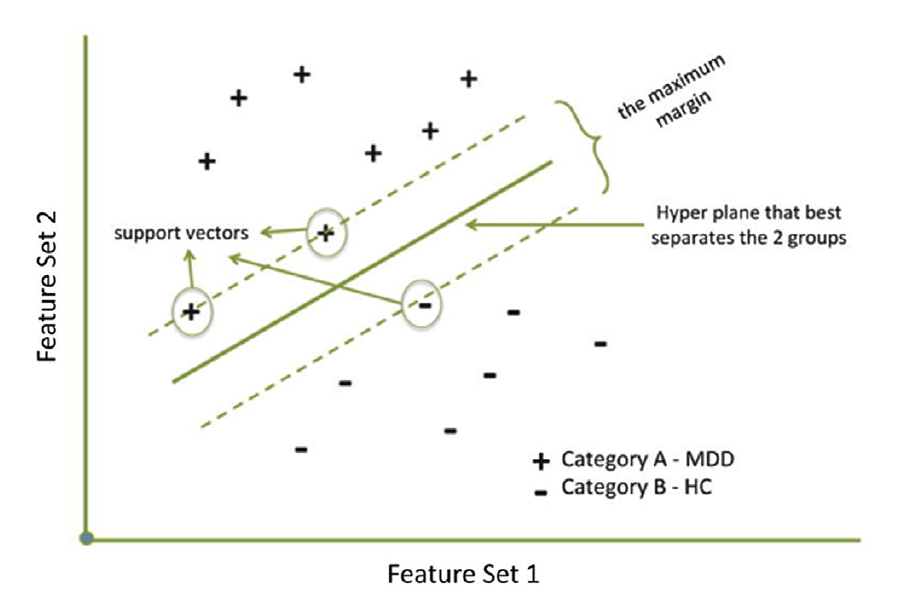
\includegraphics[width=\textwidth]{Plots/SVM.png}
	\captionsource{Hyperebenen (Hyperplanes) in Support Vector Machines}{
		\cite{Pisner2020}
	}
	\label{SVM}
\end{figure}\\
Deswegen nutzt man oft soft Margins, die die Missklassifikation von Ausreißern zu lassen. Dabei stellt $\xi$ die Variable für die Toleranz von Missklassifikationen dar, auch oft Slack Variable genannt. Ist $\xi=0$ so erhalten wir ein hard Margin Classifier.
\begin{figure}[!ht]
	\centering
	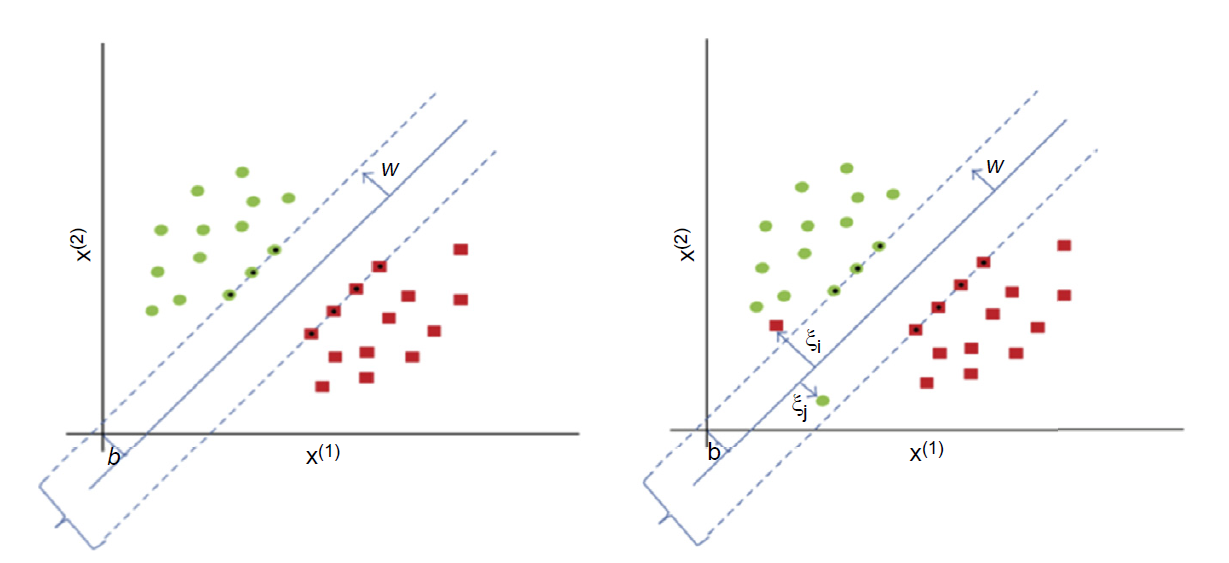
\includegraphics[width=\textwidth]{Plots/SVM2.png}
	\captionsource{Soft Margins in Support Vector Machines}{
		\cite{Pisner2020}
	}
	\label{SVM2}
\end{figure}\\
Mathematisch formulieren \cite{James2013SVM} eine Hyperplane in einem p-dimensionalen Raum wie folgt:
\begin{equation}
	\label{SVM:Hyperplane}
	\beta_0 + \beta_1 X_1 + \beta_2 X_2 + ... + \beta_p X_p = 0
\end{equation}
Dabei liegt der Normalenvektor $\beta=(\beta_1, \beta_2, ..., \beta_p)$ in der orthogonalen Richtung zur Hyperplane. Das Optimierungsproblem hinter der soft Margin ($M$) Klassifikation sieht wie folgt aus:
\begin{equation}
	\label{SVM:SoftMarginClassifier}
	\begin{aligned}
		&\underset{\beta_0, \beta_1, ... , \beta_p,M,\xi_1,...,\xi_n}{\text{max}}M \\
		&\text{udN}\: \sum_{j=0}^p\beta_j^2=1, \\
		&y_i(\beta_0 + \beta_1 x_{i1} + ... + \beta_{ip}) \geq M(1-\xi_i),\\
		&\xi_i \geq 0, \sum_{i=0}^n\xi_i \leq D,
	\end{aligned} 
\end{equation}
Hier taucht nun die Slack Variable auf, die einen Toleranzbereich für Missklassifikation ermöglicht. Setzt man $\xi=0$, erhält man einen hard Margin Classifier. D ist ein nichtlinearer Tuning Parameter. Natürlich kann man in der Funktion des Hyperplanes (\ref{SVM:Hyperplane}) Polynomiale aufnehmen und so einen nicht linearen Classifier erhalten.\\
Grundlegendes Problem ist nun, dass in der Vorhersage des innerstädtischen Fahrradaufkommens kein Klassifikationsproblem besteht, so wie es eine Support Vector Machine lösen würde. Deswegen bietet es sich an, eine Support Vector Regression zu nutzen, so wie es z.B. \cite{Holmgren2017} macht. Während herkömmliche OLS Regression die summierten quadratischen Fehlerterme minimiert, minimiert Support Vector Regression, so beschreiben es \cite{Awad2015}, eine Loss Function, die Fehlvorhersagen bestraft. Dieser Vorgang ist auch eine Verallgemeinerung des bisher beschriebenen Klassifikations Algorithmus.\\ 
\begin{figure}[!ht]
	\centering
	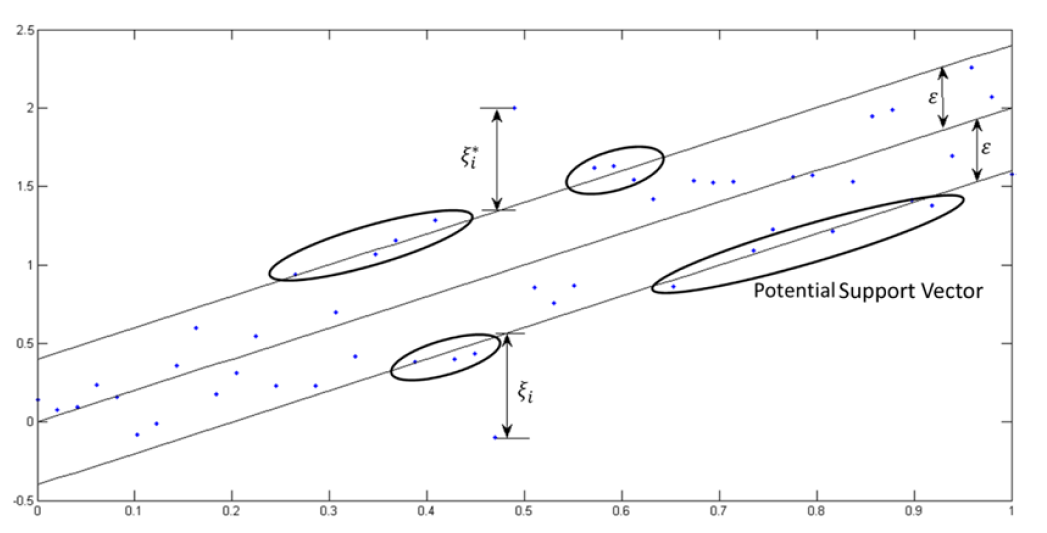
\includegraphics[width=\textwidth]{Plots/SVM3.png}
	\captionsource{Eindimensionale lineare SVR}{
		\cite{Awad2015}
	}
	\label{SVM3}
\end{figure}\\
Wo im Soft Margin Classifier $\xi$ genutzt worden ist, um auch Missklassifikationen zuzulassen, wird nun ein unempfindlicher Bereich von $\varepsilon$ um die Hyperplane herum gelegt, sodass ein Großteil der Beobachtungen im eigentlichen Margin Bereich zu finden sind. Aus der Hyperplane, die eigentlich Beobachtungen trennen soll wird so die regressive $\varepsilon$-Tube, eine wertbeständige Funktion. Dargestellt ist dies auch in der Abbildung \ref{SVM3}.\\
Die Slack Variable $\xi$ wird so zur Toleranz Variable für Ausreißer von der $\varepsilon$-Tube und so zum Bestandteil der Loss Function, die man versucht zu minimieren. Zusammen mit C der Gewichtung der Minimierung ergibt das:
\begin{equation}
	\label{SVM:Regression}
	\begin{aligned}
		&\underset{\beta_0, \beta_1, ... , \beta_p,M,\xi_1,...,\xi_n}{\text{min}}\frac{1}{2}||\beta||^2 + C\sum_{i=1}^N \xi_i + \xi_i^*\\
		&\text{udN}\; y_i - \beta^T x_i \leq \varepsilon + \xi_i^*, \; i=1...N\\
		&\beta^T x_i - y_i \leq \varepsilon + \xi_i^, \; i=1...N\\
		&\xi_i, \xi_i^* \geq 0, \; i=1...N
	\end{aligned} 
\end{equation}
Der Vorteil dieser Vorgehensweise ist, dass man durch den Optimierungsprozess ein Modell erhält, das sehr robust auf Ausreißer reagiert trotzt hoher Präzession durch die Nutzung von $\xi$.

\section{Random Forests Regression}

Entscheidungsbaum Methoden finden sich bei \cite{Holmgren2017}, \cite{Broucke2019}, \cite{Mitchell2018PredictingBT} und \cite{Gao2022}. Dabei sind diese simpel, nicht immer aber besonders präzise so \cite{James2013TBM}. Es sei denn man nutzt komplexere Weiterentwicklungen wie Random Forests. Diese nutzen auch \cite{Holmgren2017}, \cite{Broucke2019} und \cite{Mitchell2018PredictingBT}.\\ 
Ein Vorteil für diese Hausarbeit ist weiter, dass Entscheidungsbaum Methoden sowohl zur Klassifikation, als auch zur Regression genutzt werden können so \cite{James2013TBM}. Die Begrifflichkeit rührt von der Struktur in der Entscheidungsbäume Daten aufbereiten, denn ihre Darstellungsweise erinnert an eine umgedrehte Baumkrone, in der jede Astgabelungen ein Statement darstellt, welches mit wahr oder falsch beantwortet werden kann. Die Beobachtungen aus dem Datensatz folgen entlang ihrer Ausprägung verschiedenen Astgabelungen und werden so einer Vorhersage zugeordnet. Dies kann z.B. aussehen, wie in Abbildung \ref{DTM1}.
\begin{figure}[!ht]
	\centering
	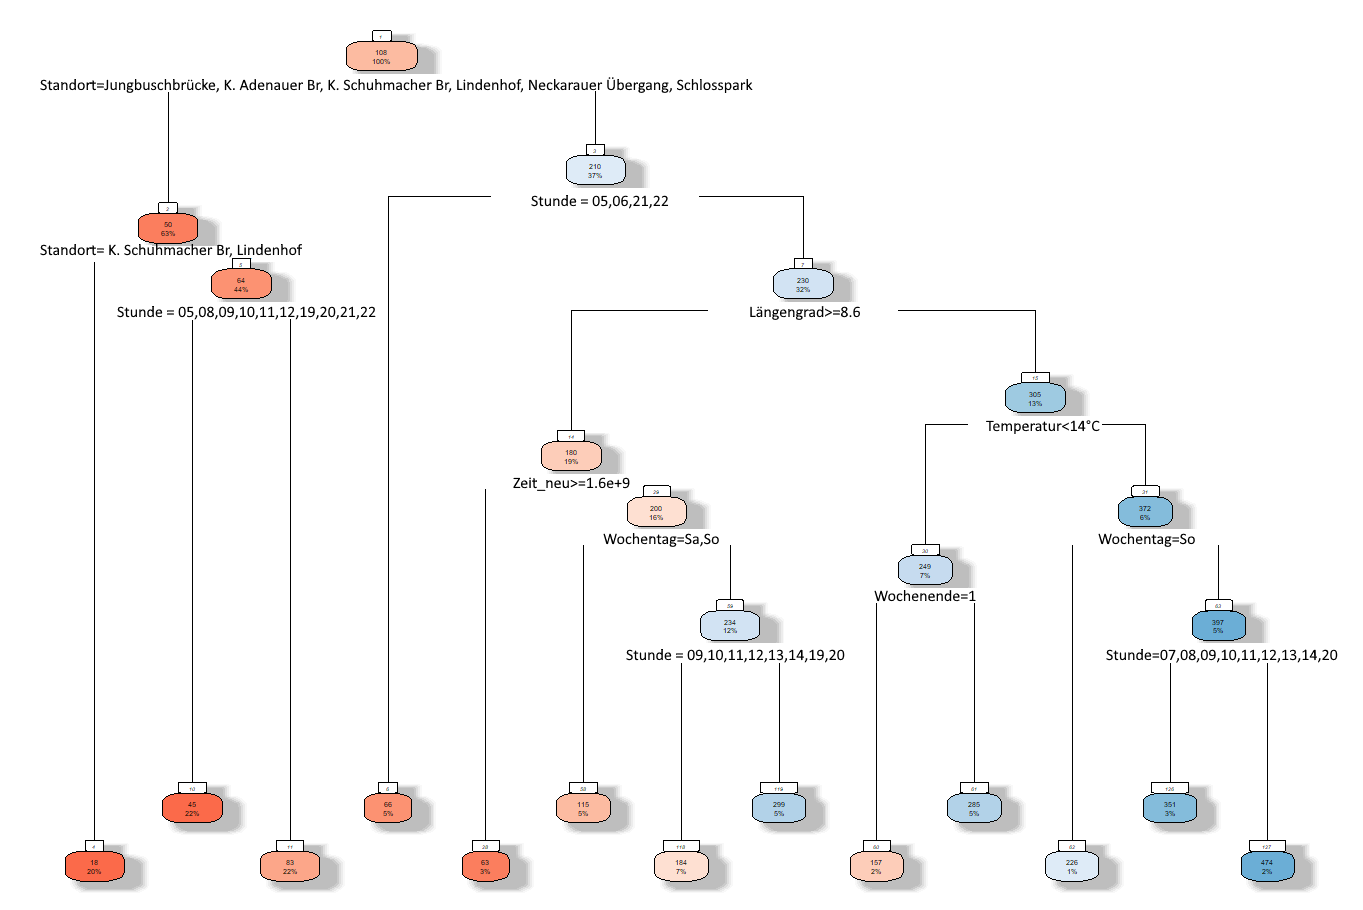
\includegraphics[width=16cm]{Plots/Entscheidungsbaum.png}
	\captionsource{Ein Entscheidungsbaum basierend auf Daten von Fahrradzählstationen in Mannheim und Daten des DWD 2016 bis 2022.}{
		Eigene Darstellung
	}
	\label{DTM1}
\end{figure}\\
Durch diese Entscheidungsgrenzen unterteilt der Entscheidungsbaum den Prädiaktorenraum in distinkte sich nicht überlappende Regionen $R_1,R_2,...,R_J$. Das Optimierungsproblem besteht nun darin, $R_1,R_2,...,R_J$ so zu wählen, dass die Summe der quadrierten Residuen (RSS) minimiert wird: 
\begin{equation}
	\label{TDM:TreeOptimization}
	\sum_{j=1}^J\sum_{i\in R_j}(y_i - \hat{y}_{R_j})^2
\end{equation}
Auf diese Weise lässt sich ein Entscheidungsbaum erstellen. Bei den zuvor angesprochenen Random Forests wird diese Vorgehensweise mit einem Bootstraps Verfahren kombiniert. Bootstraping bedeutet, dass durch zufällige Ziehungen von Beobachtungen aus einem bestehenden Datensatz, wobei mehrfach Ziehungen erlaubt sind, ein neuer Bootstraps Datensatz erstellt wird, der dem ursprünglichen Datensatz ähnelt, jedoch davon abweicht. Diese Praxis führt man mehrere male durch und wendet auf jeden Bootstraps Datensatz einen Entscheidungsbaum an, so das man eine große Anzahl von Entscheidungsbäumen erhält. Möchte man nun auf neuen Beobachtungen eine Vorhersage treffen, lässt man diese durch die Bootstraps Entscheidungsbäume laufen, wobei man sich auf die Vorhersage festlegt, die am meisten von den Bootstraps Entscheidungsbäumen bestimmt wurde. Dieses Verfahren führt zu einer deutlichen Steigerung der Vorhersage Genauigkeit.

\section{Neuronale Netze}


Deep Learning Algorithmen und die dazu gehörigen neuronalen Netzwerke sind mit die fortgeschrittenste Form im Bereich des Machine Learnings. Sie tauchen bei \cite{Broucke2019} und \cite{Mitchell2018PredictingBT} auf.
\subsection{Aufbau eines neuronalen Netzes}
Zur Verdeutlichung der Funktionsweise von neuronalen Netzwerken beschränkt sich diese Arbeit aufgrund von Übersichtlichkeit auf Single Layer Perceptrons, diese sind die einfachste Form eines neuronalen Netzes und bestehen nur aus einer Schicht von Neuronen. Eine graphische Darstellung eines solchen Netzwerkes ist in Abbildung \ref{NN1} zu sehen.
\begin{figure}[!ht]
	\centering
	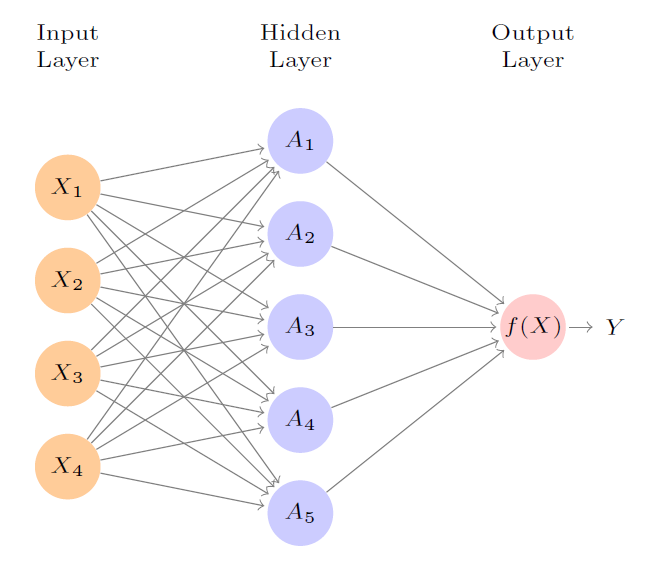
\includegraphics[width=12cm]{Plots/NN1.png}
	\captionsource{Neural network with a single hidden layer}{
		\cite{James2013DL}
	}
	\label{NN1}
\end{figure}\\
Mathematisch ausgedrückt, gleicht dieses Netzwerk einer Vektor Multiplikation. Im Input Vektor (Input Layer), sind die Variablen einer jeden einzelnen Beobachtungen zu finden. Diese werden mit Gewichten im Hidden Layer multipliziert. Wobei jeder einzelner Punkt in diesem Layer, auch Neuron genannt, über ein separates Gewicht verfügt. Diese sind so eingestellt, dass im Output eine möglichst zielgenaue Vorhersage zustande kommt. Als Formel sieht diese Vorgehensweise wie folgt aus:
\begin{equation}
	\label{NN:SingleLayerNetwork}
	\begin{aligned}
		f(x)& = \beta_0 + \sum_{k = 1}^K \beta_k h_k (X)\\
		& = \beta_0  + \sum_{k = 1}^K \beta_k \underbrace{ g(w_{k0} + \sum_{j = 1}^p w_{kj} X_)}_{\text{Aktivierungsfunktion}}
	\end{aligned} 
\end{equation}
Ob und in welchem Umfang die Information, die ein Neuron passiert, weiter gereicht wird, entscheidet die Aktivierungsfunktion $g(z)$. In ihr werden die Informationen des Inputs und die der Gewichte übertragen. Das kann z.B. durch eine Sigmoid Funktion (\ref{NN:Sigmoid}) oder durch eine ReLU (Rectified Linear Unit) Funktion (\ref{NN:ReLU}) geschehen.
\begin{equation}
	\label{NN:Sigmoid}
	g(z)=\frac{e^z}{1+e^z}=\frac{1}{1+e^{-z}}
\end{equation}
\begin{equation}
	\label{NN:ReLU}
	g(z)=\begin{cases}
		0 \; \text{wenn $z<0$}
		\\
		z \; \text{sonst}.
	\end{cases}
\end{equation}
\begin{figure}[!ht]
	\centering
	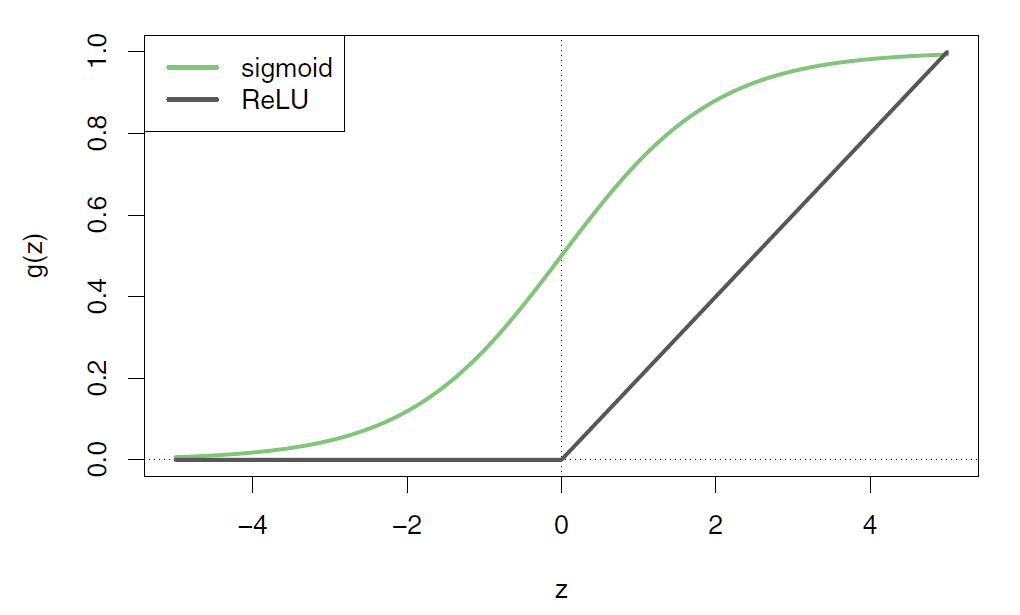
\includegraphics[width=10cm]{Plots/NN2.png}
	\captionsource{Aktivierungsfunktionen}{
		\cite{James2013DL}
	}
	\label{NN2}
\end{figure}\\
Die Sigmoid Funktion wird z.B. auch für die logistische Regression genutzt. Der Vorteil der ReLU Funktion besteht darin, dass Neuronen ausgeschaltet werden, sollte $z$ zu klein sein, wodurch Rechenkraft gespart wird. Zu dem reagiert das Neuronale Netz stärker auf höhere Werte von $z$ und lernt damit schneller.
\subsection{Berechnung eines neuronalen Netzes}
Wichtig damit die Aktivierung eines Neurons zur richtigen Vorhersage führt, ist das richtig trainierte Gewicht $w_{kj}$. Sowohl die Parameter $\beta_0, ..., \beta_K$ als auch $w_{10}, ..., w_{Kp}$ müssen trainiert werden. Das Optimierungsproblem dazu besteht in:
\begin{equation}
	\label{NN:Optimization}
	\underset{ \{ w_k \}^K_1 , \beta }{\text{min}}\frac{1}{2}\sum_{i=1}^n (y_i-f(x))^2
\end{equation}
Um diese Optimierung vorzunehmen verwendet man den Vektor $\theta$, der alle zu optimierenden Variablen enthält. Der Fehlerterm ergibt dann:
\begin{equation}
	\label{NN:ErrorTerm}
	R(\theta)=\frac{1}{2}\sum_{i=1}^n (y_i-f_{\theta}(x))^2 \; \; \text{mit} \; \theta=(\{ w_k \}^K_1,\beta)
\end{equation}
Zu Beginn des Optimierungsprozesses wird $\theta^{t=0}$ angenommen, dass heißt der Vektor beginnt ungewichtet. Darauf hin folgen Wiederholungen eines Prozesses, bei dem ein Vektor $\delta$ gefunden werden muss, sodass $\theta^{t+1}=\theta^t + \delta$ zu $R(\theta^{t+1})<R(\theta^t)$. In jedem Durchlauf dieses Prozess wird $t$ erhöht. Eine eindimensionale Veranschaulichungen dieses Prozesses ist in Abbildung \ref{NN3} zu finden.
\begin{figure}[!ht]
	\centering
	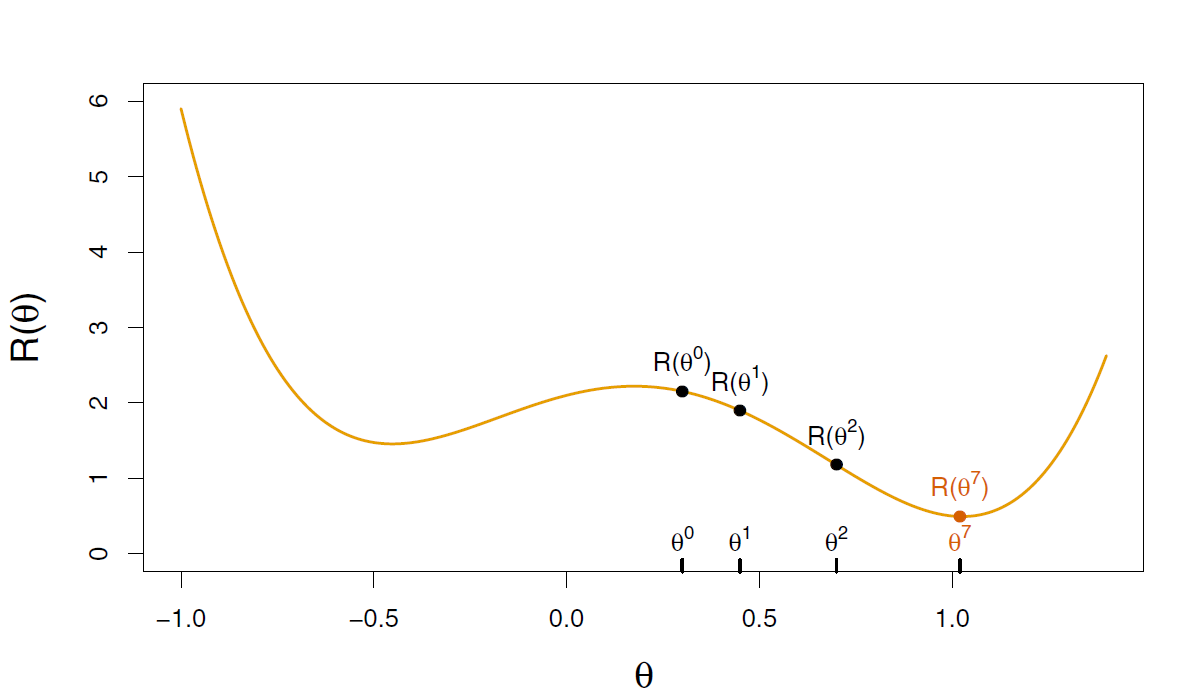
\includegraphics[width=14cm]{Plots/NN3.png}
	\captionsource{Gradiemt Descent}{
		\cite{James2013DL}
	}
	\label{NN3}
\end{figure}\\
Wie kann aber der Vektor $\delta$ gefunden werden, sodass der Fehlerterm gesenkt wird? Dazu muss man den Vektor des Gradienten berechnen:
\begin{equation}
	\label{NN:GradientVector}
	\Delta R(\theta^m)=\frac{\partial R(\theta)}{\partial \theta}|_{\theta=\theta^t}
\end{equation}
Der partielle Vektor der Ableitung der aktuellen Schätzung von $\theta^t$ zeigt aufwärts. Um also $\delta$ zu finden gehen wir in die entgegen gesetzte Richtung gewichtet mit der Lernrate $\rho$. So ergibt sich:
\begin{equation}
	\label{NN:Lernfunktion}
	\theta^{t+m} \leftarrow \theta^m -\rho \Delta R(\theta^m)
\end{equation}
Die Ableitungen des Fehlerterms nach den Gewichten, die wir brauchen, um den Gradientenvektor in \ref{NN:GradientVector} zu bestimmen, kann man durch die Ketten Ableitungsregel vereinfachen:
\begin{equation}
	\label{NN:ChainRule}
	\begin{aligned}
		\frac{\partial R_i(\theta)}{\partial \beta_k}& = \frac{\partial R_i(\theta)}{\partial f_{\theta} (x_i)} \frac{\partial f_{\theta} (x_i)}{\partial \beta_k}\\
		& = -(y_i - f_{\theta})g(z_{ik})\\
		\frac{\partial R_i(\theta)}{\partial w_{kj}}& = \frac{\partial R_i(\theta)}{\partial f_{\theta} (x_i)} \frac{\partial f_{\theta} (x_i)}{\partial g(z_{ik})} \frac{\partial g(z_{ik}) }{\partial z_{ik}} \frac{\partial z_{ik}}{\partial w_{kj}}\\
		& = -(y_i - f_{\theta})\beta_k*g'(z_{ik})x_{ij}\\
		\text{mit}& \; \; z_{ik}=w_{ko}+ \sum^p_{j=1}w_{kj}x_{ij}
	\end{aligned} 
\end{equation}

\section{Validation}

Statistische Modelle wie ein neuronales Netz machen erstaunlich präzise Vorhersagen. Doch wie kann man eine solche Präzession messen? Dafür verantwortlich ist die Validierung. Mittels Maße wie dem Bestimmtheitsmaß R$^2$ oder dem RMSE kann man die Performance der Vorhersagen im Vergleich mit den tatsächlichen Daten messen.\\
Doch wie validiert man die Vorhersagekraft eines Modells auf Daten, mit denen das Modell selbst nicht trainiert worden ist, um zu testen ob das Modell die eigenen Daten nicht overfittet? Hierzu ließe sich der Validation Set Approach nutzen. Teilt man die Beobachtungen in zwei unterschiedlichen Sets zufälligerweise auf, erhält man ein Set, mit dem man ein Modell trainieren kann und eines mit dem man es testen kann. Die Quote nach der man diese Beobachtungen aufteilt nennt man Split. Ein häufig verwendeter Split ist 80 \% für das Trainings Set und 20 \% für das Test Set.

\subsection{Cross Validation}

Eine Weiterführung dieses Konzepts ist die Cross Validation. Hier wird der Datensatz nicht in 2 sondern in $k$ viele und gleichgroße Sets unterteilt. Es werden dann $k$ viele Validierungen vorgenommen. Bei jedem Durchlauf wird eines der Sets zur Validierung und die restlichen Sets zum Training verwendet. Das bietet den Vorteil, dass der gesamte Datensatz zur Validierung und zum Training verwendet wird, während beim herkömmlichen Ansatz immer auf ein Teil der Daten verzichtet werden musste. Außerdem werden so mehr Stichproben erhoben. Man vergleicht nicht ein Modell sonder k-viele Modelle. Es kann immer vorkommen, dass viele Modelle solide performen, während eines der Modelle zeigt, dass es zu drastischen Fehlern kann. Das heißt die Wahrscheinlichkeit Overfitting aufzudecken ist größer.

\subsection{Conditional Validation Set Building}

In dem Fall der Daten der Radzählstation gäbe es zusätzliches Problem, dass auch die Validierung mit dem Validation Set Approach Overfitting wahrscheinlich nicht richtig erkennen ließe. Denn durch eine rein zufällige Aufteilung der Daten in verschiedene Sets, ließe sich die wahre externe Validität des Modells nicht prüfen, denn auch dann träfe das Modell immer vorhersagen für fixe räumliche Punkte, die bereits auch im Trainings Datensatz vorkamen.\\
Um dieses Problem zu umgehen, muss man die Aufteilung der Daten in die verschiedenen Sets auf die Ausprägung der Stationen kondititionieren. Das heißt jede Zählstation darf in jedem Set nur einmal vorkommen, damit im Test Set immer Orte vorhanden sind, die dem Modell unbekannt sind. Diese Aufgabe übernimmt der folgende Code:

\begin{lstlisting}[caption={Aufteilung der Zählstationen},label=code:valSetBui]
while(length(stations_not_chosen)>0)
{
	x1 <- sample(1:length(stations_not_chosen), 1)
	newStation = stations_not_chosen[x1]
	
	stations_splits[stations_splits$Station == 
		newStation,]$Split = actual_split
	
	observations_per_splits$
		Observations[actual_split] = 				
		observations_per_splits$
		Observations[actual_split] + 
		Obs_perStation[Obs_perStation$Station== 
		newStation,]$Observations
	
	stations_not_chosen = stations_not_chosen[-x1]
	
	if(median(observations_per_splits$Observations)
	<=observations_per_splits$
	Observations[actual_split]){
		
		actual_split = actual_split + 1
		if(actual_split>validation_splits)
		{actual_split=1}
		
	}
}
\end{lstlisting}

In dem Code \ref{code:valSetBui} werden innerhalb einer \lstinline|while()| Schleife alle Stationen einem der k-vielen Sets hinzugefügt, bis die Schleife die Anzahl der zu verordnenden Zählstationen in \lstinline|stations_not_chosen| herunter gezählt hat. Die Anzahl von k ist 5 und ist in der Variable \lstinline|validation_splits| gespeichert. Damit alle Validierungssets ungefähr gleich viele Beobachtungen haben, zählt der Code \ref{code:valSetBui} mit, wie viele Beobachtungen mit jeder Station einem Set hinzugefügt werden. Diese Anzahl wurde zuvor in der Tabelle \lstinline|Obs_perStation| gespeichert. Ob im folgendem Durchlauf der \lstinline|while()| Schleife das nächste Validierungsset ausgewählt wird, oder nochmal dasselbe hängt an der Anzahl der Beobachtungen. Jedes Validierungsset wird solange mit Zählstationen befühlt, bis der Median an Beobachtungen aller Sets gleich ist oder überschritten wurde. Dies wird in der \lstinline|if()| Schleife abgefragt.\\
Auf diese Weise erhält man fast gleichgroße unterschiedliche Validierungsset, in denen jede Zählstation nur einmal vergeben ist. Teilweise kommt es auch vor, dass ganze Städte nur in je einem Validierungsset vertreten sind, weil es Städte gibt, die nur eine Zählstation mit sich bringen.

\subsection{Weighted Subset Building}

Im Verlauf dieser Masterarbeit sind einige Probleme durch die Größe des Datensatzes entstanden. Da der Datensatz über vier Millionen Beobachtungen beinhaltet und viele Variablen inkludiert ist dessen Speicherplatz auf bis zu 2,7 GB angestiegen. Ein Problem von R ist es, dass alle Daten mit denen gerechnet wird, im Arbeitsspeicher passen müssen. Die Hardware mit deren Hilfe die Modelle der Arbeit entstanden ist, verfügt jedoch nur über 16 GB. Je komplexer die Modelle wurden, desto öfters versagten Skripte mit der Fehler Meldung "run out of memory". Es gäbe an dieser Stelle verschiedene Lösungsansätze. Einer wäre Cloud Computing oder High Performance Computing. Diese Lösungsansätze sind jedoch mit technischen Problemen verbunden.\\ 
Der Amazon Web Service bietet z.B. Cloud Computing Dienste an, die auf das Machine Learning Training spezialisiert sind. Um diesen Dienst jedoch in Anspruch zu nehmen, ist eine Kreditkarte notwendig. Dies stellte sich als Problem heraus. Darüber hinaus bietet die Westfälische Wilhelms-Universität Münster High Performance Computing Ressourcen an, die über eine Linux Kommandozeile steuerbar sind. Jedoch müsste dafür erst der Umgang mit Linux vertraut sein.\\
Beachtet man dies, ist die einfachste Lösung die Größe des Datensatzes zu reduzieren. Dies mag kontraintuitiv erscheinen, ist jedoch sogar mit Vorteilen verbunden. Denn erstellt man ein gutes Subset, dass den Datensatzes mit einem Teil von Beobachtungen darstellt, kann dies dabei helfen Overfitting zu verhindern oder besser zu entdecken.\\
Der Ansatz, der hier dabei verfolgt wurde, war es, möglichst gleich viele Beobachtungen von allen Zählstationen zufällig auszuwählen, dabei aber die Größe jedes Validierungsset auf 200000 Beobachtungen zu begrenzen, sodass der Datensatz auf eine Million Beobachtungen schrumpft. Durch diese Vorgehensweise ist der Anteil an Beobachtung im Datensatz nach räumlicher Verteilung gleichverteilter als zuvor, was dabei helfen sollte Overfitting besser aufzudecken und auch zu verhindern.

\chapter{Ergebnisse}

Das vorherige Kapitel erklärte die funktionsweise verschiedener statistischen Methoden, die sich zur Vorhersage des Radverkehrs anwenden ließen. Viele haben ihre Vor- und Nachteile, alle wurden in der bisherigen Literatur, die mit diesem Thema verwandt ist, verwendet. Folglich wurden alle vier Methoden angewendet und mit der beschriebenen Methode der Cross Validation evaluiert und lassen sich in ihrer Vorhersagekraft vergleichen. (Hier vielleicht Validation Set Building Code einfügen und erklären)

\section{OLS Regression}

Du grundlegenste Methode, die an dem erarbeiteten Datensatz getestet wurde, ist die OLS Regression. Diese Methode benötigt nur wenig Rechenkraft und stößt somit nicht an technische Flaschenhälse wie andere Methoden, leistet dafür jedoch nur ungenau Vorhersagen, auch zu entnehmen der Abbildung \ref{OLS_ModelSelection}. Zum Vergleich wurden sechs unterschiedliche Log-Lin Regressionsmodelle erstellt und jeweils validiert, wobei jedes weitere Modell neue Variablen hinzufügt. Das erste Modell enthält nur zeitliche Variablen wie Jahr, Monat, Stunde, Wochenende, Nacht und Feiertage. Das zweite Modell fügt dem die fünf Wetter Variablen Regen, Temperatur, Bedeckung, relative Feuchte und Windgeschwindigkeit hinzu. Im dritten Modell demographische Daten hinzugefügt, im vierten Modell räumliche Variablen, im fünften quadrierte Variabeln und im letzten kubische Variabeln. Jedes Modell wurde fünf mal erstellt, für die fünf unterschiedlichen Trainings und Test Sets.\\
Die roten Linien in der Abbildung \ref{OLS_ModelSelection} zeigen den Verlauf des Bestimmtheitsmaßes $R^2$ für die Trainingsdatensätze und zeigen, dass je mehr Variablen in das Modell aufgenommen werden, desto weiter steigt der erklärte Anteil des Modells, wobei ein abnehmender Grenzeffekt der Variabelnanzahl zu sehen ist. Die blauen Kurven hingegen zeigen den Verlauf des Bestimmtheitsmaßes in den Testdatensätzen. Damit zeigen sie die out of samples Validität der jeweiligen Modelle. Hier ist festzustellen, dass kein anhaltender steigender Trend nicht zu erkennen ist und sogar im Gegenteil, dass die Modelle mit mehr Variablen zu schlechteren Ergebnissen führen. Dies zeigt ganz klar, dass hier Overfitting stattfindet.\\

\begin{figure}[!ht]
	\centering
	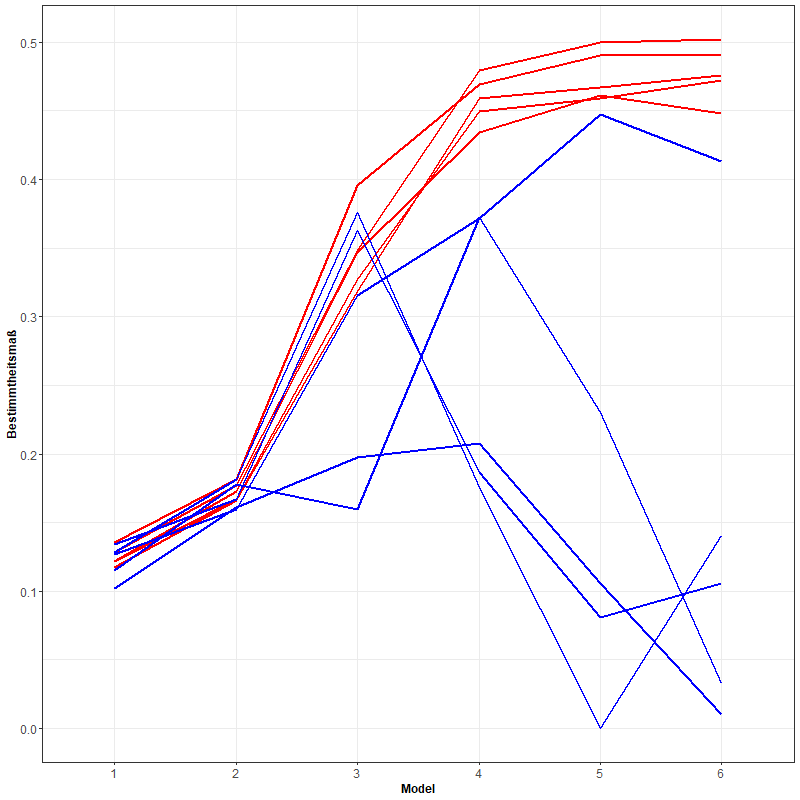
\includegraphics[width=\textwidth]{Plots/plot30.png}
	\caption{Feature Selection  Ergebnis der OLS Regression in 6 Modellen}
	\label{OLS_ModelSelection}
\end{figure}

Dass hier aber Overfitting auftritt ist kein Wunder, denn von dem Modell wird erwartet vorhersagen für, Vorhersagen für Stationen zu treffen, die im Trainingsdatensatz selbst nicht vorkommen und deswegen auch abweichende Charakteristiken aufweisen. Dies mach offensichlich, dass es ein leistungsfähigeres Modell braucht und bei allen folgenden Machine Learning Algorithmen muss berücksichtig werden, dass die Gefahr zum Overfitting relativ groß ist, und das vermutlich nie die Performance im Test Set erreicht wird, die sonst im Trainings Set erreicht wird. Die Abbildung \ref{tbl:OLS1} zeigt die Performance des endgültigen OLS Modells durch den Bestimmtheitswert und den root mean squarred error in jedem einzelnen Split. Split 3 zeigt die tatsächliche Tragweite des Overfitting, denn wo hier im Trainings Set ein RMSE 125 steht, nimmt der RMSE im Test Set astronomische Größen an. Dieses Beispiel zeigt auch den Vorteil der Cross Validation, denn dadurch, dass bei der Cross Validation 5 unterschiedliche Test Sets genutzt werden, steigt die Wahrscheinlichkeit, solche Modellfehler offenzulegen.\\
Es wird also deutlich, dass sich ein Log Lineares OLS Modell nicht dazu eignet, Vorhersagen für einen ganzen Stadtbereich zu machen. Weiterhin lohnt es sich nicht, hier weitere Versuche zu unternehmen. Und damit bleiben noch drei weitere Algorithmen übrig, wobei der nächst folgende die Support Vector Regression ist.

\begin{table}
	\csvautotabular[separator=semicolon]{Tables/Modell1OLS.csv}
	\caption{Performance des OLS Modells}
	\label{tbl:OLS1}
\end{table}

\section{Support Vector Regression}

Unter allen Methoden ist die Support Vector Regression jene, die noch die größten Ähnlichkeiten hat zur herkömmlichen nicht linearen OLS Regression. Vorteile waren aber, dass die Support Vector Regression weniger stark auf Ausreißer reagiert als die OLS Regression. Neben diesen Vorteil hat die Support Vector Regression den Nachteil, dass die Berechnung des Modells deutlich mehr Zeit in Anspruch nimmt und deswegen leistungsfähige Hardware erfordert.\\
Das R-Paket \glqq e1071\grqq, dass die passende Funktion bietet, stammte von \cite{e10712021}. R hat den Nachteil, dass es eine single threaded Sprache ist. Es spielt also keine Rolle, wie Leistungfähig die verwendete CPU ist, solange sich deren Leistung auf verschiedene CPU Kerne aufteilt. R nimmt zur Berechnung immer nur einen CPU Kern. Diese Limitation ließe sich umgehen mit dem Paket \glqq foreach\grqq von \cite{foreach} und \glqq doParallel\grqq auch von \cite{doParallel}, jedoch verhinderte das der zur Verfügung stehende RAM. R legt alle Daten mit denen ein Skript rechnet in den Arbeitsspeicher ab. Würden verschiedene Modelle gleichzeitig von verschiedenen CPU Kernen berechnet werden, dann müssten auch verschiedene Tests und Trainings Datensätze erstellt werden müssen und dies würde in Summe den zur Verfügung stehenden Arbeitsspeicher von nur 16 GB überlasten.\\
Eine Möglichkeit dieses Problem zu umgehen, wäre es z.B. auf Amazon Web Service zurückzugreifen, die Server zum trainieren von Machine Learning Algorithmen anbieten. Einfacher ist es jedoch, nur einen kleinen zufällig ausgewählten Anteil des Datensatzes zu verwenden. Dabei besteht natürlich die Gefahr, dass die Vorhersagekraft des Modells leidet, wenn man zu wenig Datenpunkte des Datensatzes verwendet. Der Datensatz beinhaltet insgesamt $4.472.091$ Beobachtungen. Davon wurden bei der OLS Regression jeweils 80 \% zum trainieren des Modells genutzt. Reduziert man diese Trainingsdaten weiter und wählt zufällige Beobachtungen aus, dann verhält sich die Performance des Modells so, wie in der Abbildung \ref{fig:TrainingsShareValidation2} zu sehen.

\begin{figure}%
	\centering
	\subfloat[\centering Bestimmtheitsmaß nach zum Training verwendeten Datensatzanteil]{{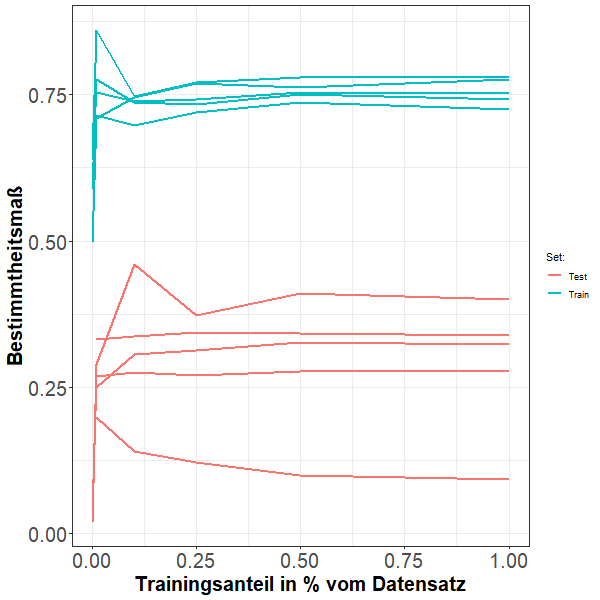
\includegraphics[width=6cm]{Plots/plot48.png} }}%
	\qquad
	\subfloat[\centering Bestimmtheitsmaß nach Trainingsdauer in Minuten]{{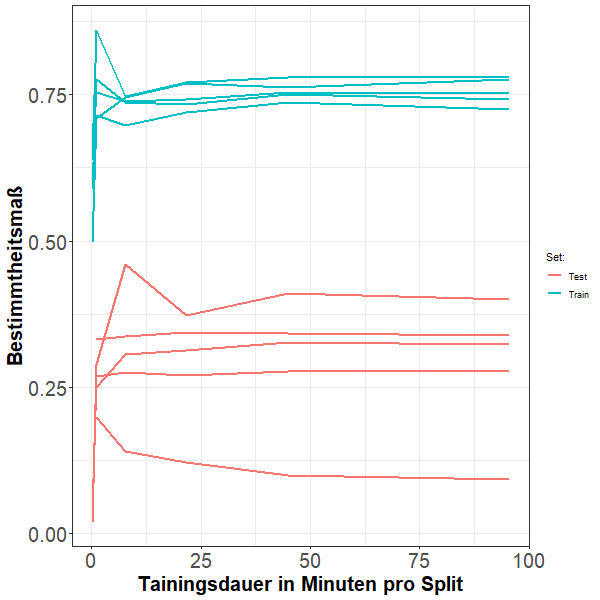
\includegraphics[width=6cm]{Plots/plot49.png} }}%
	\caption{Support Vector Regression Performance nach Anteil des Datensatzes}%
	\label{fig:TrainingsShareValidation2}%
\end{figure}

Dabei wurde das Modell einmal mit 0.001 \%, 0.01 \%, 0.1 \%, 0.25 \%, 0,5 \% und 1 \% getestet. Als erstes fällt auf, dass die Support Vector Regression bereits bessere Ergebnisse aufweist, als die OLS Regression, so steigt der Bestimmtheitswert für das Trainingsset auf bis zu 75 \% im Schnitt an, wo es zuvor noch um die 47 \% waren. Aber auch hier findet wieder Overfitting statt, denn der Bestimmtheitswert in den Test Sets steigt nur auf im Schnitt 25 \% an. Erhöht man den Anteil an Beobachtungen den man zum Training des Modells verwendet auf 0,25 \%, dann findet kaum noch eine nennenswerte Veränderung in der Performance statt. Nur die Dauer die zur Berechnung benötigt wird, steigt signifikant an. Nutzt man 0,25 \% der Daten zum Training, was ungefähr 9000 Beobachtungen entspricht, dann benötigt der Computer mit einer Intel Core i7-8750H CPU und 2,2 GHz Leistung im Schnitt 21 Minuten je Modell. Bei 1 \% verwendeter Daten, was ungefähr 37.800 Beobachtungen entspricht, benötigt die Berechnung bereits im Schnitt 90 Minuten pro Modell. Da jeweils 5 Modell trainiert werden auf 5 unterschiedlichen Cross Validation Sets und das das sechs mal zu unterschiedlichen Anteilen am Datensatz, hat die Erstellung der Ergebnisse in Abbildung \ref{fig:TrainingsShareValidation2} 14,2 Stunden benötigt.

\begin{figure}[!ht]
	\centering
	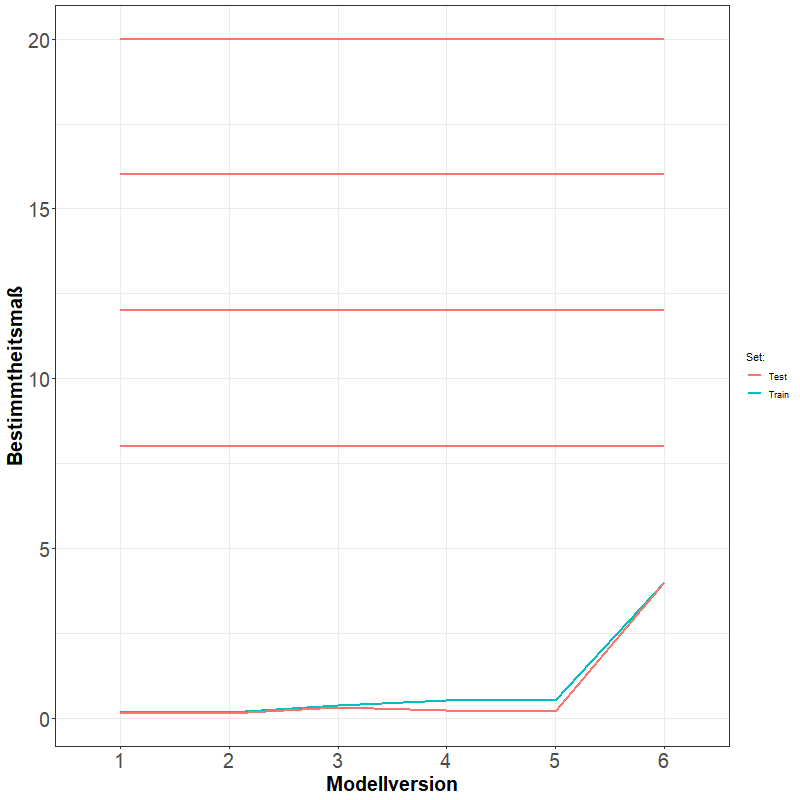
\includegraphics[width=\textwidth]{Plots/plot44.png}
	\caption{Support Vector Regression Ergebnis der RF Regression in 6 Modellen}
	\label{SVR_ModelSelection}
\end{figure}

Darüber hinaus kann man auch hier die Performance des Modells anhand der Auswahl der Variablen im Modell vergleichen. Auch hier werden im ersten Modell ausschließlich zeitliche Variablen verwendet, im zweiten kommen die fünf Wettervariablen hinzu, im dritten Variablen, die Demographie, Stadtausdehnung, Autobesitz und Fahradklima beschreiben, im vierten räumliche Variablen von Open Street Map, im fünften Modell Variablen zu den Straßentypen und im sechsten nicht lineare Variablen. Kubische Variablen sind dieses Mal in keinem Modell enthalten, weil dies zu einer Überlastung des Arbeitsspeichers führte. Alle Modelle wurden mit einem Trainingsanteil von 0,05 \% berechnet, also ungefähr 17.900 Beobachtungen. Den Vergleich zwischen den Modellen zeigt die Abbildung \ref{SVR_ModelSelection}. Diese zeigt deutlich, dass das geringste Maß an Overfitting im dritten Modell stattfindet, erst danach nimmt das Overfitting zu. Das dritte Modell allein ist jedoch von wenig Nutzen, denn ohne die räumlichen Variablen, gibt es keine Möglichkeit räumliche Unterschiede in der Vorhersage hervor zu eben, was der eigentliche Nutzen des Modells sein soll. So ist auch die Support Vector Regression nur wenig dazu geeignet zur räumlichen Vorhersage des urbanen Fahrradverkehrs.\\
Dies bestätigt auch ein weiterer Blick in die Tabelle \ref{tbl:SVR1}, die die Performance des endgültigen Support Vector Modells zeigt, mit allen Variablen, bis auf den kubischen. Im Vergleich zum OLS Modell sehen wir keine übermäßigen Ausreißer mehr im RMSE der Test Datensätze, aber die Performance verbessert sich nicht ausreichend genug, um damit vernünftige Aussagen treffen zu können.

\begin{table}
	\csvautotabular[separator=semicolon]{Tables/Modell2SVRradial.csv}
	\caption{Performance des SVR Modells}
	\label{tbl:SVR1}
\end{table}

\section{Random Forest Regression}\label{RF}

Die bisherigen Versuche ein schlüssiges Modell zu berechnen förderten leider nur unzufrieden stellende Ergebnisse hervor. Deswegen wird es Zeit leistungsfähigere Methoden zu verwenden. Das R Paket \glqq randomForest\grqq  von \cite{Liaw2002}. Ähnlich wie Support Vector Regressionen sind Random Forest deutlich rechenintensiver als eine OLS Regression. Deswegen wird auch hier nur ein Teil der Daten zum Training verwendet. Wie sich die Performance des Random Forest Models nach Anteil der zur Berechnung verwendeten Daten ändert, zeigt die Abbildung \ref{fig:TrainingsShareValidation1}, deren Berechnung insgesamt 9,35 Stunden benötigte. Dabei wird sichtbar, dass qualitativ wie auch quantitativ die Random Forests performanter sind, als die vorherhige Support Vector Regression. In Abbildung \ref{fig:TrainingsShareValidation2} war noch zu sehen, dass die Berechnung mit 1 \% der Daten ca 90 Minuten pro Modell benötigte. Hier sind es für 2 \% nur noch 80 Minuten.

\begin{figure}%
	\centering
	\subfloat[\centering Bestimmtheitsmaß nach zum Training verwendeten Datensatzanteil]{{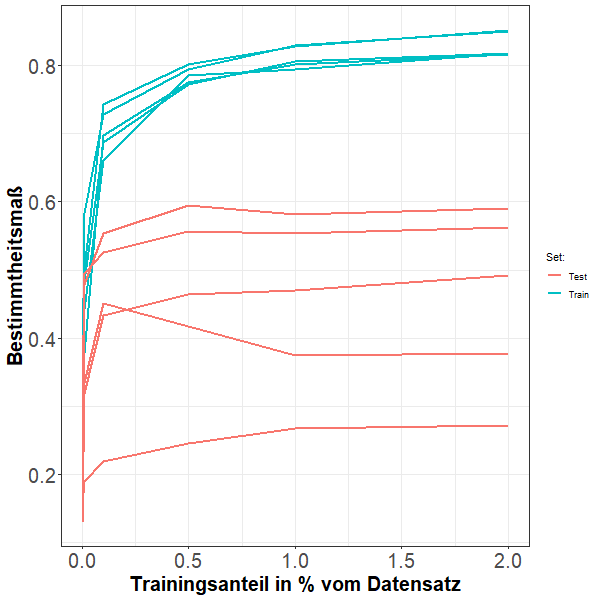
\includegraphics[width=6cm]{Plots/plot32.png} }}%
	\qquad
	\subfloat[\centering Bestimmtheitsmaß nach Trainingsdauer in Minuten]{{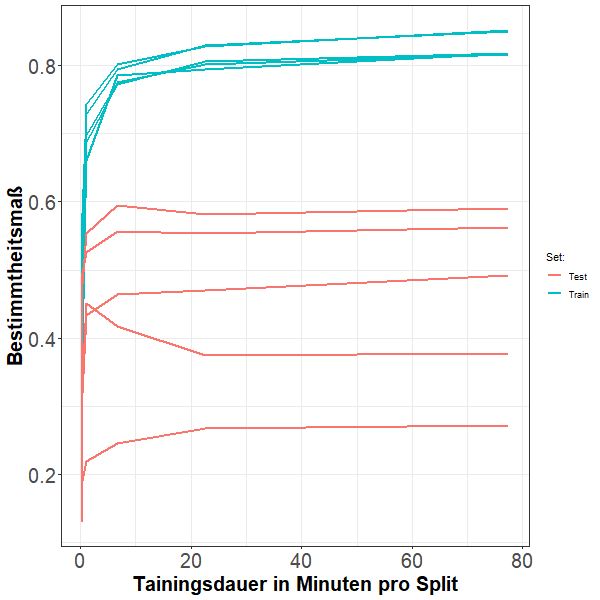
\includegraphics[width=6cm]{Plots/plot33.png} }}%
	\caption{Random Forest Performance nach Anteil des Datensatzes}%
	\label{fig:TrainingsShareValidation1}%
\end{figure}

Auch hier findet sich wieder Overfitting. Dennoch ist die Vorhersagesicherheit bedeutend besser als zuvor. Im Trainingsset erreicht das Random Forest Modell einen Bestimmtheitswert von 80 \% während die Support Vector Regression 75 \% maximal erreichte. Im Test Set sieht der Unterschied noch besser aus. Hier werden nun bis zu 60 \% erreicht. Zur Berechnung der Abbildung \ref{fig:TrainingsShareValidation1} wurden im Modell 500 Zufallsbäume verwendet. Diese Anzahl lässt sich variieren. Wie sich die Performance des Modells mit der Anzahl an verwendeten Zufallsbäumen verändert, zeigt die Abbildung \ref{fig:NTreeValidation1}, deren Berechnung 1,27 Stunden gebraucht hat. Dabei fällt schnell auf, dass das Maximum an Performance mit bereits relativ wenigen Zufallsbäumen bereits erreicht ist.

\begin{figure}%
	\centering
	\subfloat[\centering Bestimmtheitsmaß nach Anzahl der Zufallsbäume]{{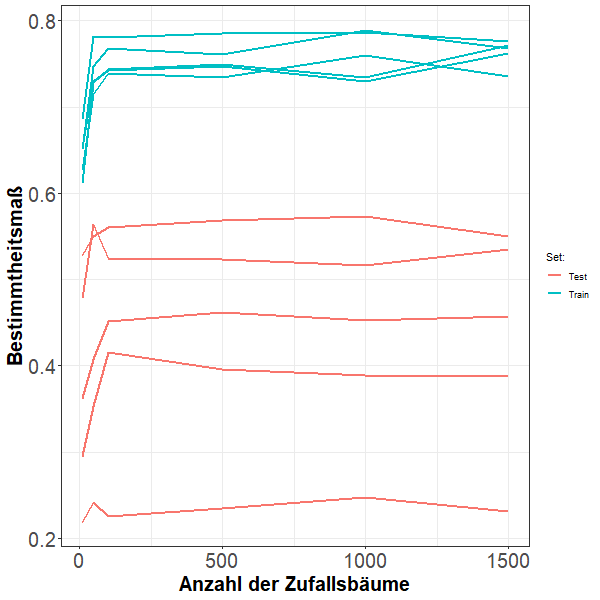
\includegraphics[width=6cm]{Plots/plot36.png} }}%
	\qquad
	\subfloat[\centering Bestimmtheitsmaß nach Trainingsdauer in Minuten]{{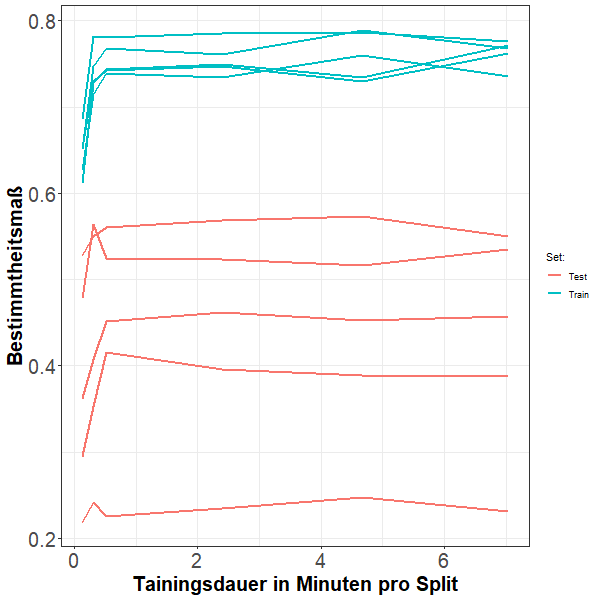
\includegraphics[width=6cm]{Plots/plot37.png} }}%
	\caption{Random Forest Performance nach Anzahl der Zufallsbäume}%
	\label{fig:NTreeValidation1}%
\end{figure}

Darüber hinaus bleibt nur noch der Vergleich von Modellen mit verschiedenen Variablen übrig. Dazu fand die selbe Modellauswahl wie im Abschnitt zur OLS Regression statt. Das heißt das Modell 1 greift auf Variablen zum Jahr, Monat, der Stunde, zum Wochenende, Nacht, und den Ferien- wie auch Feiertagen. Modell 2 fügt Wettervariablen hinzu. Modell 3 nutzt zusätzlich demographische Variabeln, Bevölkerungsanzahl, Fläche, Autobesitzrate, Immigrantenanteil und Fahrradklimaindex. Im Modell 4 kommen die Open Street Variablen hinzu. In den darauf folgenden Modellen kommen noch die nicht linearen Effekte hinzu. Zu sehen ist der Vergleich in der Performance der unterschiedlichen Modelle in der Abbildung \ref{RF_ModelSelection}. Einen ganz signifikanten Anstieg in der Performance ist zwischen Modell 2 und 3 zu sehen. Danach finden kaum große Änderungen in der Performance sowohl im Trainings Datensatz, als auch im Test Datensatz.

\begin{figure}[!ht]
	\centering
	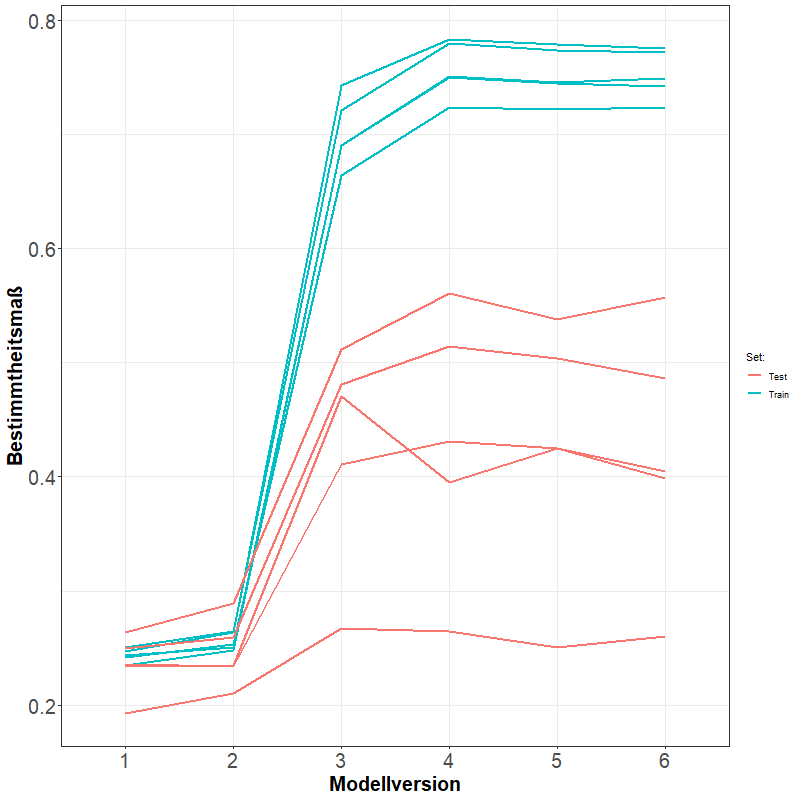
\includegraphics[width=\textwidth]{Plots/plot40.png}
	\caption{Feature Selection Ergebnis der RF Regression in 6 Modellen}
	\label{RF_ModelSelection}
\end{figure}

\begin{table}
	\csvautotabular[separator=semicolon]{Tables/Modell3RF.csv}
	\caption{Performance des RF Modells}
	\label{tbl:FR1}
\end{table}

Kombiniert man die so gewonnen Erkenntnisse zur Performance von Random Forest dann kommt man zu den Ergebnissen der Cross Validation in der Tabelle \ref{tbl:FR1}. Dieses Modell nutzte 0,5 \% der Trainingsdaten, 250 Zufallsbäume, verzichtet auf nicht lineare Variablen und benötigte zur Berechnung 24 Minuten. Im Test Datensatz erreicht das Random Forest Modell ein Bestimmtheitsmaß von 44,5 \%. Das ist mehr als dreimal so viel wie im OLS Modell und mehr als 1,5 mal so viel wie mit der Support Vector Regression. Auch wenn diese Werte bereits deutlich besser sind, als die der vorherigen Modelle, kann dies nicht darüber hinweg täuschen, dass sowohl die Höhe des Bestimmtheitsmaßes als auch des RMSE noch zu wünschen übrig lässt, doch in Anbetracht der schwierigen Aufgabe, die dieses Modell zu erfüllen hat, sind die Ergebnisse dennoch interessant, denn das Modell hat nur wenige Beobachtungsorte, auf deren Grundlage es Vorhersagen für ein ganzes Stadtgebiet treffen soll. Die letzte Methode, die nun noch übrig bleibt und die vielleicht in der Lage ist, noch bessere Vorhersagen zu treffen, ist das neuronale Netz.\\

Wendet man auf dieses Modell den zweiten Datensatz an, der Corona Daten beinhaltet und detailiertere Daten über die Straßenbeschaffenheit dann ändert sinkt das Bestimmtheitsmaß auf 41,16 \% im Test Set und der RMSE steigt leicht auf 137,43, während im Trainingsset die Werte besser aussehen mit einem Bestimmtheitsmaß von 81,52 \% und einem RMSE von 74,67. Das heißt hier ist das Overfitting sogar noch ein wenig größer. 

\section{Neuronales Netz}

Im Vergleich zu den vorherigen Methoden sind neuronale Netze die populärste Methode, vor allem bekannt für die verblüffende Präzesion ihrer Vorhersagen. Doch verblüffen die neuronalen Netze auch bei der Vorhersage des urbanen Radverkehrs? Das hängt vor allem von den vielen Variablen ab, die man bei einem neuronalen Netz einstellen kann. Zum einem kann man festlegen, wie viele Ebenen ein neuronales Netz haben soll und wie viele Knotenpunkte jede Ebene haben darf, die Informationen an die nächste Ebene weiter geben.\\
Leider ist jeder Durchlauf eines neuronalen Netzes sehr zeitintensiv. Diese Limitation erschwert den Vergleich in der Performance vieler verschiedener Modelle. So dauerte die Durchlaufzeit des Modells aus der Tabelle \ref{tbl:NN1} ganze 25,7 Stunden mit einer Anzahl an Beobachtungen von 20000. Würde man die Anzahl an Beobachtungen erhöhen, könnte das neuronale Netz unter Umständen bessere Vorhersagen treffen, dies würde jedoch auch die Durchlaufzeit erhöhen.\\
Grundsätzliche ist das Problem dieses Modells aber Overfitting. Von allen betrachteten Modellen ist hier das Overfitting am stärksten, betrachtet man die Unterschiede zwischen dem $R^2$ Wert im Trainings-Set der im Schnitt bei 93 \% liegt und im Test Set, wo der selbe Wert im Schnitt nur 9\% beträgt. Die Differenz könnte nicht größer sein.

\begin{table}
	\csvautotabular[separator=semicolon]{Tables/Modell4NN.csv}
	\caption{Performance des neuronalen Netzes}
	\label{tbl:NN1}
\end{table}

Das verwendete neuronale Netz nutzte sechs Neuronenreihen mit je 48, 26, 16, 8, 4 und 2 Neuronen. Hier müsste evaluiert werden, ob dieser Aufbau sich verbessern ließe. Die Anzahl von Trainingsschritten war auf 100000 begrenzt. Ein häufig auftretendes Problem war, dass das neuronale Netz keine Konvergenz zum Schwellenwert für die partielle Ableitung der Fehlerfunktion herstellen konnte, ganz gleich wie viele Trainingsschritte gemacht worden. Deswegen ist auch der Schwellenwert auf 0.025 hoch gesetzt. Dieser Wert ist zu hoch, war aber notwendig um überhaupt Ergebnisse hervor zu bringen. Je Modell wurden drei wiederholte Trainingsansätze genutzt. Diese Anzahl könnte man noch erhöhen um mehr Generalisierung zu erzielen.\\
Im Vergleich aller Modelle brachte das Random Forest Modell die besten Vorhersagen hervor. Im weiteren Verlauf wird also immer von dem Random Forest Modell die Rede sein.

\section{Model Projektion}

In den vorangegangenen Sektionen wurden die Ergebnisse vier verschiedener Machine Learning Modelle vorgestellt. Dies waren die Ergebnisse der OLS Regression, der Support Vector Regression, von Random Forest und die Ergebnisse eines neuronalen Netzes. Dabei haben die Ergebnisse des Random Forests die Ergebnisse mit der höchsten Plausabilität geliefert getestet durch die Cross Validation.\\
Dieses Modell lässt sich nun dazu nutzen, Vorhersagen auf ein ganzes Straßennetz zu projezieren. Die Daten des Straßennetzes stammen wiederum von Open Street Map. Der erste Schritt ist es, einen Kartenbereich auszuwählen mithilfe zweier Koordinaten wie in Code \ref{code:projection1}. Dabei ist anzumerken, je größer dieser Kartenausschnitt sein soll, desto höher ist natürlich auch die Datenlast. Bei ganzen Stadtgebieten ist es zu empfehlen, nur einzelne Straßentypen auszuwählen, oder den Prozess in mehrere Ausschnitte aufzuteilen. Die Koordinaten werden in \lstinline|myLocation| gespeichert. Der hier dargestellte Code würde einen Code Ausschnitt des Ringbereichs in Münster auswählen.

\begin{lstlisting}[caption={Wahl des Kartenausschnitts},label=code:projection1]
myLocation <- c(7.597514856738869,51.94573812395569,   
		7.652382675482133,51.9756143280805)
		
q <- myLocation %>% 
opq() %>%
add_osm_feature("highway")

streets <- osmdata_sf(q)
\end{lstlisting}

Danach wird eine Anfrage an Open Street Map gestellt, die Daten des Typs "highway" im angegebenen Kartenbereich zu downloaden. Dieser Prozess ähnelt dem Prozess, wie wir ihn im Abschnitt \ref{OMSDATA} kennen gelernt haben.\\
Darauf folgend müssen die ausgelesenen Daten in einem Format gespeichert werden, die in einen Datensatz für das Modell und zur Kartenprojektion verwendet werden könnten. Zunächst bestehen die Open Street Map Daten aus verschiedenen Straßenlinien, deren Koordinaten in \lstinline|streets$osm_lines$geometry| gespeichert sind. Jede Straßelinie besteht aus mehreren und zusammenhängenden Vektoren, und diese Vektoren bestehen je aus zwei Koordinaten. Zunächst müssen die einzelnen Vektoren der Straßenlinien voneinander getrennt werden, damit jeder Vektor mit einem seiner beiden Koordinaten im Datensatz wie eine Zählstation behandelt werden kann. Dabei wird die erste Koordinate in \lstinline|streetPositions$Lon| und \lstinline|streetPositions$Lat| gespeichert und die zweite Koordinate in \lstinline|streetPositions$Lon2| und \lstinline|streetPositions$Lat2|. Aufgrundlage der ersten Koordinaten können dann Vorhersagen getroffen werden. Der Code \ref{code:projection2} zeigt diesen Prozess.\\
Dabei werden zwei \lstinline|for|-Loops verwendet.

\begin{lstlisting}[caption={Wahl des Kartenausschnitts},label=code:projection2]
for(i in 1:length(streets$osm_lines$geometry)){
	l = length(streets$osm_lines$geometry[[i]])
	
	for(j in 1:(length(streets$osm_lines$
		geometry[[i]])/2 - 1)){
	
		streetPositions$Lon[k]=streets$osm_lines
		$geometry[[i]][j]
		streetPositions$Lat[k]=streets$osm_lines
		$geometry[[i]][l/2+j]
		streetPositions$Lon2[k]=streets
		$osm_lines$geometry[[i]][j+1]
		streetPositions$Lat2[k]=streets
		$osm_lines$geometry[[i]][l/2+j+1]
	}
}
	
\end{lstlisting}

Der erste \lstinline|for|-Loop geht alle Straßenlinien durch. Der zweite \lstinline|for|-Loop geht alle Vektoren innerhalb der jeweiligen Straßnenlinie durch. Innerhalb der zweiten Schleife werden dann die Einzelwerte der jeweiligen Koordinate in dem Dataframe \lstinline|streetPositions| gespeichert, dieser wird darauffolgend als Grundlage für die Vorhersagen genutzt. Die Variablen die zu Vorhersagen benötigt werden, werden ähnlich wie in Kapitell \ref{Datensatz} gebildet. Darüber hinaus kann man einzelne Faktoren auch überschreiben, um hypottetische Fälle zu betrachten.\\
Hat man nun einen solchen Datensatz, der die Vorhersagen des jeweiligen Modells enthällt, ist die beste und anschaulichste Präsdentation dieser Ergebnisse eine graphische Übersicht des Straßennetzes mit farblicher Markierung der Fahrradauslastung, wie sie für die in Abschnitt \ref{RF} zwei verschiedenen Random Forest Modell in Abbildung \ref{fig:MunsterRing} zu sehen sind. Zusätzlich worden die im Datensatz enthaltenen Zählstellen als Ringe auf der Karte dargestellt, deren farblich die durchschnittliche Radauslastung an der jeweiligen Zählstation markiert.

\begin{figure}%
	\centering
	\subfloat[\centering nach Modell 1]{{\includegraphics[width=10.5cm]{Plots/Münster_Ring_Modell1.png} }}%

	\subfloat[\centering nach Modell 2]{{\includegraphics[width=10.5cm]{Plots/Münster_Ring_Modell2.png} }}%
	\caption{Räumliche Modell Projektion: Modellvergleich}%
	\label{fig:MunsterRing}%
\end{figure}

Wie in der Abbildung \ref{fig:MunsterRing} unterscheiden sich beide Modelle sehr stark. Während in der Abbildung zum ersten Modell zu sehen ist, dass das Aufkommen des Radverkehrs in der räumlichen Vorhersage flächenmäßig relativ gleichverteilt ist aber konzentriert auf das Stadtzentrum, ist die Vorhersage des zweiten Modells weniger gleichmäßig. In der zweiten Abbildung ist ein stärkeres Rauschen zu sehen. Dabei ergibt das Rauschen des Vorhersage an manchen Stellen Sinn, an anderen jedoch weniger Sinn. Was nützlich an Modell 2 ist, dass bestimmte einzelne Straßenzüge stärker betont werden, vorallem auch spezifische Kreuzungen im Bereich der Ringstraße Münsters. Es fallen z.B auf die Kreuzung Niedersachsenring/Bohlweg, Niedersachsenring/Gartenstraße, Kaiser-Wilhelm-Ring/Warendorfer Straße oder auch die Kreuzung Kolde-Ring/Weseler Straße. Dies sind jedoch auch wichtige Verkehrsadern der Stadt Münster, dass eine Radverkehrsdichte im Bereich der Ring Straßen herrschen muss, scheint trivial. Doch kann das Modell auf vorhersagen, dass dies nicht im ganzen Ring Bereich so sein muss. Für den Nordwesten des Ringbereichs sagen beide Modelle eine niedrige Radverkehrsdichte hervor. Ohne einer weiteren Zählstation lässt sich dies nicht abschließend prüfen, wir kennen jedoch auch die gemessene Validität der Modelle. Darüber hinaus macht das zweite Modell für einige Nebenstraßen sehr hohe Vorhersagen. Diese erscheinen nicht plausibel. Eine Möglichkeit wäre es, diese Nebenstraßen und Parkgassen in der Anzeige auszuschließen, so wie es z.B. auch mit Gehwegen und Fußgängerzonen geschehen ist. Die graphische Ausgabe der Modellvorhersagen lässt sich also noch verbessern.\\
Mit der Absicht die Validität des Modells noch weiter zu erhöhen ist ein drittes Modell entstanden, dass alte und neue Straßentypen Variablen mit in das Modell aufnimmt, zusätzlich noch mehr nicht lineare Effekte und eine größere Stichprobenmenge von 80000 Beobachtung nutzt. Dieses dritte Modell hat in der Berechnung 28 Stunden benötigt. Die Ergebnisse zeigt die Tabelle \ref{tbl:RF3} und die Abbildung \ref{Munster}. Graphisch ist dieses Modell fast identisch zum zweiten Modell. Da Modell 2 und 3 brauchbarere Vorhersagen machen, weil beide einzelen Straßenzüge hervorheben und weil Modell 3 eine höhere Treffsicherheit als Modell 2 hat und mit mehr Beobachtungen trainiert worden ist, wird für weitere Vorhersagen Modell 3 verwendet.

\begin{table}
	\csvautotabular[separator=semicolon]{Tables/Modell3RFnewDataset2.csv}
	\caption{Performance des dritten RF Modells}
	\label{tbl:RF3}
\end{table}

\begin{figure}[!ht]
	\centering
	\includegraphics[width=\textwidth]{Plots/Münster_Ring_Modell3.png}
	\caption{Feature Selection Ergebnis der RF Regression in 6 Modellen}
	\label{Munster}
\end{figure}

\begin{figure}%
	\centering
	\subfloat[\centering Hamburg]{{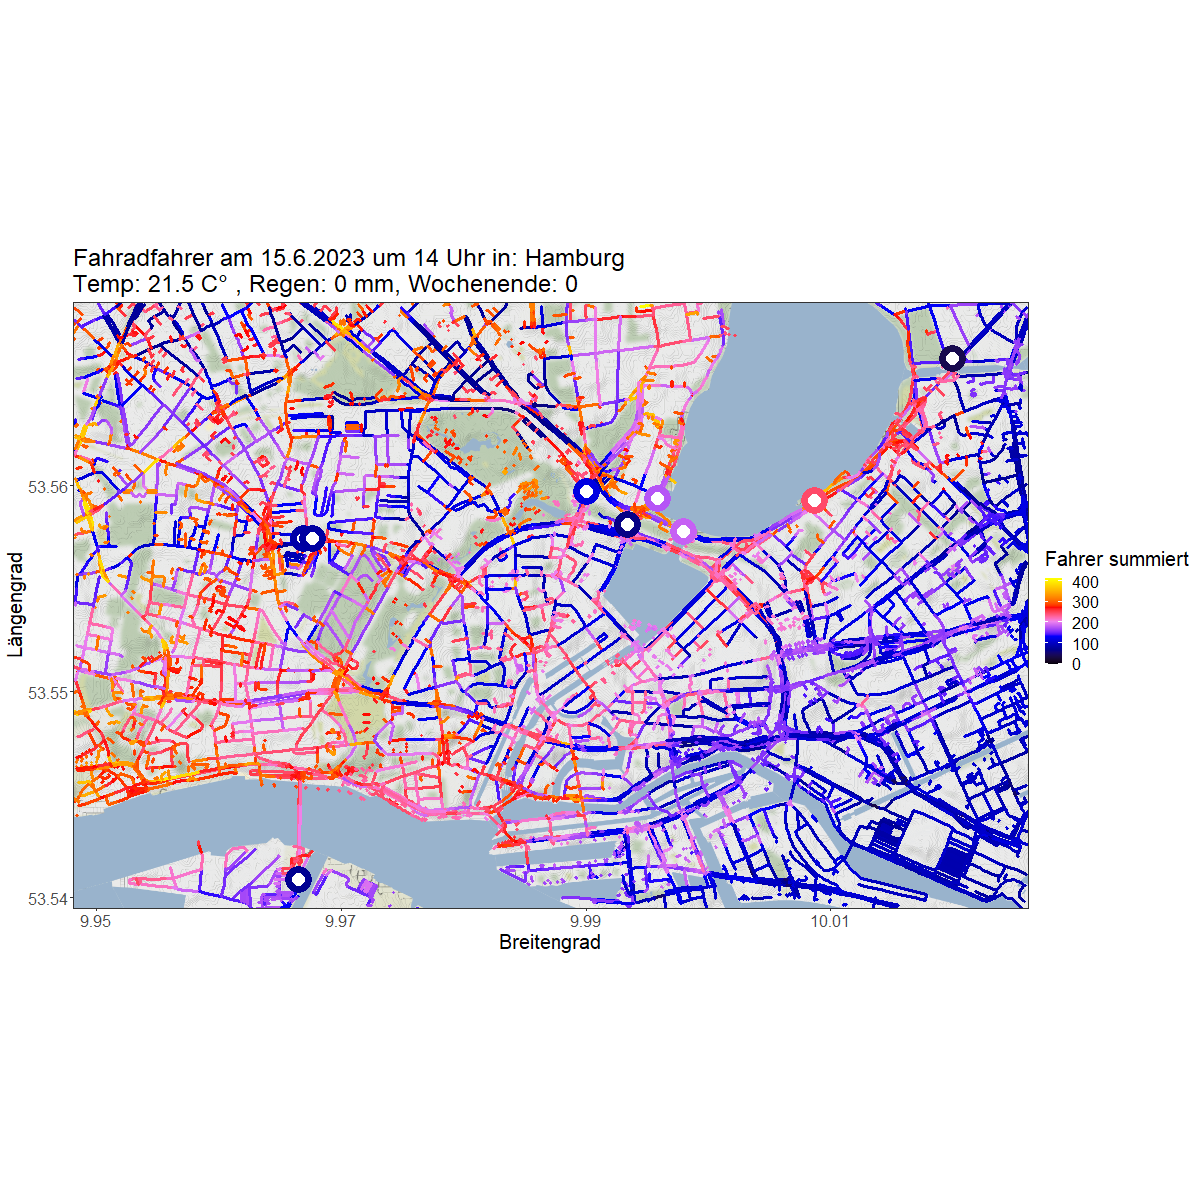
\includegraphics[width=10.5cm]{Plots/Hamburg.png} }}%
	
	\subfloat[\centering Leipzig]{{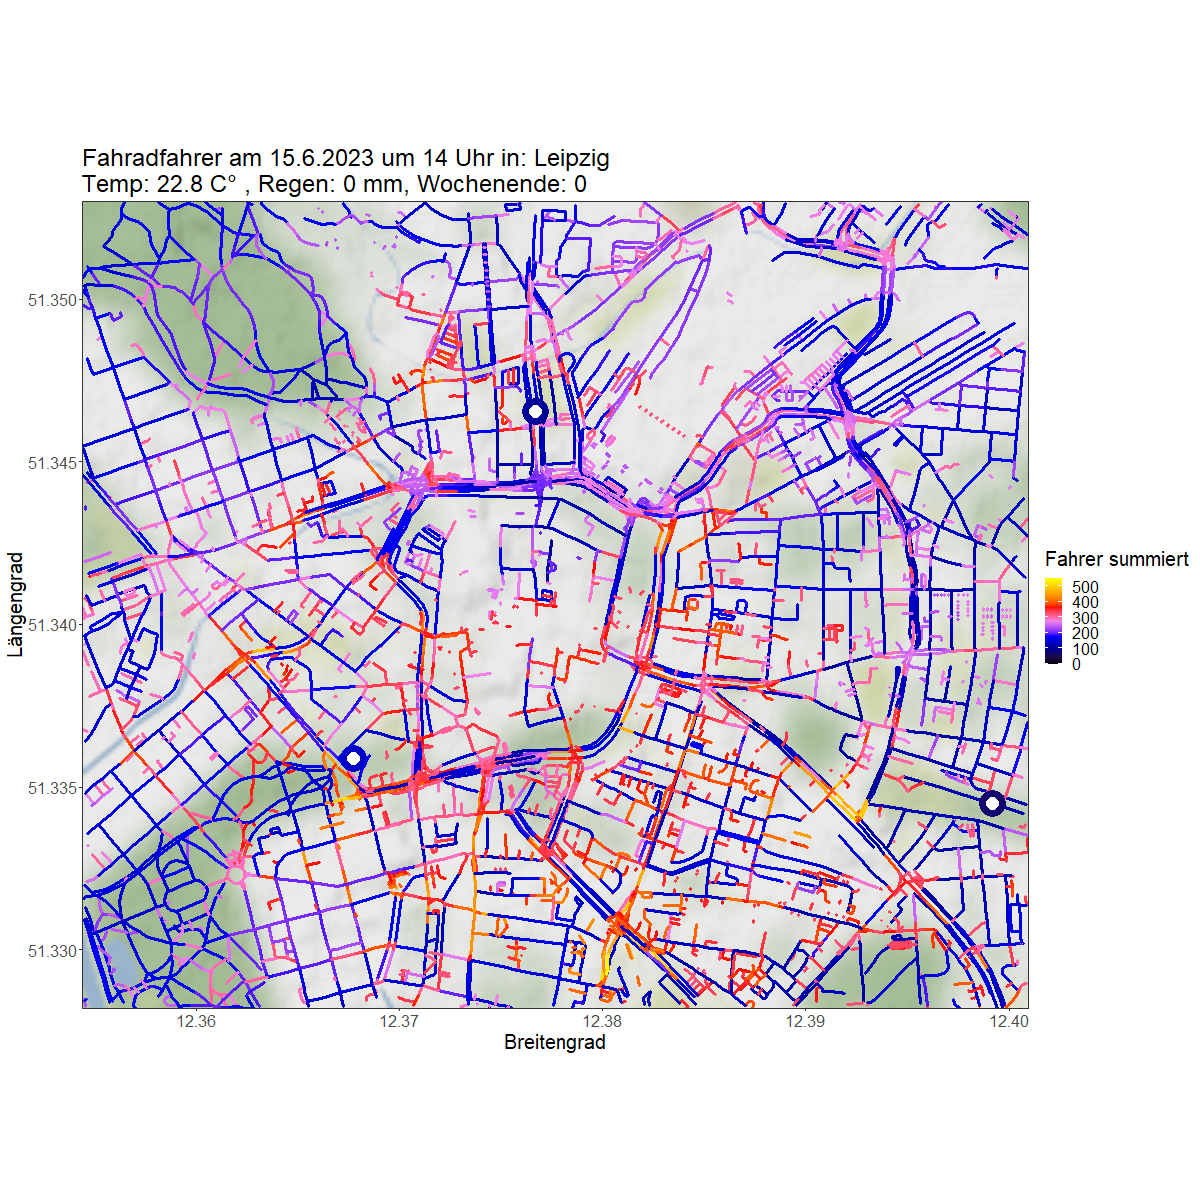
\includegraphics[width=10.5cm]{Plots/Leipzig.png} }}%
	\caption{Modellprojektionen in Hamburg und Leipzig}%
	\label{fig:HamburgundLeipzig}%
\end{figure}

\begin{figure}%
	\centering
	\subfloat[\centering Mannheim]{{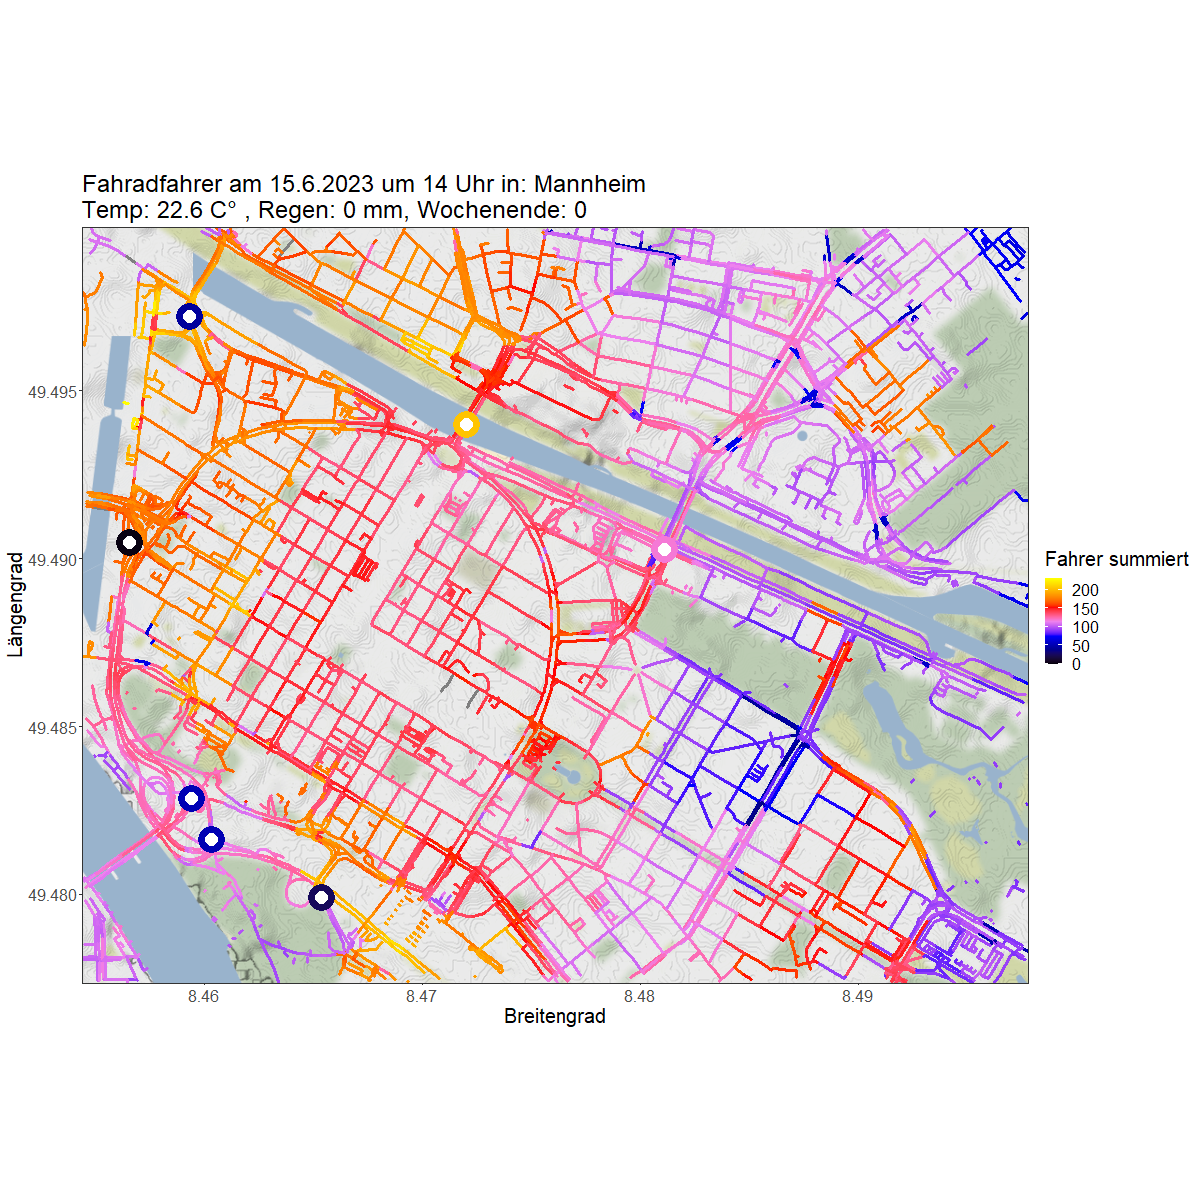
\includegraphics[width=10.5cm]{Plots/Mannheim.png} }}%
	
	\subfloat[\centering Oberhausen]{{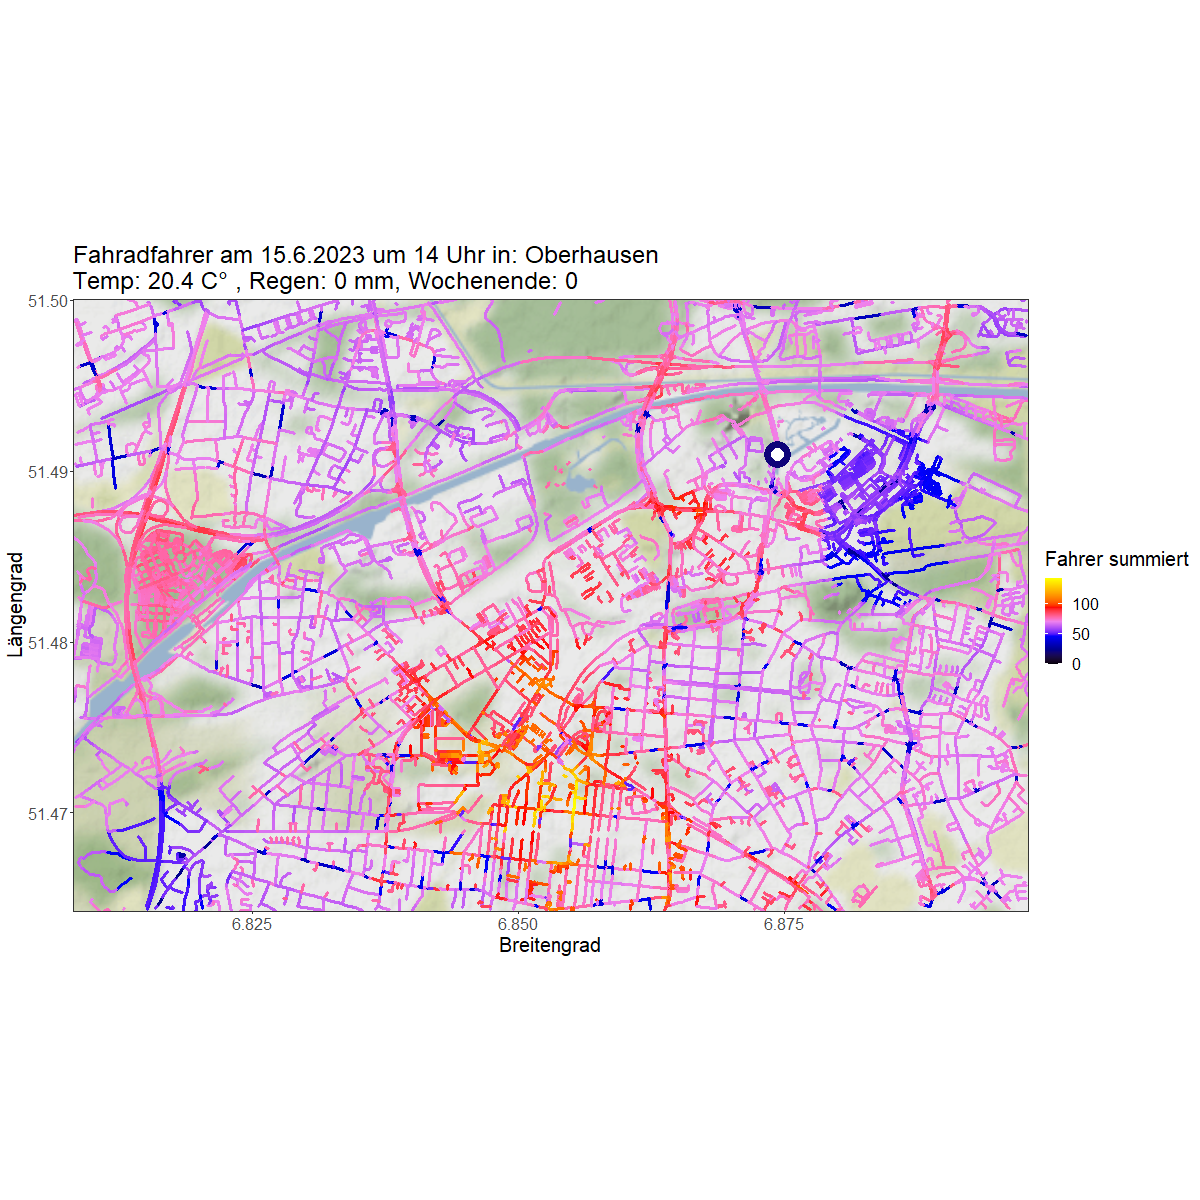
\includegraphics[width=10.5cm]{Plots/Oberhausen.png} }}%
	\caption{Modellprojektionen in Mannheim und Oberhausen}%
	\label{fig:MannheimundOberhausen}%
\end{figure}

Die Abbildungen \ref{fig:HamburgundLeipzig} und \ref{fig:MannheimundOberhausen} zeigen beispielhaft die Verkehrsprognosen für Hamburg, Leipzig, Mannheim und Oberhausen. Es wird offensichtlich, dass das Modell sich dem Verkehrsniveau der Städte anpasst. An manchen Stellen scheint das Modell das Verkehrsaufkommen zu überschätzen, vergleicht man es zu den markierten Stationen. Die markierten Stationen zeigen jedoch nur den Durchschnitt über alle Messnungen hinweg an. Da die Modellprojektionen ein Datum in der Zukunft gewählt haben im Sommer, an dem Spitzenwerte auftreten ist hier ein Vergleich schwierig.\\
Um das Modell einem besonderen Stresstest zu unterziehen, muss Vorhersagen für eine ganze Stadt machen, die dem Modell unbekannt ist, Messwerte zu dieser Stadt aber vorliegen. Weil im Verlauf der Masterarbeit die Zählwerte aus Dresden erst spät zugänglich waren, konnten diese Daten selbst nicht mit in das Modell einfließen, sind nun aber nützlich für eine zusätzliche Validierung. Diese Daten aus Dresden stammen von 8 verschiedenen Zählstationen von 2018 bis 2021 und umfassen insgesamt 261576 Beobachtungen. Das Modell schätzt hier in Dresden über alle Beobachtungen den Durchschnitt der Radfahrer auf 40.95. Der tatsächliche Durchschnitt entspricht jedoch 83.66 und ist somit doppelt so hoch. Der vorhergesagte Medianwert liegt bei 27.06 und der tatsächliche Medianwert liegt bei 43. Das Modell scheint also den Verkehr in Dresden zu unterschätzen. Der RMSE für diese Daten liegt bei 115.76, was im Bereich der vorherigen Evaluationen lag, jedoch liegt das Bestimmtheitsmaß $R^2$ nur noch bei 0.06.\\
Dies sind Hinweise darauf, dass Modellprojektionen in unbekannten Städten unzuverlässig sind. Diese Vermutung bestätigt sich beim graphischen Modelloutput in Abbildung \ref{Dresden}. Dieser Modelloutput zeigt im Zentrum Dresdens wenig Verkehr in Randbezirken mehr und wirkt deswegen unglaubwürdig. In Verbindung mit den Validierungswerten des RMSE und des Bestimmtheitswertes sowie des unterschiedlichen Medians und Durchschnitts in vorhergesagten und tatsächlichen Verkehrsdaten, zeigt das Dresdner Beispiel die Grenzen des Modells. Wo die Modellprojektionen für dem Modell bekannte Stationen glaubwürdig validiert werden konnten, sind die Modellvorhersagen für die unbekannte Stadt Dresden unglaubwürdig.

\begin{figure}[!ht]
	\centering
	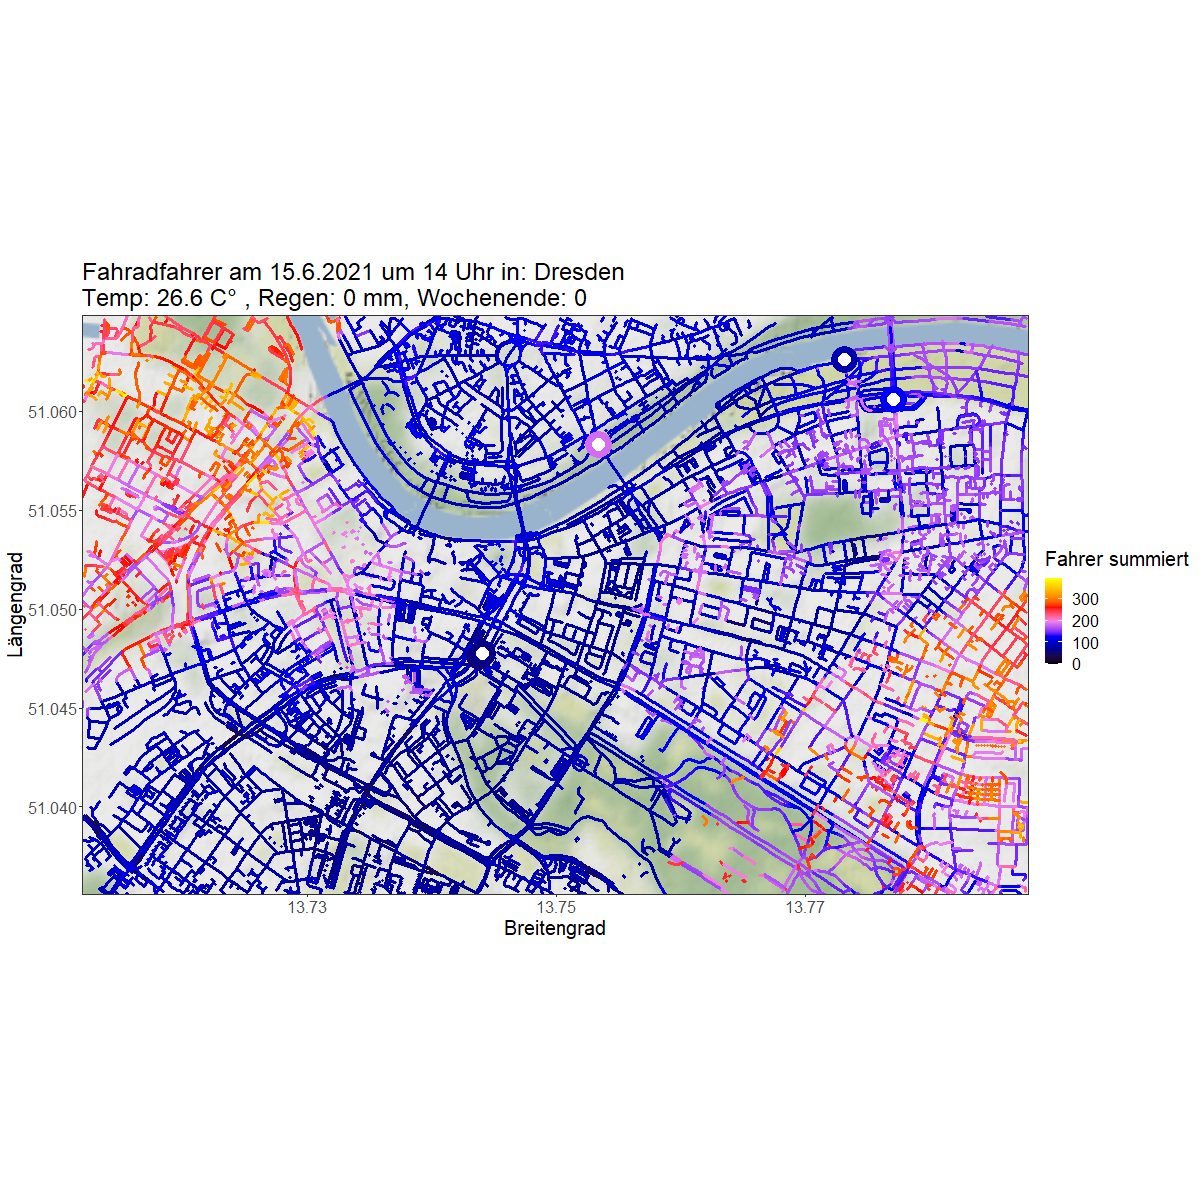
\includegraphics[width=\textwidth]{Plots/Dresden.png}
	\caption{Modellprojektionen in Dresden}
	\label{Dresden}
\end{figure}

\section{Räumliche Korrelation zu Verkehrsunfällen}

Auch wenn wie im vorherigen Abschnitt dargestellt die Vorhersagen für unbekannte Städte unbrauchbar sind, ist die Verwendung für die 22 deutschen Städte, die im Modellsatz vorkommen denkbar. Eine weitere interessante Frage ist, ob die Modellvorhersagen räumlich mit Radverkehrsunfällen korrelieren. Sollte dies der Fall sein, könnte dies das Modell zum einem bestätigen, aber auch dabei helfen Straßenstellen ausfindig zu machen, die über ihr Verkehrsniveau hinaus gefährlich sind durch falsches Straßendesign.\\
Für den Fall in Münster stellt die Organisation Code for Münster Verkehrsunfalldaten zur Verfügung (Quelle: \url{https://crashes.codeformuenster.org}, Stand: 9.2.2023). Diese Daten aus Münster reichen von 2008 bis 2018 und umfassen 6676 Unfälle bei denen Fahrräder inovolviert wurden und die Koordinaten mit aufgezeichent worden. Diese Daten lassen sich clustern, in dem man jedem Punkt im Straßennetz zu ordnet, wie viele Unfälle in einem gegebenen Radius geschehen sind. Für einen Radius von 64 Metern zeigt dies die Abbildung \ref{fig:Unfallkarten}b. Nach dem man man dem Straßennetz die jeweiligen Unfallzahlen zu gewiesen hat, kann man auf dieses Straßennetz Modellvorhersagen zur Radverkehrsdichte treffen, um die räumliche Korrelation der Radverkerhsvorhersage des Modells mit den Unfalldaten zu messen. Dabei bildet jeder Straßenknotenpunkt eine Beobachtung da, mit den geclusterten Unfalldaten und der Modellvorhersage, die auf den 15. Juni 2018 14 Uhr datiert.\\

\begin{figure}%
	\centering
	\subfloat[\centering Beobachtungen nach Unfällen und Radverkehr]{{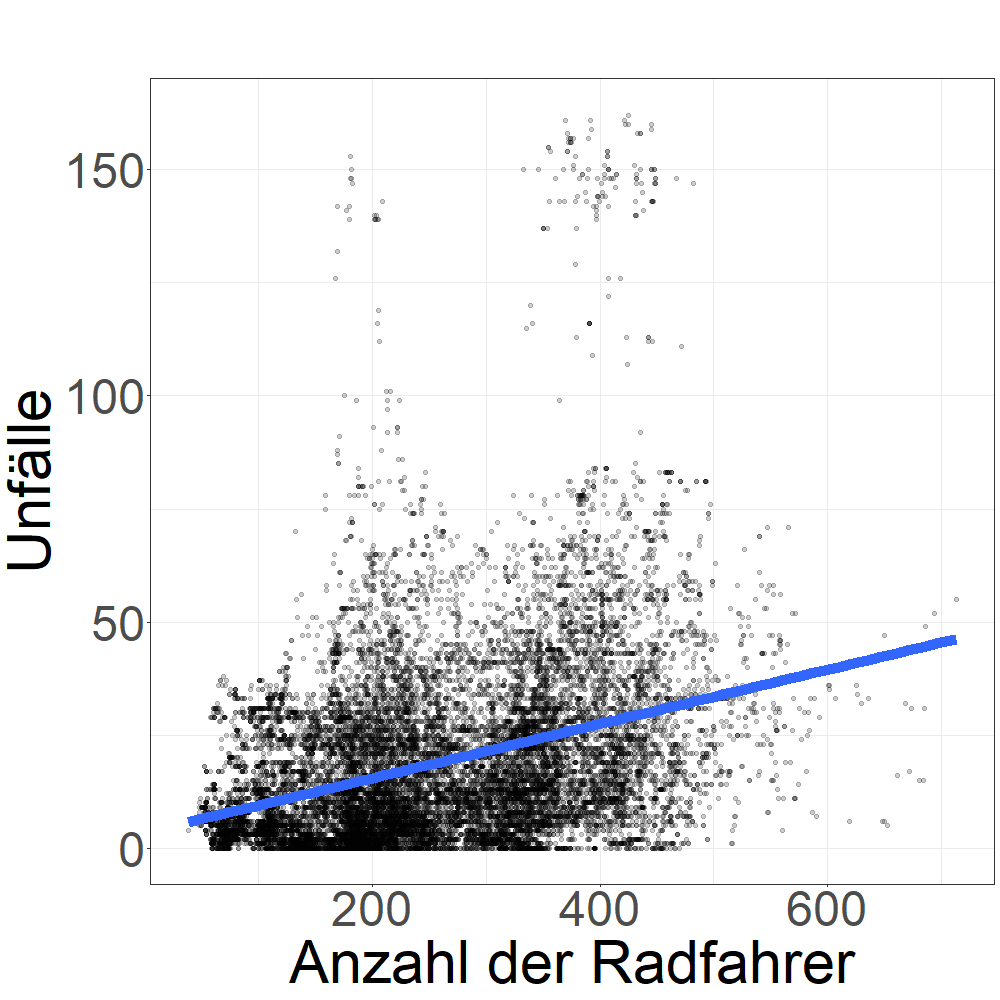
\includegraphics[width=6cm]{Plots/Korrelationsgraf128.png} }}%
	\qquad
	\subfloat[\centering Korrelation nach Unfallradius]{{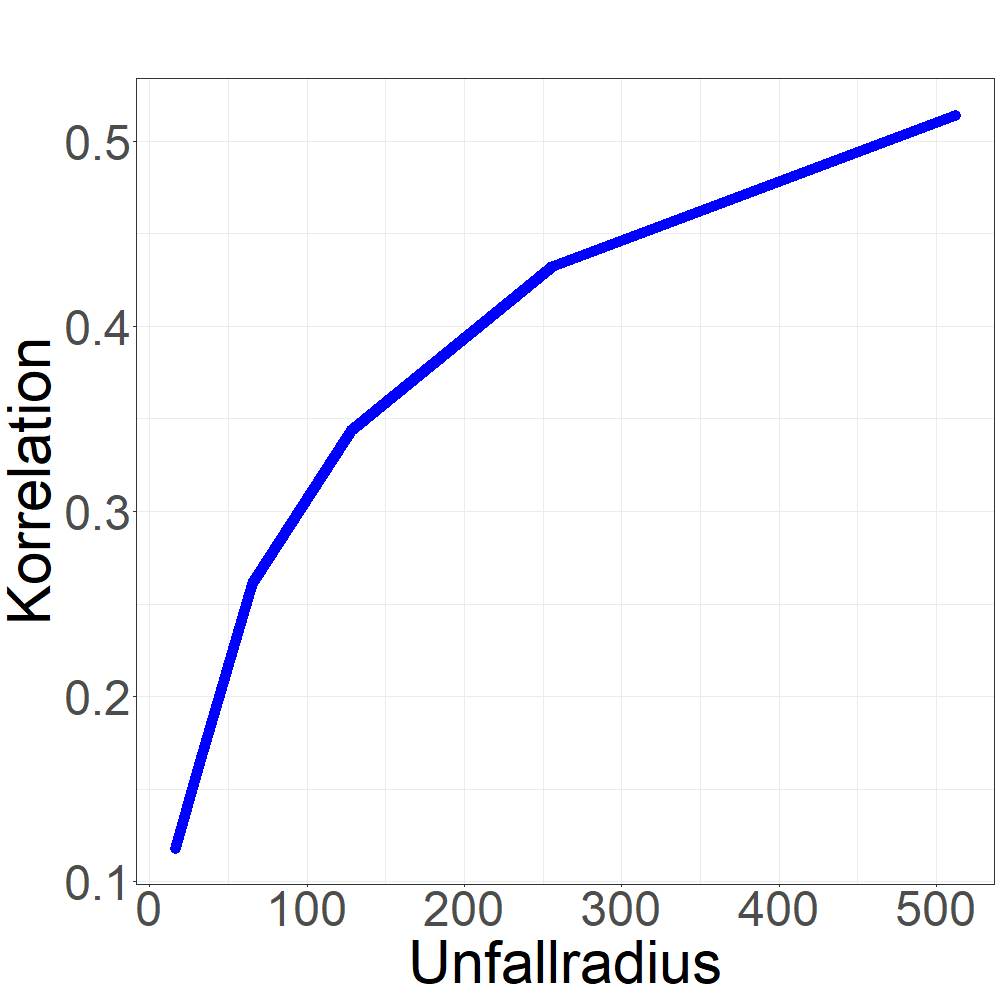
\includegraphics[width=6cm]{Plots/Korrelation.png} }}%
	\caption{Räumliche Korrelation von Unfällen und Radverkehr}%
	\label{fig:UnfallKorrelatoon}%
\end{figure}

Diese Beobachtungen sind dargestellt in der Abbildung \ref{fig:UnfallKorrelatoon}a. Dabei zeigt sich ein ansteigender korrelativer Zusammenhang. Beim Clustern der Unfalldaten lässt sich bestimmen in welchem Radius um den Straßenpunkt herum die Unfälle kummuliert werden. Dabei lässt sich beobachten, dass je höher dieser Radius ist, desto höher ist die Spearman Korrelation dieser Daten, auch zu sehen in Abbildung \ref{fig:UnfallKorrelatoon}b. Bei einem Unfallradius von 8 Metern beträgt die Spearman Korrelation 0,118 und bei einem Unfallradius von 512 Metern beträgt die Spearman Korrelation 0,514. Diese Korrelationen sind jeweils statistisch signifikant. Dieser Zusammenhang bestätigt das Modell vorerst weiter.\\



Jedoch zeigt die Karte \ref{fig:Unfallkarten}a auch Abweichungen. Diese Karte zeigt farblich markiert die Radverkehrsdichte, die das Modell vorhersagt und markiert durch die Transparenz der Straßenlinien die Unfalldichte des Radverkehrs. An vielen Stellen korreliert beides, wie z.B. am Ludgeri Kreisel südlich der Altstadt. Dies ist die Stelle in Münster mit den meisten Radunfällen und auch mir einem hohem Radverkehr. Jedoch zieht sich eine weitere hohe Unfalldichte über die Länge der Hammerstraße hinweg, die vom Ludgerikreisel in Richtung Süden wegführt. Das Modell sagt hier aber eine geringe Verkehrsichte vorher. Auch im Nordosten im Bereich der Ringstraße stehen Unfalldichte und Radverkehrsdichte in Dissonanz. Dafür kann es zwei Erklärungen geben. Entweder trifft das Modell falsche räumliche Vorhersagen an diesen Stellen, oder aber diese Verkehrsstellen, sind besonders gefährlich und führen auch mit weniger Verkehr zu vielen Verkehrsunfällen.

\begin{figure}%
	\centering
	\subfloat[\centering Radverkehr und Unfälle]{{\includegraphics[width=10.5cm]{Plots/Korrelationskarte_Münster.png} }}%
	
	\subfloat[\centering Unfallkarte]{{\includegraphics[width=10.5cm]{Plots/Unfallkarte_Münster.png} }}%
	\caption{Karten zu Unfällen und Radverkehr}%
	\label{fig:Unfallkarten}%
\end{figure}

\chapter{Diskussion}

Die Forschungsfrage dieser Masterarbeit war, ob es möglich ist, ein räumliches Modell zu entwickeln, das für ein vollständiges Straßennetz oder für ausgewählte flexible Knotenpunkte zu bestimmten Zeiten Vorhersagen zum Fahrradverkehr machen kann und lassen diese auch zusätzlich die gefährlichsten Stellen für Fahrradunfälle erkennen? Das Resultat dieser Masterarbeit ist das zuvor viel beschriebene Modell. Um die Forschungsfrage zu beantworten, muss der Wert des Modells diskutiert werden und so wie es die Absicht der Masterarbeit war im besonderen Bezug zur kommunalen Infrastruktur Planung und Unfallvermeidung.\\
Der schwierigste Aspekt in der Modellierung war die räumliche Interpolation einzelner Zählstationen, von denen es nur begrenzt viele gibt. Ein grundsätzliches Problem dabei ist, dass Zählstationen oft nicht zufällig gesetzt werden sondern mit Absicht an Stellen, wo man einen hohen Verkehr erwartet. Dies verletzt aber die Annahme von unabhängig und gleichverteilten Beobachtungen. Dies ist der Grund für das massive Overfitting, welches den Modellen allen zu Grunde liegt. Jedoch Ließ sich durch Cross Validation dieses Overfitting aufdecken. Der Wert der für die externe Validität bemessen wurde steht. Hinter ihm verstecken sich keine weitere Überraschungen von Verzerrungen, die einem in der Anwendung des Modells noch begegnen können. Das heißt mithilfe der Cross Validation lässt sich die Performance des Modells getreu beurteilen.\\
Die übrig bleibende Frage ist, ob diese Performance der Anwendung zur Verkehrsplanung und zur Unfallvermeidung ausreicht. Auszuschließen ist die Verwendung für out of Sample Städten. Das heißt zur Vorhersage braucht das Modell eine Anzahl von Zählstellen, um schlüssige Vorhersagen zu treffen, wie das Beispiel aus Dresden gezeigt hat. Davon abgesehen liefert das Modell jedoch schlüssige Antworten darauf, wie sehr sich der Verkehr in einzelnen Stadtteilen unterscheidet und welche Kreuzungen am stärksten frequentiert werden und zeigt somit auch den eventuellen Bedarf an Radverkehrsinfrastruktur. Auch ein Abgleich von Verkehrsunfallsdaten kann zeigen, ob einzelne Hotspot für Fahrradunfälle mit dem Radverkehr korrelieren, oder einfach nur signifikant gefährlich sind. Solche Hinweise müssen jedoch einzeln geprüft werden.\\
Was nur begrenzt möglich ist, ist eine Vorhersage beruhend auf die Veränderung der Infrastruktur, die dem Modell als Daten zugrundeliegen. Im Modell sind Variablen wie die Anzahl von Geschäften und Stationen des öffentlichen Nahverkehrs in der Umgebung enthalten. Dabei wird es sich aber um rein korrelative und nicht kausale Zusammenhänge handeln, weil diese Variablen selbst auf die Verdichtung des Verkehrs hinweisen. Ändert man also die Anzahl an Bus Stationen in einem Bereich, hat dies im Zweifel keine Auswirkungen auf den Radverkehr, nur  weil der Radverkehr ähnlich verdichtet ist, wie der öffentliche Nahverkehr im Zentrum einer Stadt.\\
Kausale räumliche Einflussfaktoren sind noch nicht ausreichend genug untersucht. Ändern könnte man dies z.B. wenn man auf die Veränderungen in der Umgebung von Zählstationen einginge. Fragen die man hier betrachten könnte wären z.B. wie die Errichtung zusätzlicher Ampeln und Geschäfte wie auch Schulen den Verkehr an bestimmten Zählstationen ändern. Nachteil an den Daten von Open Street Map ist leider, dass sie jeweils nur am Tag der Erhebung aktuell sind. So ist nicht hinreichend vermerkt, von wann bis wann bestimmte Punkte von Interesse aufgestellt worden sind. Was die bestehende Forschungsliteratur aber hergibt sind die kausalen Zusammenhänge von Wetter und Fahrradverkehr wie z.B. bei \cite{Wessel2020}. Hier ist das Modell sehr wohl in der Lage zuverlässige Antworten zu fördern, wie in Abbildung \ref{fig:Temperaturunterschied} zu sehen. Auch Unterschiede von Wochenende und Feier- wie auch Ferientagen hebt das Modell deutlich hervor.

\begin{figure}%
	\centering
	\subfloat[\centering Kalters Wetter]{{\includegraphics[width=10.5cm]{Plots/Münster15Grad.png} }}%
	
	\subfloat[\centering Warmes Wetter]{{\includegraphics[width=10.5cm]{Plots/Münster25Grad.png} }}%
	\caption{Modellvorhersagen nach Wetter}%
	\label{fig:Temperaturunterschied}%
\end{figure}

Was sind also Erkenntnisse die Kommunen mitnehmen können, sollten sie vorhaben, selber Vorhersagen zu machen, beruhend auf den Erkenntnissen dieser Masterarbeit? Sollte eine Kommune ein räumliches Modell erstellen wollen, dann ist eine solide Datengrundlage notwendig, deren Beobachtungen hinreichend räumlich verteilt ist. Dabei muss im Besonderen beachtet werden, dass die Verteilung der Daten unabhängig sein muss, von eventuellen Faktoren. Wenn nur Zählstation an großen Verkehrsknotenpunkte eingerichtet werden, oder nur im Zentrum der Stadt, dann lassen sich darüber hinaus keine Vorhersagen machen. Wo hier in diesem Modell Daten von Open Street Map verwendet worden sind, haben Kommunen meist einen Zugang zu Geodaten die deutlich zuverlässiger sind und weiter zurück reichen. Mit diesen Geodaten ließen sich zeitliche Veränderungen in der Infrastruktur auch berücksichtigen, die in diesem Modell keine Beachtung fanden.\\
All diese Maßnahmen könnten das Overfitting minimieren. Die Kombination mit anderen Daten könnten entwickelte Modelle zusätzlich validieren. In dieser Masterarbeit dienten hier Unfalldaten aus Münster dazu als Beispiel. Aber auch der Abgleich mit der rämlichen Korrelation von Modellvorhersagen und GPS Tracking Daten könnten eine Möglichkeit sein, das Modell zu konkretisieren. Als Datenquelle könnte hier die DB Rad+ App der deutschen Bahn dienen. Diese App hat nicht dieselben Probleme wie im Kapitell \ref{chpt:gps} zu GPS und Handy Daten, da diese App sich nicht ausschließlich an Sportler wendet, sondern alle Fahrradfahrer mit Rabatten lockt. An dieser Aktion nehmen bereits 14 deutsche Städte teil, darunter auch Hamburg. Ein noch besserer Schachzug wäre es, die Daten der DB Rad+ App in das Modell als zusätzliche Variable aufzunehmen, um so die Information über häufig gewählte Fahrradrouten in den Modellvorhersagen wiederzuspiegeln und die Daten der App auf das gemessene Nievau zu skalieren. Daten aus der App in Hamburg sind im Geo Portal der Stadt Hamburg online zugänglich  (\url{https://geoportal-hamburg.de/geo-online/?Map/layerIds=453,1758,23615,23616&visibility=true,true,true,true&transparency=0,0,0,0&Map/center=%5b565539.2805822842,5935881.078610467%5d&Map/zoomLevel=5#}, Stand: 11.2.2023).\\

Die Fähigkeiten des Modells lassen sich rein graphisch nur begrenzt darstellen, da das Modell nicht nur räumlich sondern auch zeitliche Vorhersagen treffen kann. Einen Eindruck dessen soll abschließend dieses Video vermitteln, dass verschiedene animierte Modelloutputs beinhaltet:


\section{Fazit}

Das Ziel dieser Masterarbeit war es ein Fahrradverkehrsmodell für Städte zu entwickeln, dass Antworten geben kann auf die räumlichen und zeitlichen Unterschiede des Aufkommens von Fahrrädern im urbanen Verkehr.\\
Als Datengrundlage für ein solches Modell dienten Daten von Fahrradzählstationen in 22 deutschen Städten, wie auch Daten über die Demographie der Städte, dem Autobesitz, Daten zur räumlichen Verteilung von Infrastrukturn wie Schulen, Universitäten, Geschäften oder Ampeln, Daten zu beschaffenheit von Straßen, Wetterdaten sowie die Corona Inzidenz. Mit diesen Daten wurden vier verschiedene Modelle trainiert, ein Modell mittels der OLS Regression, der Support Vector Regression, mittels Random Forests und einem neuronalem Netz. Dabei hatte das Random Forest Modell die höchste out of sample Validität. Dennoch waren alle vier Modelle von einem hohem Maß an Overfitting betroffen. Am höchsten war das Overfitting bei dem neuronalem Netz.\\
Weiterhin sind die Vorhersagen des finalen Modells für Städte, die selbst nicht im Datensatz beinhaltet sind, nicht valide, wie der Vergleich mit Daten aus Dresden zeigte. Jedoch ändert das nichts daran, dass die Vorhersagen für die Städte, die im Datensatz beinhaltet sind, einen interessanten Einblick geben und teils zielgenaue Hinweise darauf geben, in welchen Stadtteilen und an welchen Kreuzungsbereichen der Radverkehr verdichtet ist. Gegeben den Ergebnissen der Validierung ist es also möglich ein räumliches und zeitliches Modell zur Vorhersage des urbanen Radverkehrs zu Berechnung. Auch kann der räumliche Abgleich mit Radverkehrsunfällen Aufschluss darüber geben, welche Straßen und Kreuzungen über ein hohes Verkehrsaufkommen hinaus ein hohes Unfallrisiko mit sich bringen. Jedoch gibt es gleichzeitig nich Verbesserungspotential für das Modell.\\
Das Hauptproblem des Overfittings könnte noch weiter minimiert werden, durch eine sorfältigere Auswahl darüber, an welchen Orten man Verkehrszählungen unternimmt. Hierbei ist der charakter zufälliger und unabhängiger Stichproben entscheidend. Weiterhin müssen Variablen über die räumliche Verteilung von Infrastrukturpunkten kausal evaluiert werden. Außerdem böte es sich an, die Daten der DB Rad+ App als weitere Variable im Modell zu verwenden.\\
Mit diesen Schritten ließen sich ausreichend valide Aussagen zum urbanen Radverkehr machen.


\chapter{Anhang}

\begin{figure}[!ht]
	\centering
	\includegraphics[width=\textwidth]{Plots/plot03.png}
	\caption{Verteilung des Fahrradaufkommens nach Alter}
	\label{Alter}
\end{figure}

\begin{figure}[!ht]
	\centering
	\includegraphics[width=\textwidth]{Plots/plot05.png}
	\caption{Zusammenhang von Fahrradklima und Radverkehr}
	\label{Fahrradklima}
\end{figure}

\begin{figure}[!ht]
	\centering
	\includegraphics[width=\textwidth]{Plots/plot13.png}
	\caption{Zusammenhang von Anzahl der Uni-Gebäude in einem 500 M Radius und Radverkehr}
	\label{UniBuild}
\end{figure}

\begin{figure}[!ht]
	\centering
	\includegraphics[width=\textwidth]{Plots/plot14.png}
	\caption{Zusammenhang von Anzahl der Supermärkte in einem 1 km Radius und Radverkehr}
	\label{SuperMarket}
\end{figure}

\begin{figure}[!ht]
	\centering
	\includegraphics[width=\textwidth]{Plots/plot15.png}
	\caption{Zusammenhang von Anzahl der Kleidungsgeschäften in einem 2 km Radius und Radverkehr}
	\label{ClothesShop}
\end{figure}

\begin{figure}[!ht]
	\centering
	\includegraphics[width=\textwidth]{Plots/plot16.png}
	\caption{Zusammenhang von Anzahl der Busstationen in einem 1 km Radius und Radverkehr}
	\label{BusStops}
\end{figure}

\begin{figure}[!ht]
	\centering
	\includegraphics[width=\textwidth]{Plots/plot17.png}
	\caption{Zusammenhang von Anzahl der Ampeln in einem 1 km Radius und Radverkehr}
	\label{Signals}
\end{figure}

\begin{figure}[!ht]
	\centering
	\includegraphics[width=\textwidth]{Plots/plot18.png}
	\caption{Zusammenhang von Anzahl der Straßenbahnstationen in einem 1 km Radius und Radverkehr}
	\label{Trams}
\end{figure}

\begin{figure}[!ht]
	\centering
	\includegraphics[width=\textwidth]{Plots/plot19.png}
	\caption{Zusammenhang des nächsten Bahnhofes und dem Radverkehr}
	\label{Train}
\end{figure}

\begin{figure}[!ht]
	\centering
	\includegraphics[width=\textwidth]{Plots/plot21.png}
	\caption{Entfernung zur nächsten Brücke und Radverkehr}
	\label{Bridge}
\end{figure}

\newpage
\addcontentsline{toc}{chapter}{Literaturverzeichnis}
\bibliography{bib1}

\end{document}

